\documentclass[11pt,a4paper]{article}

\usepackage{xcolor}
\usepackage[colorlinks=true, linkcolor=black!50!blue, urlcolor=blue, citecolor=blue, anchorcolor=blue]{hyperref}
\usepackage[font=small,labelfont=bf,margin=0mm,labelsep=period,tableposition=top]{caption}
\usepackage[a4paper,top=3cm,bottom=2.5cm,left=2.5cm,right=2.5cm,bindingoffset=0mm]{geometry}
\usepackage{amsmath}
\usepackage{amsfonts}
\usepackage{amssymb}
\usepackage{authblk}
\usepackage{dsfont}
\usepackage{pifont}
\usepackage{booktabs}
\usepackage{tabularx}
\usepackage{siunitx}
\usepackage{graphicx}
\usepackage{epstopdf}
\usepackage{epsfig}
\usepackage{framed}
\usepackage{makeidx}
\usepackage{simplewick}
\usepackage{placeins}
\usepackage{bbold}
\usepackage{braket}
\graphicspath{{./figs/}}
\usepackage[inline]{showlabels} % prints labels such as fig:xxxx, REMOVE ONCE DONE

% barn deprecated by siunitx
% \DeclareSIUnit{\barn}{b}

% General global commands
%\newcommand{\cov}{C}
\newcommand{\posterior}[1]{\tilde{#1}}
\newcommand{\real}{\mathbb{R}}
\renewcommand{\textin}{\text{in}} 

% General inverse Problems
% map operators
\newcommand{\fwdmapop}{G}
\newcommand{\obsop}{O}
\newcommand{\fwdobsop}{\mathcal{\fwdmapop}}
% model space
\newcommand{\nmodel}{N_{\rm model}}
\newcommand{\modelspace}{X}
\newcommand{\modelvec}{u}
\newcommand{\modelpriorcent}{\modelvec_0}
\newcommand{\modelpriorcov}{\cov_X}
\newcommand{\modelpostcent}{\posterior{\modelvec}}
\newcommand{\modelpostcov}{\posterior{\cov}_X}
% observable space
\newcommand{\ndata}{N_{\rm data}}
\newcommand{\obs}{y}
\newcommand{\obspriorcent}{\obs_0}
\newcommand{\obspriorcov}{\cov_{Y}}
\newcommand{\obsnoise}{\eta}
\newcommand{\obspostcent}{\posterior{\obs}}
\newcommand{\obspostcov}{\posterior{\cov}_Y}
% linear map
\newcommand{\linmap}{\fwdobsop}
\newcommand{\vander}{\mathcal{X}}
\newcommand{\nlaw}{N_{\rm law}}

% NNPDF data/model
\newcommand{\law}{f}
\newcommand{\pseudodat}{\mu}
\newcommand{\noise}{\epsilon}
\newcommand{\repind}{(k)}
\newcommand{\modelvecrep}{\modelvec_*^{\repind}}
% likelihood
\newcommand{\likelihood}{\mathcal{L}}
\newcommand{\repchis}{{\chi^2}^{\repind}}

% closure fitting
\newcommand{\lawmodel}{w}
\newcommand{\utrue}{u_\mathrm{true}}
\newcommand{\uest}{u_\mathrm{est}}

% closure estimators
\newcommand{\testset}[1]{ {{#1}^{\prime}} }
\newcommand{\emodel}[1]{ \mathbf{E}_{\{ \modelvec_* \}} \left[ #1 \right] }
\newcommand{\eout}{\mathcal{E}^{\rm out}}

\newcommand{\nfits}{N_{\rm fits}}
\newcommand{\nreps}{N_{\rm rep}}

\newcommand{\bias}{{\rm bias}}
\newcommand{\var}{{\rm variance}}
\newcommand{\covrep}{\testset{\cov}^{(\rm replica)}}
\newcommand{\covcent}{\testset{\cov}^{(\rm central)}}
\newcommand{\biasvarratio}{\mathcal{R}_{bv}}

% quantile estimators
\newcommand{\xisigdat}[1]{\xi^{(\rm data)}_{#1 \testset{\sigma}}}
\newcommand{\xisigdati}[1]{\xi^{(\rm data)}_{#1 {\testset{\sigma}_i}}}
\newcommand{\modelstd}{\hat{\sigma}}
\newcommand{\erf}{{\rm erf}}

% abbreviations
\newcommand{\ie}{{\it i.e.}}
\newcommand{\eg}{{\it e.g.}}
\newcommand{\viz}{{\it viz.}}

% delta chi2 appendix
\newcommand{\ein}{\mathcal{E}^{\rm in}}
\newcommand{\deltachi}{\Delta_{\chi^2}}
\newcommand{\noisecross}{{\rm noise \, cross \, term}}

% -------------------%
% deprecated commands
% -------------------%
\newcommand{\vv}[1]{\mathbf{#1}}

\newcommand{\vecdiffreptwo}{\left( \vv{\model}^{\repind} - \vv{\levtwo}^{\repind}  \right)}
\newcommand{\vecdiffcentone}{\left( \erep{\vv{\model}} - \vv{\levone} \right)}

\newcommand{\coveig}{\sigma^{2}}
\newcommand{\diag}[1]{\hat{#1}}

\newcommand{\levelonediff}{\Delta}
\newcommand{\underlyingdiff}{u}
\newcommand{\repdiff}{v}

\newcommand{\shiftcross}{{\rm shift \, cross \, term}}
\newcommand{\deltaeps}{\Delta_{\epsilon}}
\newcommand{\kldiv}{D_{KL}}

\newcommand{\diffreptwo}{\left( \model^{\repind} - \levtwo^{\repind} \right)}
\newcommand{\diffcentone}{\left( \erep{\model} - \levone \right)}
\newcommand{\diffcentunder}{\left( \erep{\model} - \law \right)}
\newcommand{\diffcentrep}{\left( \erep{\model} - \model^{\repind}\right)}

\newcommand{\invcov}[1]{\cov^{-1}_{#1}}
\newcommand{\erep}[1]{\mathbf{E}_{\noise}\left[ #1 \right]}
\newcommand{\eshift}[1]{\mathbf{E}_{\shift}\left[ #1 \right]}

\newcommand{\model}{\fwdobsop}
\newcommand{\shift}{\obsnoise}
\newcommand{\invcovprime}{C_D^{\prime -1}}
\newcommand{\levone}{z}
\newcommand{\levtwo}{y}

\newcommand{\npoints}{N_{\rm points}}
\newcommand{\nfit}{\texttt{n3fit}}

\newcommand{\ndat}{N_{\mathrm{dat}}}
\newcommand{\ngrid}{N_{\mathrm{grid}}}
\newcommand{\nflav}{N_{f}}
\newcommand{\NThetaPar}{N_{\Theta\parallel}}
\newcommand{\NThetaPerp}{N_{\Theta\perp}}   
%\newcommand{\nmodel}{N_{\mathrm{model}}}
\newcommand{\cov}{\mathrm{Cov}}
\newcommand{\FKtab}{(\mathrm{FK})}
\newcommand{\FKtabT}{(\mathrm{FK})^T}
\newcommand{\GP}{\mathcal{GP}}
\newcommand{\lat}{{\mathrm{lat}}}
\newcommand{\lin}{{\mathrm{lin}}}
\newcommand{\PDF}{\textrm{PDF}}
\newcommand{\B}{\mathcal{B}} % Basis
\newcommand{\RPDF}{\mathbb{R}^{\PDF}}
\newcommand{\RRPDF}{\mathbb{R}^{\PDF \times \PDF}}
\newcommand{\ddt}{\frac{d}{dt}}
\newcommand{\fin}{f^{\rm in}}
\newcommand{\finperp}{f^{\rm in \perp}}
\newcommand{\sumprime}{\sideset{}{'}\sum}

% Matrix
\newcommand{\bpmat}{\begin{pmatrix}}
\newcommand{\epmat}{\end{pmatrix}}
\newcommand{\red}[1]{\textcolor{red}{#1}}
\newcommand{\ldd}[1]{\textcolor{red}{\textbf{Luigi: #1}}}
\newcommand{\ac}[1]{\textcolor{red}{\textbf{Amedeo: #1}}}

\begin{document}
\newgeometry{top=1.5cm,bottom=1.5cm,left=1.5cm,right=1.5cm,bindingoffset=0mm}
\vspace{-2.0cm}
\begin{flushright}
Edinburgh 2025/x
\end{flushright}
\vspace{0.3cm}

\begin{center}
  {\Large \bf On the Origin of PDF Uncertainties}
  \vspace{1.1cm}

  Amedeo Chiefa, Luigi Del Debbio and Richard Kenway

  \vspace{0.2cm}

  {\it \small
    The Higgs Centre for Theoretical Physics, University of Edinburgh,\\
    JCMB, KB, Mayfield Rd, Edinburgh EH9 3JZ, Scotland\\[0.1cm]
  }
  \vspace{0.7cm}

  {\Large \bf \textcolor{red}{Comments}}\\
  \textcolor{blue}{
    Citation to Maria's paper is missing\\
    Citation to inconsistent closure test is missing\\
  }
\end{center}

\begin{abstract}
  Parton Distribution Functions (PDFs) play a crucial role in describing
  experimental data at hadron colliders and provide insight into proton
  structure. As the LHC enters an era of high-precision measurements, a robust
  PDF determination with a reliable uncertainty quantification has become
  increasingly important to match the experimental precision. The NNPDF
  collaboration has pioneered the use of Machine Learning (ML) techniques for PDF
  determination. In this work, we develop a theoretical framework based on the
  Neural Tangent Kernel (NTK) to analyze the training dynamics of Neural
  Networks. This approach allows us to derive, under certain assumptions, an
  analytical description of how the neural network evolves during training,
  enabling us to better understand the NNPDF methodology and its dependence on
  the underlying model architecture. Notably, we demonstrate that our results
  contrast, to some extent, with the standard picture of the \textit{lazy training}
  regime commonly discussed in the ML community.
\end{abstract}

\tableofcontents
\clearpage

% Main Sections
\section{Introduction}
\label{sec:intro}

Parton Distribution Functions (PDFs) play a crucial role in describing
experimental data at hadron colliders and in gaining insights into the internal
structure of the proton. As we have now entered the high-precision era of
particle physics, the need for robust PDF determinations with reliable
uncertainty quantification has become increasingly important for both Standard
Model measurements and searches for new physics.

As non-perturbative objects, PDFs cannot be computed from first principles
but must be extracted from global analyses to experimental data. However, PDF
determination is a classic example of an \textit{inverse problem}, as it
involves inferring a continuous function from a finite set of data points. This
process is inherently ill-defined, and the limited amount of experimental
information prevents us from obtaining a unique solution to the problem. The
solution will inevitably depend on the assumptions made and on the prior
knowledge introduced to regularise the problem, either explicitly stated or
implicitly embedded in the fitting framework.

The complex nature of inverse problems has prompted the development of
sophisticated statistical methods, cutting-edge methodologies, and advanced
tools to tackle them. In general, PDF determinations can be broadly classified
into two main categories, depending on whether a specific functional form is
assumed for the PDFs or whether a non-parametric approach is adopted. Although
the former approach has been widely used in the literature, non-parametric
approaches based on Bayesian inference have been successfully applied to the
problem of PDF determination, even though in a limited scenario. For instance,
in Refs.~\cite{DelDebbio:2021whr,Candido:2024hjt} Gaussian Processes (GP) were
used to extract the non-singlet quark distribution $xT_3$ from deep-inelastic
scattering (DIS) data. The advantage of this Bayesian-based approach is that it
provides a rigorous framework where prior information and assumptions are spelled
out explicitly.

On the other hand, state-of-the-art PDF determinations rely on parametric approaches,
where a specific functional form is assumed for the PDFs at a given initial
scale $Q_0$. These functions are typically chosen to be flexible enough to
capture the main features of the PDFs, while their internal parameters are
optimised to reproduce the experimental data. Several
groups~\cite{NNPDF:2021njg,Ablat:2024hbm,Bailey:2020ooq,Alekhin:2017kpj} have
set the standard for PDF determinations through continuous refinement of their
global fits as new data and theoretical advances become available, with an
increasing emphasis on uncertainty quantification. Although these determinations
have been shown to perform incredibly well on a wide range of new experimental
data~\cite{Chiefa:2025loi}, the different methodological frameworks adopted by
the various groups lead to PDF sets whose differences are yet to be fully
understood~\cite{Harland-Lang:2024kvt}. These differences become significantly
visible when considering parameter determinations that are particularly
sensitive to the choice of the PDF set, thus on the central value and the
associated uncertainty. Examples of such parameters include the strong coupling
constant $\alpha_s$ and other Standard Model parameters. (\ac{...})

In this paper, we build upon the intents of
Refs.~\cite{DelDebbio:2021whr,Candido:2024hjt}, which aim at providing a
transparent statistical and sound framework for PDF determination, with all
underlying assumptions clearly stated. Here we focus on the NNPDF approach,
which pioneered the use of machine learning tools in the context of PDF
determination and has been continuously developed over the years. The
NNPDF framework, which combines a Monte Carlo sampling of the experimental data
and a feed-forward neural network parameterisation of the PDFs, has been
validated through extensive studies, including closure tests~[\red{ref}], future
tests~[\red{ref}], and various benchmark studies~\cite{Harland-Lang:2024kvt}. Here,
we provide a complementary effort to these studies. A simplified but controlled
framework is adopted to revisit the methodology from first principles, aiming at
providing an explainable reformulation of its key aspects and making transparent
the assumptions that are often implicitly embedded in the fitting procedure. In
particular, in this work we focus on the training process. We present this study
as an exploration of foundational aspects, with the understanding that further
investigations will be needed to extend these ideas to the full complexity of
modern global PDF fits.

The remainder of this paper is organized as follows. In Section~\ref{sec:Init}
the inverse problem of PDF determination is briefly reviewed in the simplified
case of theoretical predictions that depend linearly on the PDFs. We then review
some fundamental statistical aspects of the Neural Networks at initialisation,
which will be relevant in the rest of the paper. The training dynamics is then
discussed in Section~\ref{sec:Training}, where the learning process of the
neural network is reformulated in functional space by means of the Neural
Tangent Kernel (NTK). The properties of the NTK during training are empirically
studied in the context of a PDF fit in a closure-test setup. We find that the
training process, at least in the considered setup, is characterised by two
distinct regimes -- an initial phase where the NTK evolves significantly,
followed by a second phase where it becomes approximately constant. The
implications of this latter regime, which is often referred to as \textit{lazy
training} in the Machine Learning literature, are then employed in
Section~\ref{sec:LazyTraining} to derive an analytical description of the
training dynamics. This allows us to have full control of the training process
and to characterise how the initial condition and the quoted error evolve during
training.

\section{Neural Networks and PDFs}
\label{sec:Init}


In the following, we prepare the ground for the study of the training dynamics
of neural networks used in the NNPDF framework. We start by presenting briefly
the inverse problem of PDF determination using data depending linearly on the PDFs,
setting the notation and introducing the statistical
vocabulary used in the rest of this study. We then discuss some
statistical aspects of the neural networks at initialisation, which will help us
understand the implications in the training process. These properties, derived
in the large-width limit~\cite{lee2019wide,jacot2018neural}, are analysed for the
specific architecture used in the NNPDF methodology. An exhaustive and detailed
review of wide-network properties is beyond the scope of this work, and the
reader is encouraged to refer to Ref.~\cite{Roberts:2021fes} for a comprehensive
review.

\subsection{The 1-dimensional regression problem of PDFs}
\label{subsec:inverse_problem}

The extraction of PDFs from experimental data is a classic example of an inverse
problem, namely the reconstruction of a function $f(x)$ from a finite set of
data points $Y_I$, where the index $I=1, \ldots, \ndat$.\footnote{When omitting
the data index $I$, we will always assume $Y \in \mathbb{R}^{\ndat}$.} In
particular, for this study, we will focus on DIS data, which depend linearly on
the function $f(x)$. The theoretical prediction for the data point $Y_I$ is
given by
\begin{equation}
    \label{eq:TheoryPred}
    T_I[f] = \sum_{i=1}^{\nflav} \int dx\, C_{Ii}(x) f_{i}(x)\, ,
\end{equation}
where $C_{Ii}(x)$ is a coefficient function, known to some given order in
perturbation theory, $i = 1, \ldots, \nflav$, labels the parton flavour, 
and $f_i(x)$ is the PDF (or set of PDFs) that we want to determine.

Attempting to determine a function $f$ in an infinite dimensional space of
solutions using a finite set of data is inherently ill-posed. The solution
inevitably depends on assumptions and prior knowledge -- conscious or not --
introduced to regularise the problem. Different methodologies, based either on
non-parametric methods or parametric regression, have been proposed to address
these challenges, yielding increasingly precise PDFs. Yet, despite
the longstanding effort to provide robust uncertainty quantification and
establish the relationships between different methodologies and their solutions,
some discrepancies remain unresolved. Understanding such differences between the
various approaches is thus crucial for precision physics.

Following the ideas highlighted in
Refs.~\cite{DelDebbio:2021whr,Candido:2024hjt}, the solution of the inverse
problem is conveniently phrased in a Bayesian framework. The functions $f_i$ are
promoted to stochastic processes; for any grid of points $x_{\alpha}$,
$\alpha=1, \ldots, \ngrid$, the vector $f_{i\alpha}=f_{i}(x_{\alpha})$ is a
vector of $\nflav\times\ngrid$ stochastic variables, for which we introduce a
{\em prior}\ distribution $p(f)$~\footnote{Following the same convention used for the
data, when omitting the grid index $\alpha$, and/or the flavor index $i$, we
will always refer to a vector $f \in \mathbb{R}^{\nflav\times\ngrid}$.}. In this
perspective, any fitting procedure is interpreted as a recipe that yields the
{\em posterior}\ distribution $\tilde{p}(f) = p(f | D_{\ndat})$.
In this study, following the NNPDF methodology, probability distributions are represented by
ensembles of i.i.d. neural network replicas. So, for instance, the prior
distribution $p(f)$ is described by an ensemble
\begin{equation}
    \label{eq:RepDef}
    \left\{f^{(k)} \in \mathbb{R}^{\nflav\times\ngrid}; k=1, \ldots, \nreps\right\}\, ,
\end{equation}
drawn from the distribution $p$, so that
\begin{equation}
    \label{eq:ReplicaEnsemble}
    \mathbb{E}_{p}[O(f)] = \frac{1}{\nreps} \sum_{k=1}^{\nreps} O(f^{(k)})\, ,
\end{equation}
for any observable $O$ that is built from the PDFs.

The prior distribution $p(f)$ is defined by initializing a set of neural networks (NNs) 
replicas using a Glorot normal initializer~\cite{glorot2010understanding}. The result of this
initialisation is discussed below in Sec.~\ref{sec:NNinit}.

In order to account for the experimental uncertainties and propagate them to the
fitted PDFs, the NNPDF collaboration uses Monte Carlo replicas. For each
replica, labeled by the index $k$, a new set of data $Y^{(k)}$ is generated from an $\ndat$ dimensional
Gaussian distribution centred at the experimental central value $Y$, with the
covariance given by the experimental covariance matrix $C_Y$,
\begin{equation}
    \label{eq:ExpReplicaDistr}
    Y^{(k)} \sim \mathcal{N}\left(Y, C_Y\right)\, .
\end{equation}
Each replica $f^{(k)}$ is trained on its corresponding data set $Y^{(k)}$. We
denote the replicas at training time $t$, $f^{(k)}_{t} \in
\mathbb{R}^{\nflav\times\ngrid}$. Stopping the training at time $T$, the
posterior probability distribution is represented by the set of 
{\em trained}\ replicas
$\left\{f^{(k)}_{T}\in \mathbb{R}^{\nflav\times\ngrid}; k=1, \ldots,
\nreps\right\}$, so that averages over the posterior distribution are computed
as
\begin{equation}
    \label{eq:PostEnsemble}
    \mathbb{E}_{\tilde{p}}[O(f)] = \frac{1}{\nreps} \sum_{k=1}^{\nreps}
        O\left(f^{(k)}_{T}\right)\, .
\end{equation}
All knowledge about the solution of the inverse problem, $f$, is encoded in the
posterior $\tilde{p}$ and is expressed as expectation values of observables $O$
using Eq.~\eqref{eq:PostEnsemble}. Let us stress once again that the expectation values
with respect to the prior and posterior distributions are both obtained by taking 
averages over replicas. The expectation value with respect to the prior is the average over
replicas at initialization. The expectation value with respect to the posterior is the average
over the replicas at training time $T$. 

Training may yield different posteriors depending on the initial network
configuration. To understand this dependence, we pause to examine the
statistical properties of network ensembles at initialization. This analysis
provides a quantitative insight into how prior knowledge embedded in the initialization
interacts with, and evolves throughout the training process, as we show in
Sec.~\ref{sec:LazyTraining}.

\subsection{Neural Networks at Initialisation}
\label{sec:NNinit}

When initializing a neural network, the weights and biases -- which we denote
collectively as the {\em parameters}\ of the network -- are drawn from some
probability distribution. In the NNPDF formalism, the set of network parameters
at initialisation for each replica is an instance of i.i.d. stochastic
variables. More importantly, the probability distribution of the network
parameters induces a probability distribution for the output of the neural
networks at initialisation. It is well known that the probability distribution
of these outputs becomes approximately gaussian when the size of the hidden
layers is increased~~\cite{Roberts:2021fes}. We call this limit the {\em large-network} limit.

As detailed in Ref.~\cite{NNPDF:2021njg}, the NNs used for the NNPDF fit have a
2-25-20-8 architecture, a $\tanh$ activation function, and are initialized using
a Glorot normal distribution~\cite{glorot2010understanding}. The preactivation
function of a neuron is denoted as $\phi^{(\ell)}_{i,\alpha} =
\phi^{(\ell)}_i(x_\alpha)$, where $\ell$ denotes the layer of the neuron, $i$
identifies the neuron within the layer\footnote{We refer to $i$ as the {\em
neuron}\ index.}, and $x_{\alpha}$ is a point in the interval $[0,1]$. A grid of
$\ngrid=50$ points in $x$ is used to compute observables in the NNPDF formalism and in
this work we focus on the value of $f$ at those values of $x_\alpha$. For
completeness, we list the values of $x_\alpha$ in Tab.~\ref{tab:Xvals}.

\begin{table}[ht]
    \centering
    \begin{tabular}{|c|c|c|c|c|c|c|c|c|c|}
    \hline
    $\alpha$ & $x_\alpha$ & $\alpha$ & $x_\alpha$ & $\alpha$ & $x_\alpha$ & $\alpha$ & $x_\alpha$ & $\alpha$ & $x_\alpha$ \\
    \hline
    $1$  & $2.00 \times 10^{-7}$ & $11$ & $1.29 \times 10^{-5}$ & $21$ & $8.31 \times 10^{-4}$ & $31$ & $0.0434$ & $41$ & $0.422$ \\
    $2$  & $3.03 \times 10^{-7}$ & $12$ & $1.96 \times 10^{-5}$ & $22$ & $1.26 \times 10^{-3}$ & $32$ & $0.0605$ & $42$ & $0.480$ \\
    $3$  & $4.60 \times 10^{-7}$ & $13$ & $2.97 \times 10^{-5}$ & $23$ & $1.90 \times 10^{-3}$ & $33$ & $0.0823$ & $43$ & $0.540$ \\
    $4$  & $6.98 \times 10^{-7}$ & $14$ & $4.51 \times 10^{-5}$ & $24$ & $2.87 \times 10^{-3}$ & $34$ & $0.109$ & $44$ & $0.601$ \\
    $5$  & $1.06 \times 10^{-6}$ & $15$ & $6.84 \times 10^{-5}$ & $25$ & $4.33 \times 10^{-3}$ & $35$ & $0.141$ & $45$ & $0.665$ \\
    $6$  & $1.61 \times 10^{-6}$ & $16$ & $1.04 \times 10^{-4}$ & $26$ & $6.50 \times 10^{-3}$ & $36$ & $0.178$ & $46$ & $0.730$ \\
    $7$  & $2.44 \times 10^{-6}$ & $17$ & $1.57 \times 10^{-4}$ & $27$ & $9.70 \times 10^{-3}$ & $37$ & $0.220$ & $47$ & $0.796$ \\
    $8$  & $3.70 \times 10^{-6}$ & $18$ & $2.39 \times 10^{-4}$ & $28$ & $0.0144$ & $38$ & $0.265$ & $48$ & $0.863$ \\
    $9$  & $5.61 \times 10^{-6}$ & $19$ & $3.62 \times 10^{-4}$ & $29$ & $0.0211$ & $39$ & $0.314$ & $49$ & $0.931$ \\
    $10$ & $8.52 \times 10^{-6}$ & $20$ & $5.49 \times 10^{-4}$ & $30$ & $0.0305$ & $40$ & $0.367$ & $50$ & $1.00$ \\
    \hline
\end{tabular}

    \caption{Values of $x_\alpha$ used in the NNPDF grids for the computation of
    observables. The points are equally spaced on a logarithmic scale
    for $\alpha = 1, \ldots, 27$, and linearly spaced for $\alpha > 27$.
    \label{tab:Xvals}}
\end{table}

The output of the neuron identified by the pair $(\ell,i)$ is
$\rho^{(\ell)}_{i\alpha} = \tanh\left(\phi^{(\ell)}_{i\alpha}\right)$.
The parameters of the NN are the weights $w^{(\ell)_{ij}}$ and the biases $b^{(\ell)}_i$, which are
collectively denoted as $\theta_\mu$, where $\mu = 1, \ldots, P$ and the total number of parameters
is
\begin{equation}
    \label{eq:TotPar}
    P = \sum_{\ell=1}^{L} \left(n_{\ell} n_{\ell-1} + n_\ell\right)\, .
\end{equation}
The preactivation function in layer $(\ell+1)$ is a weighted average of the outputs of the neurons on 
the previous layer, namely
\begin{align}
    \label{eq:RecursionNN}
    \phi^{(\ell+1)}_{i\alpha} = \sum_{j=1}^{n_\ell} w^{(\ell+1)}_{ij} \rho^{(\ell)}_{i\alpha} + b^{(\ell+1)}_{i}\, .
\end{align}
The PDFs in the
so-called evolution basis are parametrized by the preactivation functions of the output layer $L$,
$x_\alpha f_i(x_\alpha)=A_i \phi^{(L)}_{i,\alpha}$, where the neuron index on the last layer,
$i=1, \ldots, 8$, labels the 
flavors.\footnote{For simplicity, we ignore the preprocessing function $x^{-\alpha_i} (1-x)^{\beta_i}$ that
is currently used in the NNPDF fits. While the preprocessing may be useful in speeding the training
it does not affect the current discussion.}
The input layer is identified by $\ell=0$ and the activation
function for that specific layer is the identity, so that
\begin{equation}
    \label{eq:InitLayerPhi}
    \rho^{(0)}_{i,\alpha} = \phi^{(0)}_{i,\alpha} = x_{i,\alpha} =
    \begin{cases}
        x_\alpha\, , \quad &\text{for}\ i=1\, ;\\
        \log\left(x_\alpha\right)\, , \quad &\text{for}\ i=2\, .
    \end{cases}
\end{equation}
In the following we refer to the preactivation functions as {\em fields}.

% ===================================
\begin{figure}[t!]
  \centering
  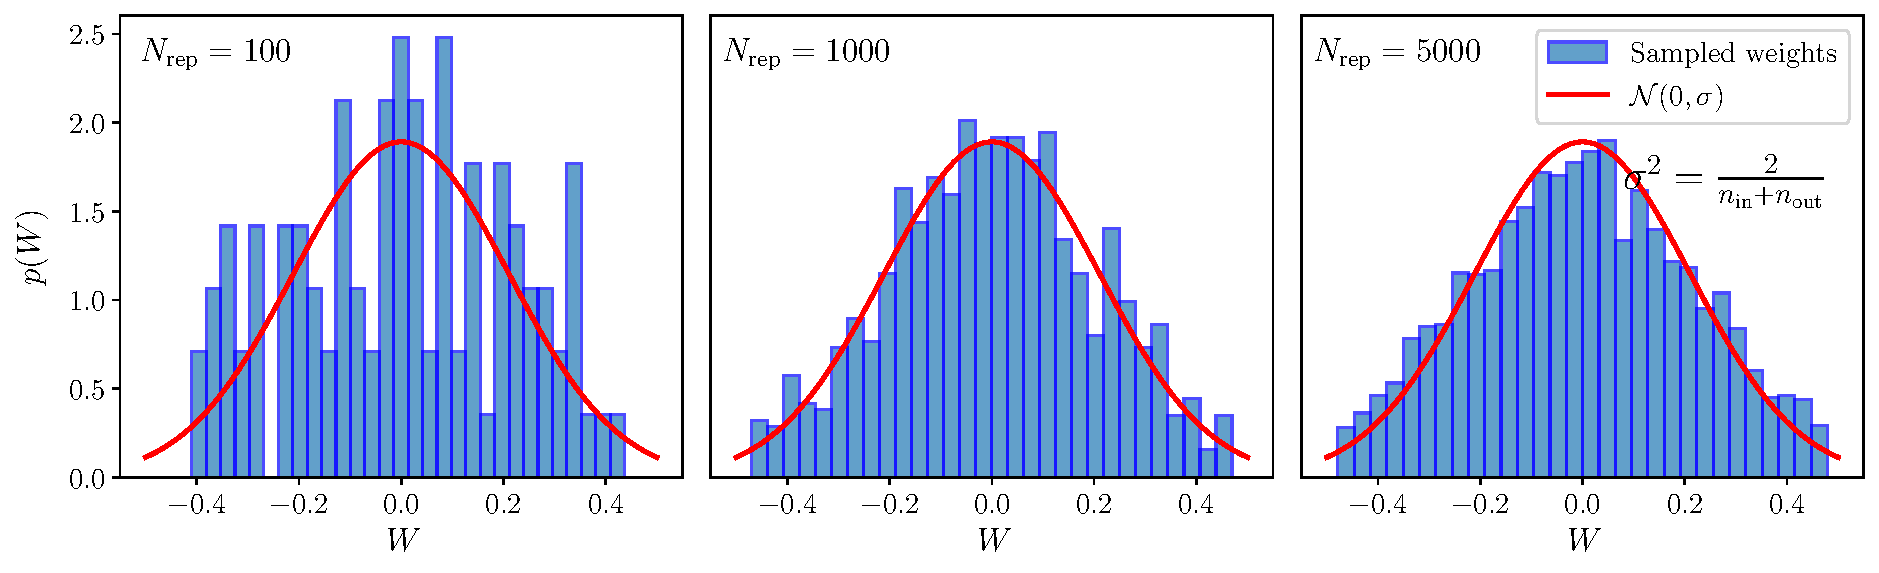
\includegraphics[width=0.95\textwidth]{section_2/weight_distribution.pdf}
  \caption{Sampled distribution of a selected weight in function of the
  number of replicas. The red line represent the underlying Gaussian distribution
  from which the weights are drawn. As the number of replicas is increased the 
  distribution of the weight converges to the expected Gaussian.}
  \label{fig:weight_distribution}
\end{figure}
% ===================================
The Glorot normal initialiser draws each weight and bias of the NN from independent Gaussian
distributions, denoted $p_w$ and $p_b$ respectively, centred at zero and with variances
rescaled by the number of nodes in adjacent layers,
\begin{equation}
    \label{eq:RescaledGlorotVariances}
    \frac{C^{(\ell)}_{w}}{\sqrt{n_{\ell-1} + n_{\ell}}}\, ,
    \quad \frac{C^{(\ell)}_{b}}{\sqrt{n_{\ell-1} + n_{\ell}}}\, .
\end{equation}
Following the NNPDF prescription, we have $C^{(\ell)}_{w}=C^{(\ell)}_{b}=1$.
Fig.~\ref{fig:weight_distribution} shows the binned distribution of a selected
weight in the network as a function of the number of replicas. Together with the
histogram, the underlying Gaussian, as dictated by the Glorot normal
initialisation, is also shown. The figure illustrates that the distribution of
the weights converges to the expected Gaussian as the number of replicas increases.

The probability distribution of the NN parameters induces a probability distribution for the
preactivations,
\begin{align}
    \label{eq:PreactAtInit}
    p\left(\phi^{(\ell)}\right)
      &= \int \mathcal{D}w\, p_w(w)\,
        \mathcal{D}b\, p_b(b)\, \prod_{i,\alpha}
        \delta\left(
          \phi^{(\ell)}_{i\alpha} - \sum_{j} w^{(\ell)}_{ij}
          \rho\left(\phi^{(\ell-1)}_{j\alpha}\right)
          - b^{(\ell)}_i
          \right)\, .
\end{align}
Note that, here and in what follows, $p(\phi^{(\ell)})$ denotes the joint probability for all the
$n_{\ell}\times\ngrid$ components of $\phi^{(\ell)}$,
\begin{align}
    \label{eq:ExplIndices}
    p\left(\phi^{(\ell)}\right) = p\left(\phi^{(\ell)}_{1,\alpha_1}, \phi^{(\ell)}_{2,\alpha_1}, \ldots,
        \phi^{(\ell)}_{n_\ell,\alpha_1}, \phi^{(\ell)}_{1,\alpha_2}, \ldots, \phi^{(\ell)}_{n_\ell,\alpha_2},
        \ldots,
        \phi^{(\ell)}_{n_\ell,\ngrid}\right)\, .
\end{align}
This duality between parameter-space and function-space provides a powerful framework to study
the behaviour of an ensemble of NNs, and in particular the symmetry properties of the distribution
$p(\phi^{(\ell)})$, see \eg~\cite{Maiti:2021fpy}. Working in parameter space, \ie\ computing the
expectation values of correlators of fields as integrals over the NN parameter, one can readily
show that
\begin{align}
    \label{eq:NeurRotInv}
    \mathbb{E}\left[
        R_{i_1j_1} \phi^{(n_\ell)}_{j_1 \alpha_1} \ldots
        R_{i_nj_n} \phi^{(n_\ell)}_{j_n \alpha_n}
    \right] =
    \mathbb{E}\left[
        \phi^{(n_\ell)}_{i_1 \alpha_1} \ldots
        \phi^{(n_\ell)}_{i_n \alpha_n}
    \right]\, ,
\end{align}
where $R$ is an orthogonal matrix in $\text{SO}(n_{\ell})$. Eq.\eqref{eq:NeurRotInv} implies
that the probability distribution in Eq.~\eqref{eq:PreactAtInit} is also invariant under rotations,
and therefore it can only be a function of $\text{SO}(n_{\ell})$ invariants. Therefore
\begin{align}
    \label{eq:PriorAction}
    p\left(\phi^{(n_\ell)}\right) =
        \frac{1}{Z^{(\ell)}} \exp\left(-S\left[\phi^{(\ell)}_{\alpha_1}
            \cdot \phi^{(\ell)}_{\alpha_2}\right]\right)\, ,
\end{align}
where
\begin{align}
    \label{eq:PhiInvariant}
    \phi^{(\ell)}_{\alpha_1}
            \cdot \phi^{(\ell)}_{\alpha_2} =
    \sum_{i=1}^{n_\ell} \phi^{(\ell)}_{i \alpha_1} \phi^{(\ell)}_{i \alpha_2}\, .
\end{align}
The action can be expanded in powers of the invariant bilinear,
\begin{align}
    \label{eq:ExpandAction}
    S\left[\phi^{(\ell)}_{\alpha_1}
            \cdot \phi^{(\ell)}_{\alpha_2}\right] =
        \frac12 \gamma^{(\ell)}_{\alpha_1\alpha_2}
            \phi^{(\ell)}_{\alpha_1} \cdot \phi^{(\ell)}_{\alpha_2} +
            \frac{1}{8 n_{\ell-1}} \gamma^{(\ell)}_{\alpha_1\alpha_2,\alpha_3\alpha_4}
            \phi^{(\ell)}_{\alpha_1} \cdot \phi^{(\ell)}_{\alpha_2} \,
            \phi^{(\ell)}_{\alpha_3} \cdot \phi^{(\ell)}_{\alpha_4} + O(1/n_{\ell-1}^2)\, ,
\end{align}
so that the probability distribution is fully determined by the couplings 
$\gamma^{(\ell)}$.\footnote{
    We have denoted {\em all}\ couplings by $\gamma^{{(\ell)}}$. Different couplings 
    are indentified by the number of indices, so that $\gamma^{(\ell)}_{\alpha_1\alpha_2}$ 
    is a two-point coupling, $\gamma^{(\ell)}_{\alpha_1\alpha_2,\alpha_3\alpha_4}$ is a four-point 
    coupling, etc. 
} 
In
Eq.~\eqref{eq:ExpandAction}, we have factored out inverse powers of $n_\ell$ for each coupling.
With this convention, and with the scaling of the parameters variances in
Eq.~\eqref{eq:RescaledGlorotVariances}, the couplings in the action are all $O(1)$
in the limit where $n_\ell\to\infty$.
As a consequence, the probability distribution at initialisation is a multidimensional Gaussian at
leading order -- \ie\ $\mathcal{O}(1)$ -- in $1/n_\ell$, with quartic corrections that are $O(1/n_\ell)$, while higher powers
of the invariant bilinear are suppressed by higher powers of the width of the layer. This power counting
defines an effective field theory, where deviations from Gaussianity can be computed in perturbation
theory to any given order in $1/n_\ell$, see \eg\ Ref.~\cite{Roberts:2021fes} for a detailed
presentation of these ideas. While the actual calculations become rapidly cumbersome, the
conceptual framework is straightforward.

At leading order, the second and fourth cumulant are respectively
\begin{align}
    &\langle \phi^{(\ell)}_{i_1,\alpha_1} \phi^{(\ell)}_{i_2,\alpha_2}\rangle
      = \delta_{i_1 i_2} K^{(\ell)}_{\alpha_1\alpha_2} + O(1/n_{\ell-1})\, , \\
    &\langle \phi^{(\ell)}_{i_1,\alpha_1} \phi^{(\ell)}_{i_2,\alpha_2}
      \phi^{(\ell)}_{i_3,\alpha_3} \phi^{(\ell)}_{i_4,\alpha_4}\rangle_c
      = O(1/n_{\ell-1})\, ,
\end{align}
where
\begin{equation}
    \label{eq:DefineKmat}
    K^{(\ell)}_{\alpha_1\alpha_2} = \left(\gamma^{(\ell)}\right)^{-1}_{\alpha_1\alpha_2}\, .
\end{equation}
The ``evolution'' of the couplings as we go deep in the NN, \ie\ the dependence of the couplings on
$\ell$, is governed by Renormalization Group (RG) equations, which preserve the power counting in
powers of $1/n_{\ell}$. At leading order,
\begin{align}
    K^{(\ell+1)}_{\alpha_1\alpha_2} &=
      \left.
      C_b^{(\ell+1)} + C_w^{(\ell+1)} \frac{1}{n_\ell}
      \langle \vec{\rho}^{\,(\ell)}_{\alpha_1} \cdot
      \vec{\rho}^{\,(\ell)}_{\alpha_2} \rangle
      \right|_{O(1)} \\
      \label{eq:RecursionForK}
      &= C_b^{(\ell+1)} + C_w^{(\ell+1)} \frac{1}{n_\ell}
      \langle \vec{\rho}^{\,(\ell)}_{\alpha_1} \cdot
      \vec{\rho}^{\,(\ell)}_{\alpha_2} \rangle_{K^{(\ell)}}\, ,
\end{align}
where
\begin{align*}
    \frac{1}{n_\ell}
      \langle \vec{\rho}^{\,(\ell)}_{\alpha_1} \cdot
      \vec{\rho}^{\,(\ell)}_{\alpha_2} \rangle_{K^{(\ell)}} =
    \int \prod_{\alpha}d\phi_\alpha\,
      \frac{e^{-\frac12 \left(K^{(\ell)}\right)^{-1}_{\beta_1\beta_2}
        \phi_{\beta_1} \phi_{\beta_2}}}
        {\left|2\pi K^{(\ell)}\right|^{1/2}}\,
        \rho(\phi_{\alpha_1}) \rho(\phi_{\alpha_2})\, .
\end{align*}
Eq.~\eqref{eq:RecursionForK} can be iterated using the NNPDF architecture,
yielding the covariance at initialisation for various depths. These are compared
with the empirical covariance computed from an ensemble of 100 replicas in
Fig.~\ref{Fig:KRecursionOne} for the first deep-layer and in
Fig.~\ref{Fig:KRecursionTwo} for the second-deep layer and output layer. The
agreement between the theoretical prediction and the empirical computation is
excellent, confirming the validity of the large-network expansion even for
networks of moderate size, as those used in the NNPDF fits.

\begin{figure}[t]
    \centering
    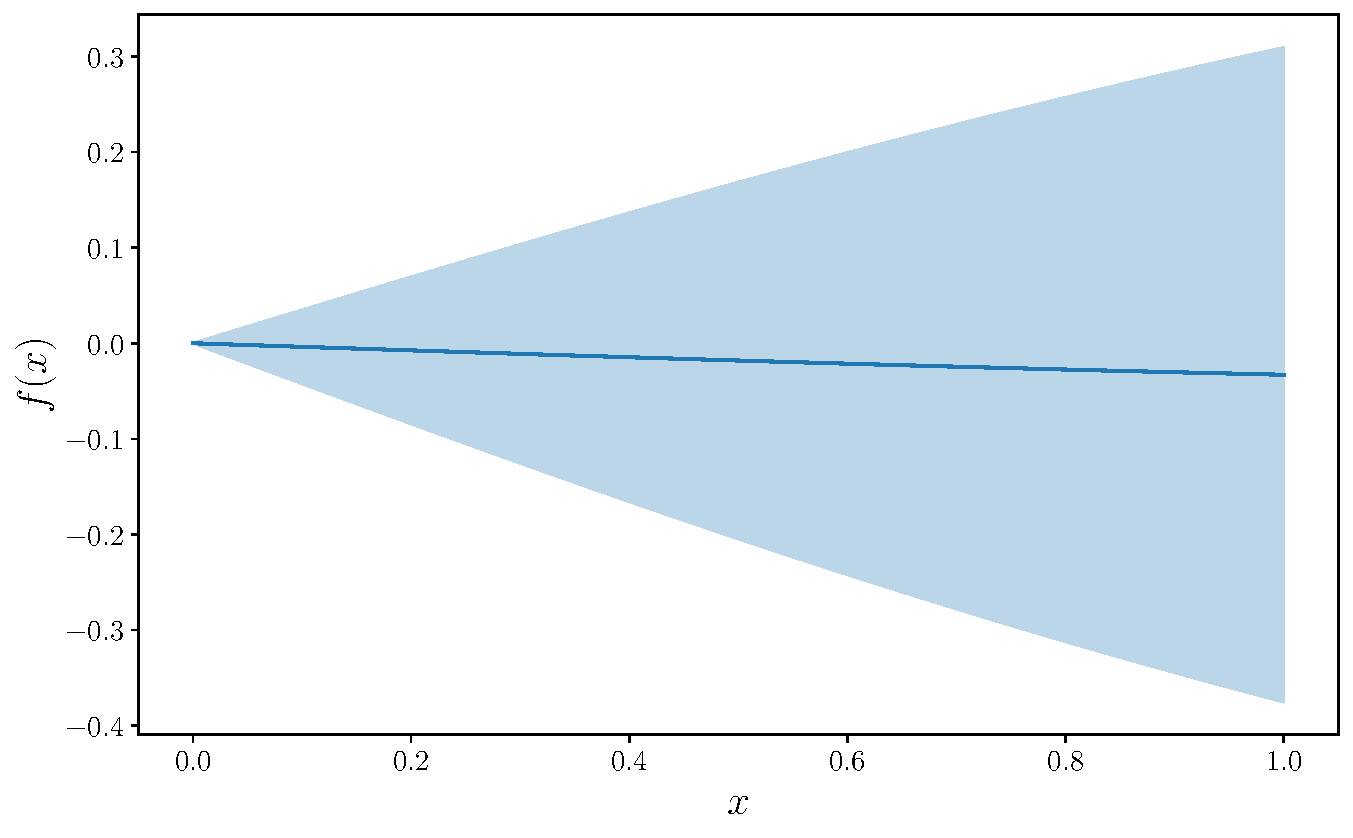
\includegraphics[width=0.45\textwidth]{section_2/prior.pdf}
    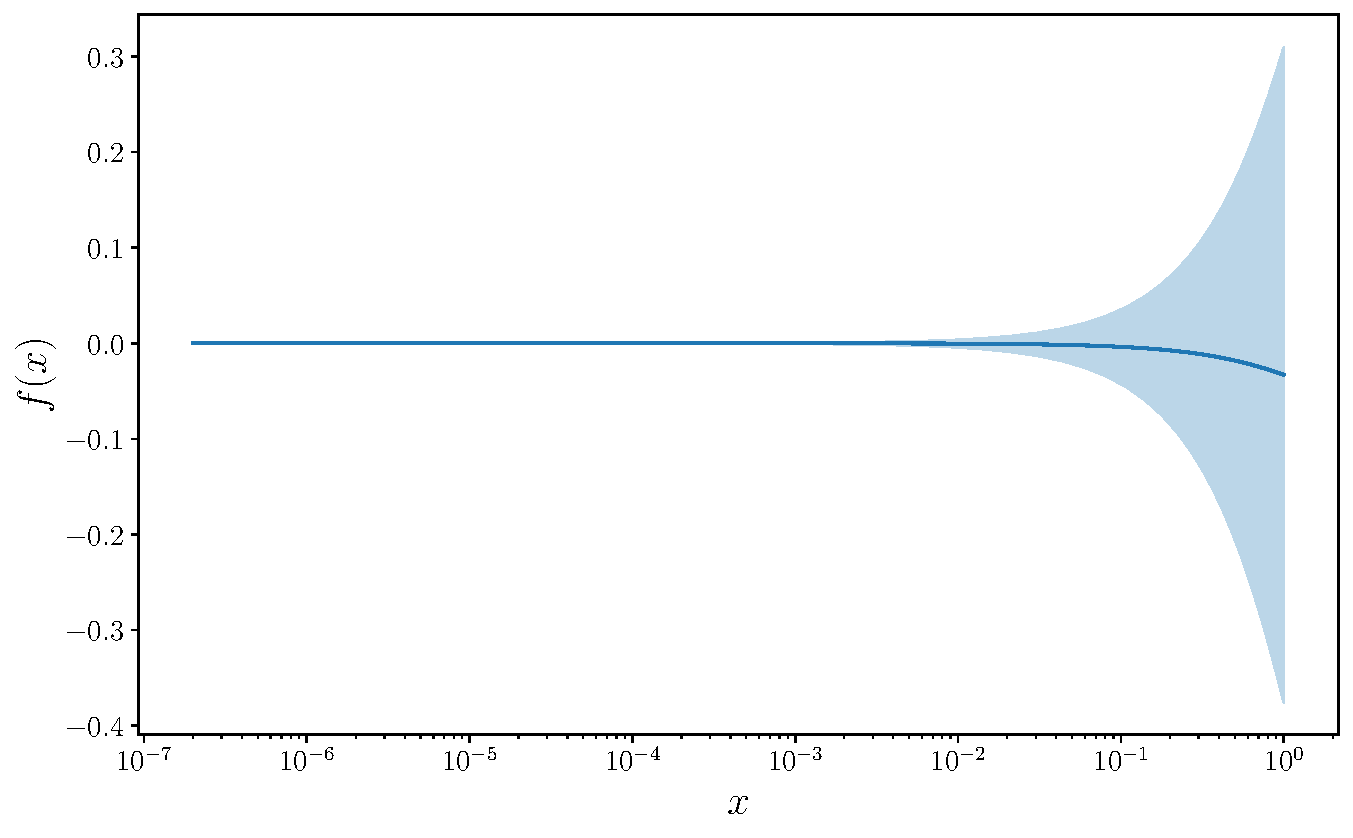
\includegraphics[width=0.45\textwidth]{section_2/prior_log.pdf}
    \caption{Ensemble of neural networks at initialisation in linear (left) and logarithm (right) scale.
    The blue line represents the mean value computed over an ensemble of 100 replicas, while the
    shaded band represents the one-sigma uncertainty computed as the variance over the same ensemble.
    In the figure, we show $xT_3$ as used in the following sections.}        
    \label{fig:prior} 
\end{figure}
\begin{figure}[t]
    \centering
    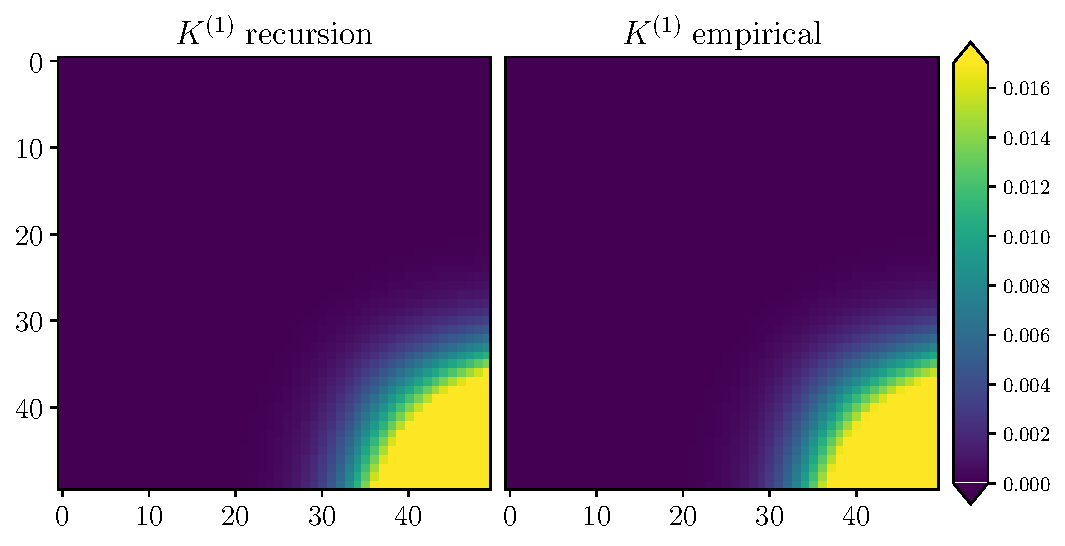
\includegraphics[scale=0.8]{section_2/K1_correlations.pdf}
    \caption{The empirical (left) and analytical (right) covariance matrices $K^{(1)}$ of the first layer
    of the NNPDF architecture. The covariance in the left panel is computed ``bootstrapping'' over an
    ensemble of 100 replicas, initialised using the Glorot normal distribution. The covariance in the right
    panel is obtained by solving Eq.~\eqref{eq:RecursionForK} numerically.
    \ldd{What is the level of the agreement?}
    \label{Fig:KRecursionOne}
    }
\end{figure}

\begin{figure}[t]
    \centering
    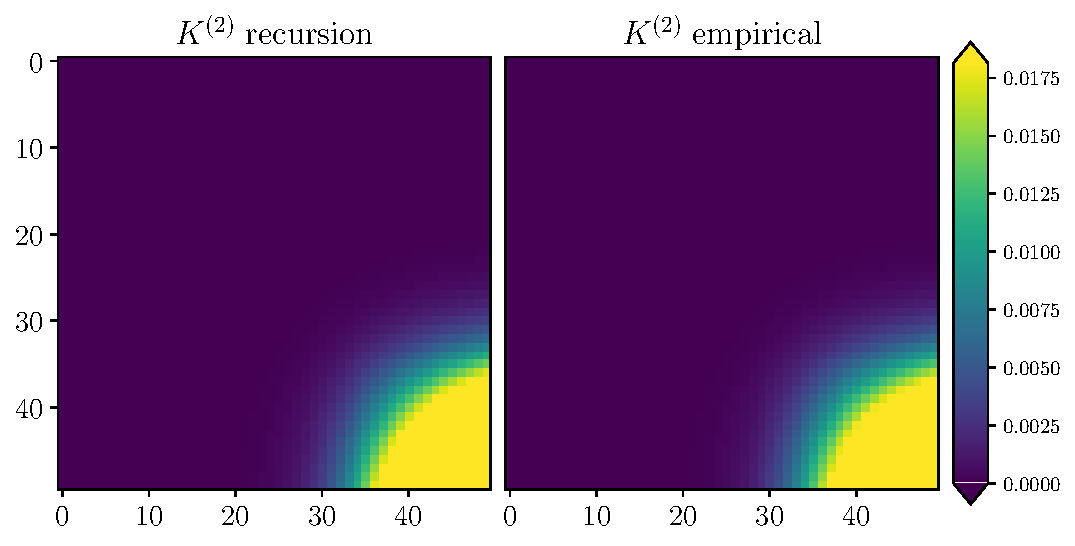
\includegraphics[scale=0.45]{section_2/K2_correlations.pdf}
    \hspace{0.5cm}
    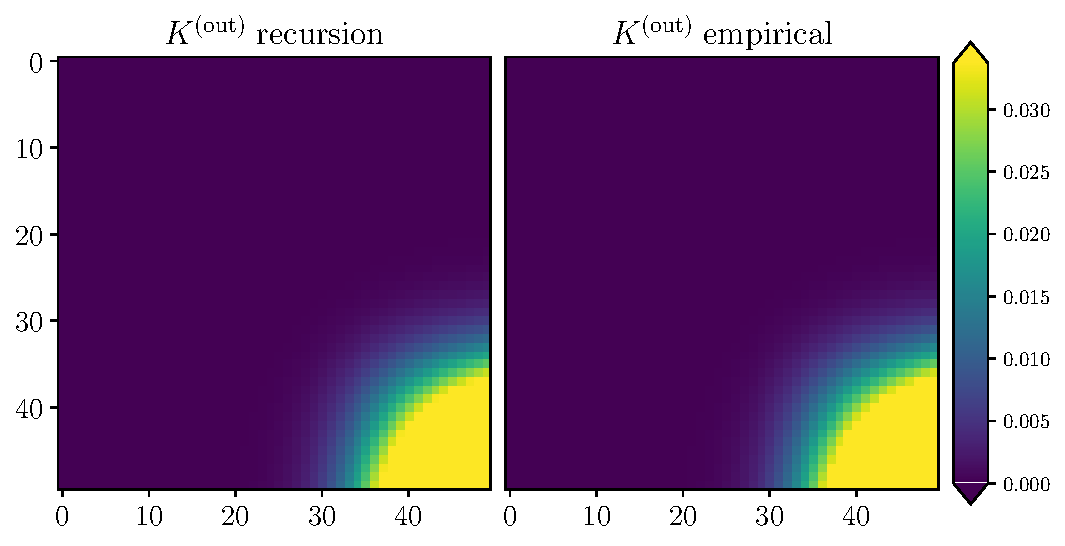
\includegraphics[scale=0.45]{section_2/K3_correlations.pdf}
    \caption{Same as Fig.~\ref{Fig:KRecursionOne}, but for the second (top) and
    third (bottom) layers of the NNPDF architecture.}
    \ldd{What is the level of the agreement?}
    \label{Fig:KRecursionTwo}
\end{figure}
\begin{figure}[t]
    \centering
    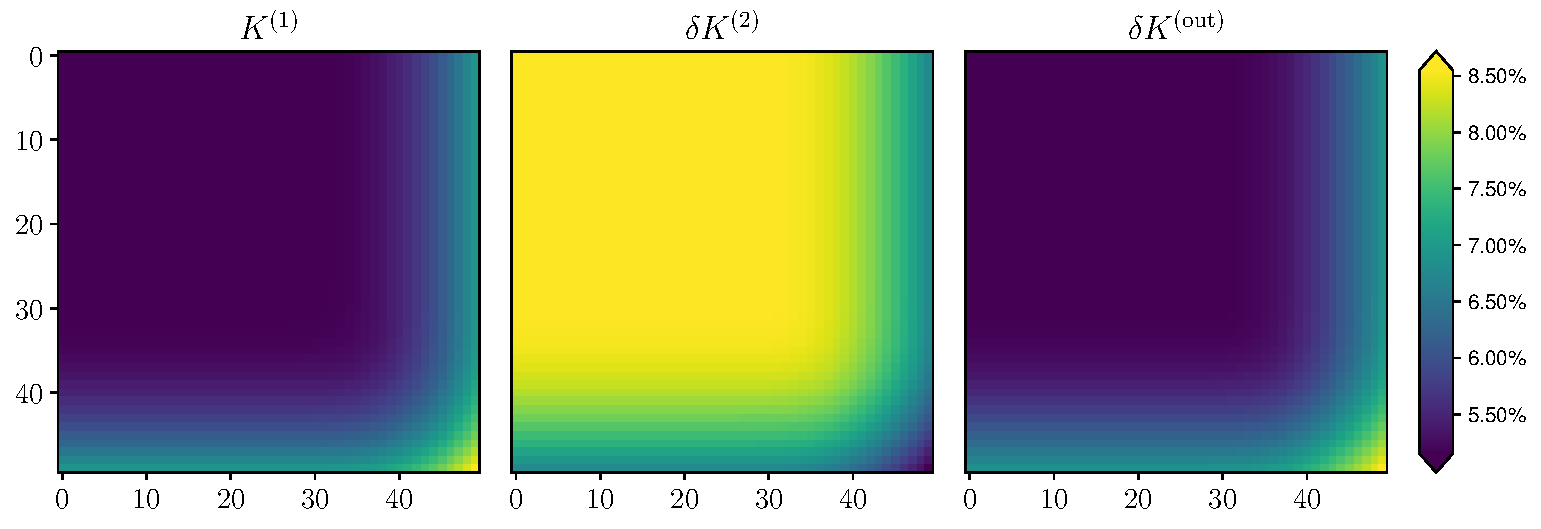
\includegraphics[width=0.9\textwidth]{section_2/delta_K.pdf}
    \caption{Here we show the relative difference between the empirical
    kernel computed from an ensemble of 100 replicas at initialisation
    and the theoretical prediction obtained by iterating
    Eq.~\eqref{eq:RecursionForK} for the three layers of the NNPDF architecture.
    \ac{Does this give more information than the previous plots?}}
\end{figure}


As a consequence of the symmetry of the probability distribution, the mean value
of the fields at initialisation needs to vanish, while their variance at each
point $x_\alpha$ is given by the diagonal matrix elements of $K^{(\ell)}$. In
the following, we will consider neural networks with the NNPDF architecture, but
will consider only one output layer. The mean and variance of the output at
initialisation are shown in Fig.~\ref{fig:prior} for an ensemble of
$\nreps=100$. The central value is computed as discussed above in
Eq.~\eqref{eq:ReplicaEnsemble},
\begin{align}
    \label{eq:MeanValAtInit}
    \bar{f}_{i\alpha} = \bar{f}_{i}(x_\alpha) = \frac{1}{\nreps} \sum_{k=1}^{\nreps} f^{(k)}_i(x_\alpha)\, ,
\end{align}
and the variance $\sigma^2_{i\alpha}$ is computed using the same formula with
\begin{align}
    \label{eq:VarAtInit}
    O(f) = \frac{\nreps}{\nreps-1} \left(f_i(x_\alpha) - \bar{f}_{i}(x_\alpha)\right)^2\, .
\end{align}

\FloatBarrier

\section{Training Dynamics and the Neural Tangent Kernel}
\label{sec:Training}

Having defined the physical context of this work and established some properties
of the neural network at initialisation, we now turn to the optimisation
process. In the context of machine learning, specifically when dealing with
neural networks, optimisation is an iterative algorithm that updates the
parameters of the network in order to minimise a figure of merit defined
appropriately. Due to the large number of parameters that characterise a neural
network, the figure of merit (also known as \textit{error function},
\textit{loss function}, or simply \textit{loss}) is a non-convex
high-dimensional function, posing a challenge in the minimisation task. In
addition, in order to avoid \textit{over-} and \textit{under-learning}, these
training algorithms are paired with the so-called \textit{stopping criterion},
which specifies the optimal condition to end the training process.

In practice, this task is tackled by using gradient methods where the direction
towards the minimum is defined by the gradient of the loss function. These
methods are usually improved by including, for instance, stochasticity and
information on previous iterations. A detailed overview of these extended
gradient methods is beyond the scope of this work. In the context of PDF
determinations, the NNPDF collaboration makes intensive use of these tools and
the reader is encouraged to refer to Ref.~\cite{NNPDF:2021njg} for an extensive
discussion.

Our main aim in this paper is understanding the dynamics driving the training
process. Indeed, while these algorithms have achieved remarkable empirical
success, a theoretical understanding of the optimization process remains
elusive. Therefore, we work in a simplified setting where we consider the
simplest gradient method, \textit{i.e.} Gradient Descent (GD), and and data that
depend linearly on the unknwon PDFs, as shown in Eq.~\eqref{eq:TheoryPred}.
Furthermore, we do not split the dataset between training and
validation\footnote{We are aware that such a framework has limited applicability
in the context of PDF determination, and we are far from assuming this as an
optimal choice. Again, the focus remain on the methodological aspects rather
than the underlying physics.} The generalization to other minimizers and
non-linear data is left to future investigations, but is expected to yield
qualitatively similar results. Finally, we remark that the results in this
section, although obtained having in mind neural networks, apply to any generic
parametrization of the unknown function, whether it is a polynomial or a
kernel~\cite{Costantini:2025wxp}.

\subsection{Training in Functional Space}
\label{sec:GradFlow}

Gradient descent is described as a continuous flow of the parameters $\theta$ in
training time $t$ along the negative gradient of the loss function
$\mathcal{L}$. Following from the parameter-space/function-space duality
introduced in Sec.~\ref{sec:Init}, we aim at rephrasing the optimisation process
of GD in the space of the network output $f$. To ease the mathematical
tractability, we employ the continuous version of GD, which has been
shown~\cite{barrett2022igr} to match the discretised version as long as the
learning rate is small enough. The continuous Gradient Flow (GF) is then given
by
\begin{align}
    \label{eq:GradientFlowDef}
    \ddt &\theta_{t,\mu} = -\nabla_\mu \mathcal{L}_t\, ,
\end{align}
where $\theta_{t,\mu}$ and $\mathcal{L}_t$ identify respectively the parameter
and the loss function at training time $t$. We focus here on quadratic loss
functions that are obtained as the negative logarithm of Gaussian data
distributions around their theoretical predictions,
\begin{align}
    \label{eq:QuadLoss}
    \mathcal{L}_t = \frac12 \left(Y - T[f_t]\right)^T C_Y^{-1} \left(Y - T[f_t]\right)\, ,
\end{align}
where $f_t$ is the output of the network at training time $t$, which follows
from the time-dependence of the internal parameters. Here $C_Y$ is the
covariance of the data, which includes statistical and systematic errors given
by the experiments and also any theoretical error, like \eg\ missing higher
orders in the theoretical predictions. Indices that are summed over are
suppressed to improve the clarity of the equations. Note that the loss function
at training time $t$ is computed using the theoretical prediction $T[f_t]$, \ie\
the result of Eq.~\eqref{eq:TheoryPred} computed using the fields at training
time $t$. For a quadratic loss, the gradient is
\begin{align}
    \nabla_\mu \mathcal{L}_t = - \left(\nabla_\mu f_t\right)^T \left(\frac{\partial T}{\partial f}\right)_t
      C_Y^{-1} \epsilon_t\, ,
\end{align}
where, writing explicitly the data index,
\begin{align}
    \label{eq:EpsDef}
    \epsilon_{t,I} = Y_I - T_I[f_t]\, , \quad I=1, \ldots, \ndat\, .
\end{align}
For the specific case of a quadratic loss function, the gradient is proportional
to $\epsilon_t$, which is the difference between the theoretical prediction and
the data at training time $t$. If at some point during the training the
theoretical predictions reproduce all the data, the training process ends. A
further simplification is obtained in the case of data that depend linearly on
the unknown function $f$. In the specific case of NNPDF fits, the integrals in
Eq.~\eqref{eq:TheoryPred} are approximated by a Riemann sum over the grid of $x$
points,
\begin{align}
    \label{eq:FKTabDef}
    T_I[f] \approx \sum_{i=1}^{\nflav}\sum_{\alpha=1}^{\ngrid} \FKtab_{Ii\alpha} f_{i\alpha}\, ,
\end{align}
and hence
\begin{align}
    \label{eq:dTbydf}
    \left(\frac{\partial T_I}{\partial f_{i\alpha}}\right)_t =
        \FKtab_{Ii\alpha}\, ,
\end{align}
which is independent of $t$. With simple algebraic steps, the flow of parameters
$\theta$ can be translated into a flow for the fields,
\begin{align}
    \label{eq:NTKFlow}
    \ddt &f_{t,i_1\alpha_1} = (\nabla_\mu f_{t,i_1\alpha_1}) \ddt \theta_\mu =
      \Theta_{t,i_1\alpha_1i_2\alpha_2}
      \FKtabT_{i_2\alpha_2I} \left(C_Y^{-1}\right)_{IJ} \epsilon_{t,J}\, ,
\end{align}
where we have defined the Neural Tangent Kernel~\cite{jacot2018neural}
\begin{align}
    \label{eq:NTKDef}
    \Theta_{t,i_1\alpha_1i_2\alpha_2} = \sum_\mu
    \nabla_\mu f_{t,i_1\alpha_1} \nabla_\mu f_{t,i_2\alpha_2}\, .
\end{align}
As it will become more clear in later, the NTK provides a powerful framework for
understanding neural network dynamics during training. Originally developed by
Jacot et al.~\cite{jacot2018neural} to analyse infinite-width feed-forward
networks, the NTK theory has since been extended to diverse architectures
including convolutional networks~\cite{arora2019exact} and recurrent
networks~\cite{alemohammad2021recurrent}. This theoretical framework has proven
invaluable for characterizing learning dynamics and generalization properties
across various network designs. 

In order to facilitate the discussion in Sec.~\ref{sec:Lazy},
Eq.~\eqref{eq:NTKFlow} can be rewritten in a more compact form. We first omit
the indices such that, for instance,
\begin{align}
  \left(\frac{\partial T}{\partial f}\right)_t = \FKtab\, , \quad
  \Theta_t = \left(\nabla_\mu f_t\right) \left(\nabla_\mu f_t\right)^T\, .
  \label{eq:dTdfForLinearObs}
\end{align}
Then, using the definition of the error in Eq.~\eqref{eq:EpsDef}, we can rewrite
Eq.~\eqref{eq:NTKFlow} as follows
\begin{align}
    \label{eq:FlowEquationNoIndices}
    \ddt f_t = -\Theta M f_t + b\, ,
\end{align}
where
\begin{align}
    M &= \FKtabT C_Y^{-1} \FKtab\, , \quad b = \Theta \FKtabT C_Y^{-1} Y\, .
\end{align}
Here $M$ is a positive-semidefinite matrix that depends only on the data and the
theoretical predictions, while $b$ is a vector that depends also on the data.

Before moving to the next subsection, a few comments are due. First, although
derived in the context of neural networks, these equations do not refer to a
specific parameterization. Indeed, these remain valid even when an explicit
functional form to parametrize the PDFs is chosen, as \eg in
Refs.~\cite{Bailey:2020ooq,Hou:2019efy,Costantini:2025wxp}. Second, it is
interesting to observe that the flow equation,
Eq.~\eqref{eq:FlowEquationNoIndices}, depends on two matrices, $\Theta$ and $M$.
The former encodes the model dependence, while the latter brings physical
information. The interplay between these two matrices is crucial for
understanding the training dynamics, as it will be discussed in
Sec.~\ref{sec:NTKAlign}. Finally, the NTK derived in Eq.~\ref{eq:NTKDef} is
inherently time-dependent in a complex way, which precludes any attempt in
integrating Eq.~\ref{eq:FlowEquationNoIndices} analytically. We will come back
to this point in Sec.~\ref{sec:Lazy}, and we now turn to discussing the
properties of the NTK during training.

\subsection{Inside the Training Dynamics: an NTK perspective}

From Eqs.~\eqref{eq:NTKDef} and~\eqref{eq:FlowEquationNoIndices}, we observe
that the NTK encodes the dependence on the architecture of the network and
governs its training dynamics. The analysis of the NTK properties is thus
crucial for understanding the behaviour of the network during training. We first
discuss the properties of the NTK at initialisation, before moving to the
training phase, where we provide a detailed study of the NTK in the context of
the NNPDF methodology.

% ===================================
\begin{figure}[t!]
  \centering
  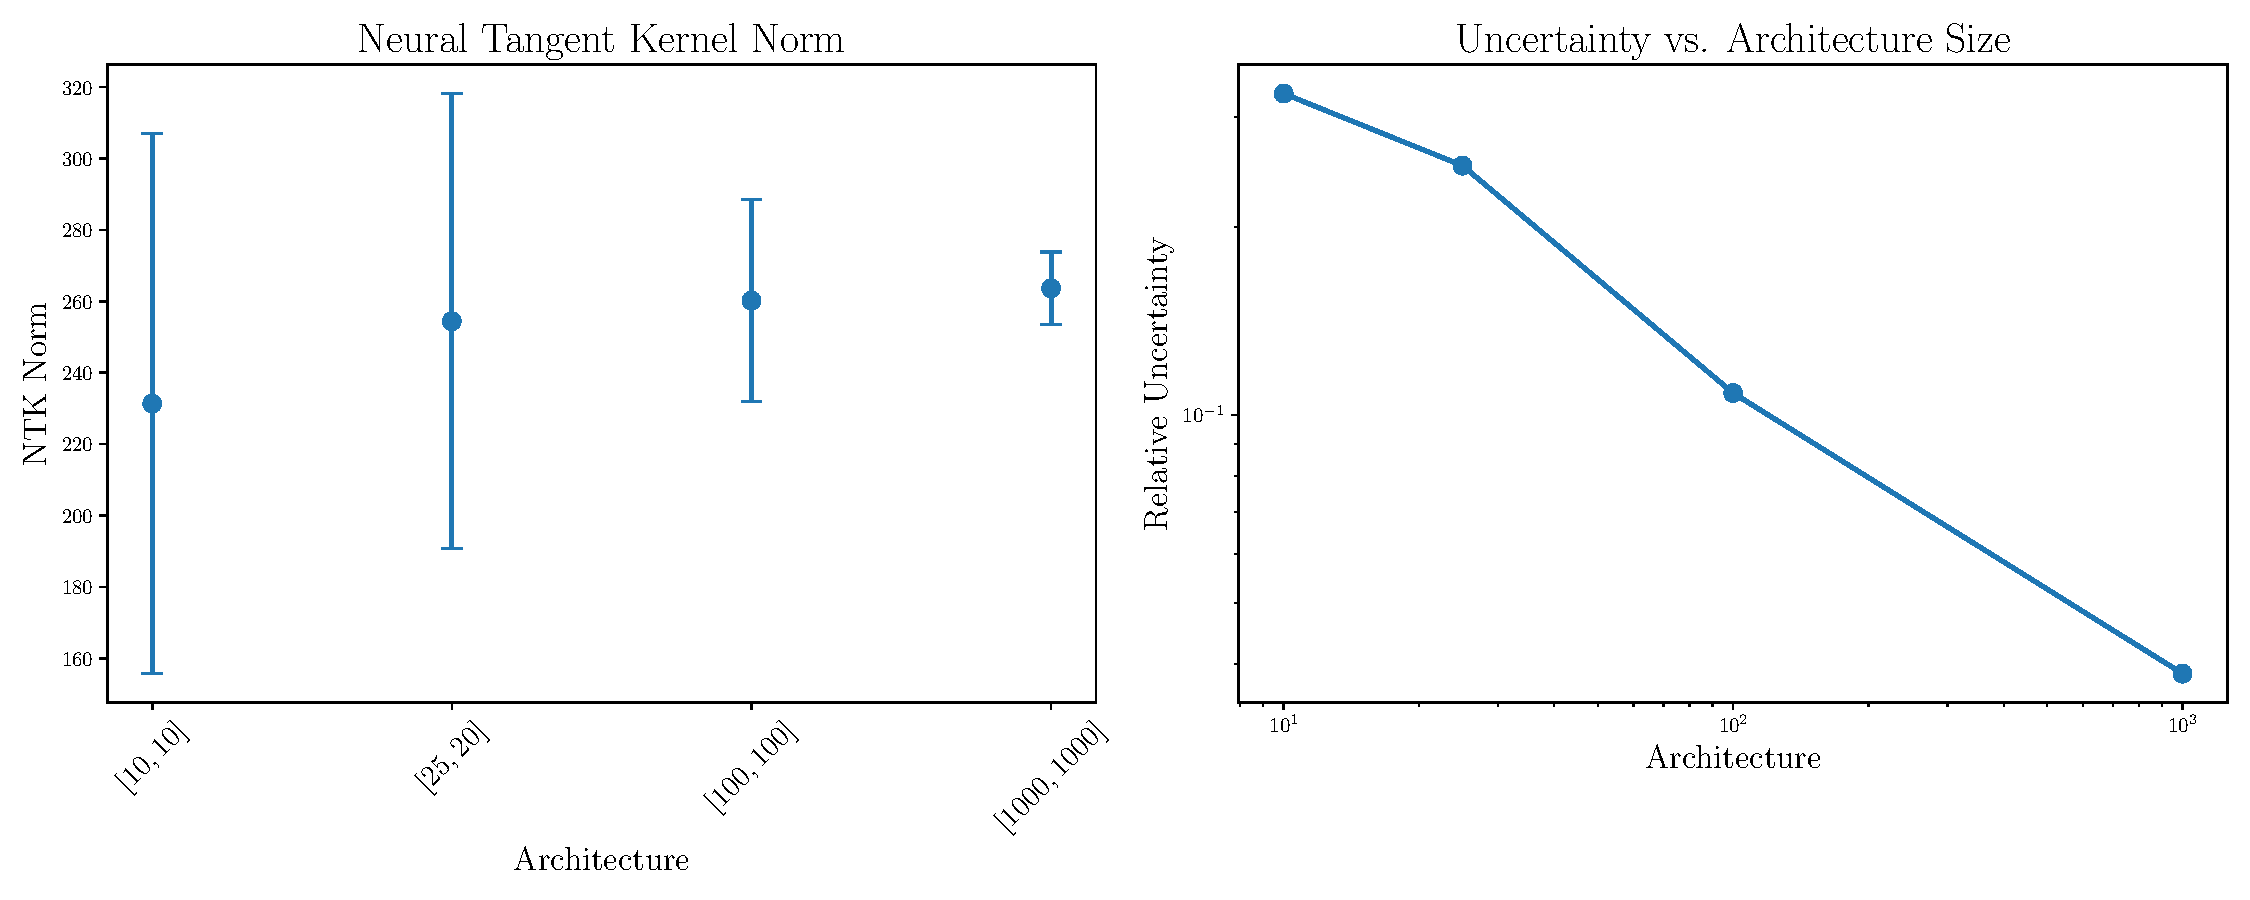
\includegraphics[width=0.90\textwidth]{figs/section_3/ntk_initialization_with_uncertainty.pdf}
  \caption{Frobenius norm of the NTK at initialisation, $\lVert \Theta_0
  \rVert$, in function of the width of the network. On the left, the central
  values and uncertainty bands are obtained as the mean and one-sigma deviation
  of the ensemble of networks. The plot on the right shows the relative
  uncertainty.}
  \label{fig:NTKInit}
\end{figure}
% ===================================

\subsubsection{NTK at Initialization}
\label{sec:NTKAtInit}

Before training, the NTK is blind to data and depends, in addition to the
architecture, on the $x$-grid of input and on the architecture, as it can be
seen from Eq.~\eqref{eq:NTKDef}. The NTK is a function of the fields $f$, which
are stochastic variables described by their joint probability distribution as
discussed in Sect.~\ref{sec:Init}. Therefore the NTK is also a stochastic
variable, with its own probability distribution, which we represent as usual as
a set of replicas. 

It is argued in the literature that, in the large-width limit, the variance of
the NTK over the set of replicas tends to zero with the width of the hidden
layers (see, \textit{e.g.}, \cite{Roberts:2021fes}). In order to quantify the
variation of the NTK, we start by computing the Frobenius norm of the NTK over
an ensemble of networks for different architectures. For each architecture, we
consider the mean value and standard deviation of the norm as statistical
estimators of the variations of the NTK. The result is displayed in
Fig.~\ref{fig:NTKInit}. Even though the Frobenius norm is a coaarse indicator of
the variations of the NTK, the figure shows clearly that the variance of the
norm becomes smaller with the size of the network, which is consistent with the
theoretical expectation that the NTK should not fluctuate for infinite-width
networks\footnote{Note that, in addition to the scaling $\mathcal{O}(1/n)$
theoretically predicted for large networks, the uncertainty bands include
bootstrap errors due to the finite size of the ensemble. Using an ensemble of
100 replicas, the bootstrap error on the standard deviation is $\sim 10\%$.}.

% ===================================
\begin{figure}[t]
  \centering
  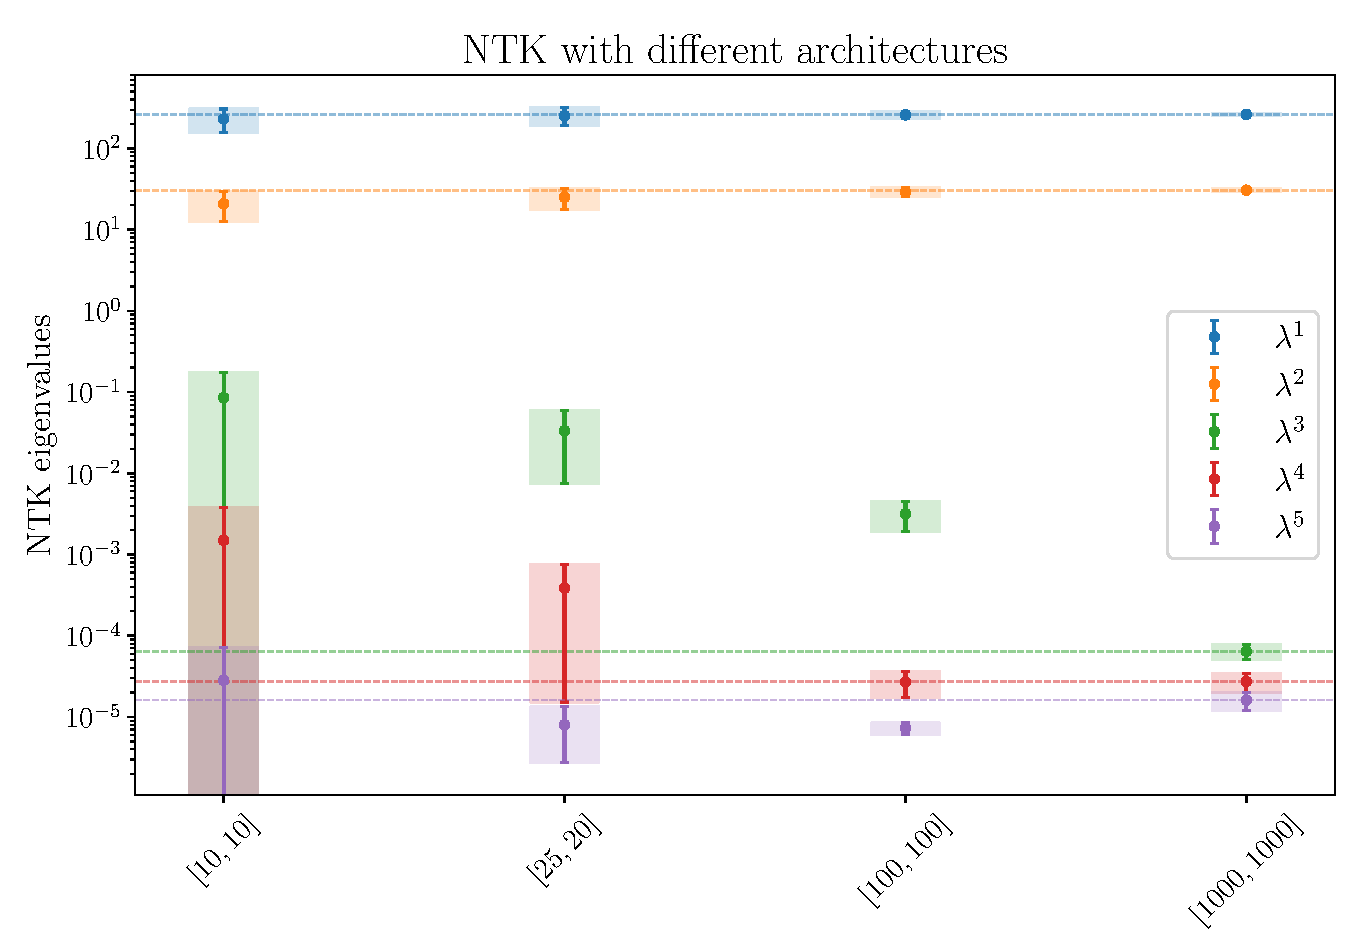
\includegraphics[width=0.45\textwidth]{figs/section_3/ntk_initialization_arch.pdf}
  \caption{Spectrum of the NTK at initialization for the architectures shown in
  Fig.~\ref{fig:NTKInit}. Error bands correspond to one-sigma uncertainties over
  the ensemble of networks.}
  \label{fig:NTKSpectrum}
\end{figure}
% ===================================

In order to get a more quantitative description of the NTK at initialization,
its spectrum is shown in Fig.~\ref{fig:NTKSpectrum} for four different
architectures. Inspecting the plot, we see that the spectrum of the NTK is
heavily hierarchical, and only few eigenvalues are actually
non-zero\footnote{Note that, due to the large difference in magnitude of the
eigenvalues, the finite precision used in our codes introduces noise in the
decomposition, so that small eigenvalues should be effectively considered zero.
We discuss the cut-off tolerance later, when we discuss the training process in
more details.}. This means that only a small subset of active directions can
inform the network during training, as it will be discussed later. Note that, at
least at initialization, these observations do not depend on the architecture.
The eigenvalues in Fig.~\ref{fig:NTKSpectrum} are mostly independent of the size
of the network. There is a downward fluctuation of the third eigenvalue for the
largest architecture that we considered, but we do not have any evidence that
this drop is a physical feature of the system, rather than a fluctuation. the
variance of the set of eigenvalues over replicas decreases with increasing size,
as expected. 

% \FloatBarrier

\subsubsection{NTK During Training}
\label{sec:NTKDuringTraining}

Having established the properties of the NTK at initialisation, we now discuss
its behaviour during training. To do so, we performed a fit of $T_3$ using the
NNPDF methodology with the dataset described in App.~\ref{app:dataset}. We
initialized an ensemble of $\nreps = 100$ replicas with identical architecture,
training each replica independently using GD optimization. As our focus here is
on NTK properties rather than physical predictions, we use generate three sets
of data with controlled noise characteristics -- L0, L1, and L2 -- following the
prescription described in App.~\ref{app:dataset}. Throughout the training
process, we track the evolution of the NTK to understand how the network's
effective dynamics change as it learns the target function.

\paragraph{Onset of Lazy Training} 

% ===================================
\begin{figure}[t]
  \centering
  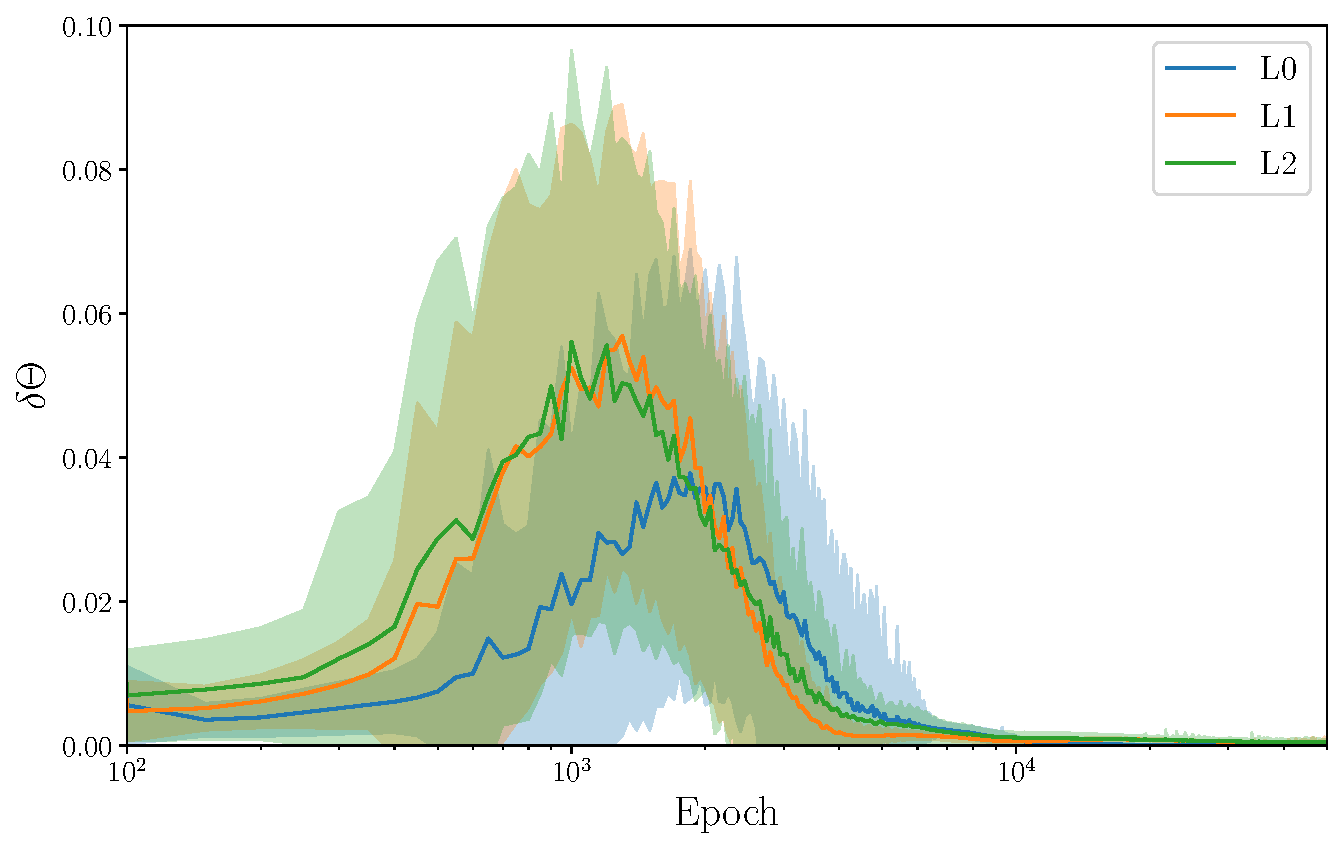
\includegraphics[width=0.45\textwidth]{section_3/delta_ntk.pdf}
  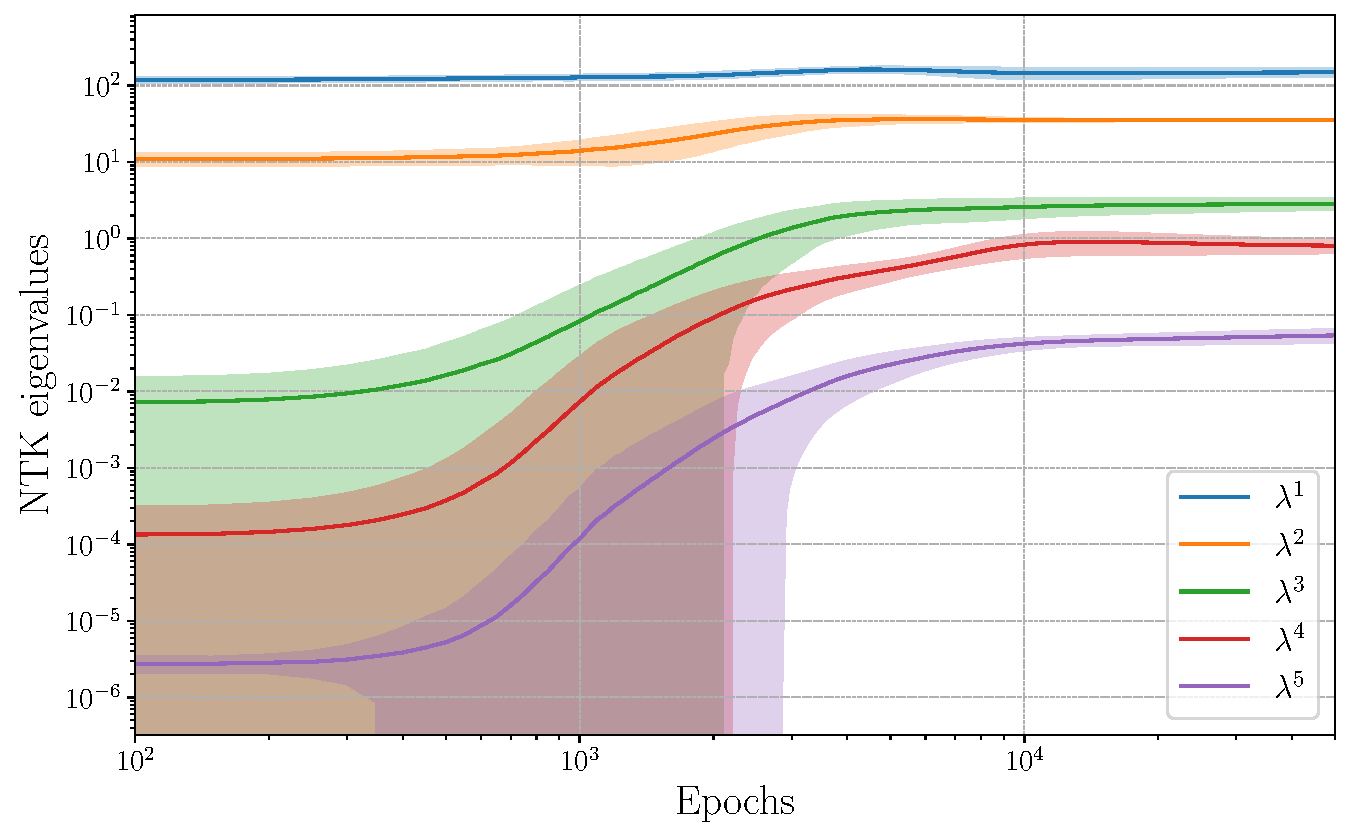
\includegraphics[width=0.45\textwidth]{section_3/ntk_eigvals_single_plot_L0.pdf} 
  \caption{(Left) Relative variation of the NTK during training for L0, L1, and
  L2 data. Error bands correspond to one-sigma uncertainties over the ensemble
  of networks. (Right) Evolution during training of the first five eigenvalues
  of the NTK using L0 data.}
  \label{fig:NTKTime}
\end{figure}
% ===================================

As a first estimator of the variation of the NTK, we show in the left panel of
Fig.~\ref{fig:NTKTime} the Frobenius norm of the variation during training,
normalized by the Frobenius norm of the NTK itself, 
\begin{equation}
\delta \Theta_t = \frac{\lVert \Theta_{t+1} - \Theta_t \rVert}{\lVert \Theta_t \rVert} \;,
\label{eq:DeltaNTK}
\end{equation}
for three different datasets, L0, L1, and L2. Inspecting the plot reveals that
the NTK undergoes significant changes during the initial phase of training, with
the relative variation $\delta \Theta_t$ reaching values as high as $10\%$. This
indicates that our settings differ from the standard picture of lazy training in
the context of very wide networks, as discussed in
Refs.~\cite{jacot2018neural,Roberts:2021fes,lee2019wide}. We also observe that
the variation is more pronounced for L2 data, consistent with the fact that the
architecture needs to accommodate the noise in the data. However, after this
initial phase -- corresponding approximately to the first 20,000 epochs in our
experiment -- the NTK tends to stabilize. These two regions will be referred to
as the \textit{rich} and \textit{lazy} training regimes, respectively, in
keeping with the standard terminology adopted in the literature (see, \eg
Ref.~\cite{fort2020dlvk} where two similar regimes where also identified). We do
not comment any further on the implications of the lazy regime, and postpone the
discussion to Sec.~\ref{sec:Lazy}.

\FloatBarrier

\paragraph{Eigenvalues During Training}

Further insight on the evolution of the NTK can be obtained by studying its
eigensystem as a function of the training time. In the right panel of
Fig.~\ref{fig:NTKTime} we report the variation of the first five eigenvalues of
the NTK, using the standard NNPDF architecture and L0 data. We see that the
hierachical structure observed at initialization is preserved, but the size of
the subdominant eigenvalues increases significantly in the early stages of
training -- by one or two orders of magnitude depending on the specific
eigenvalues. 

% ===================================
\begin{figure}[t]
  \centering
  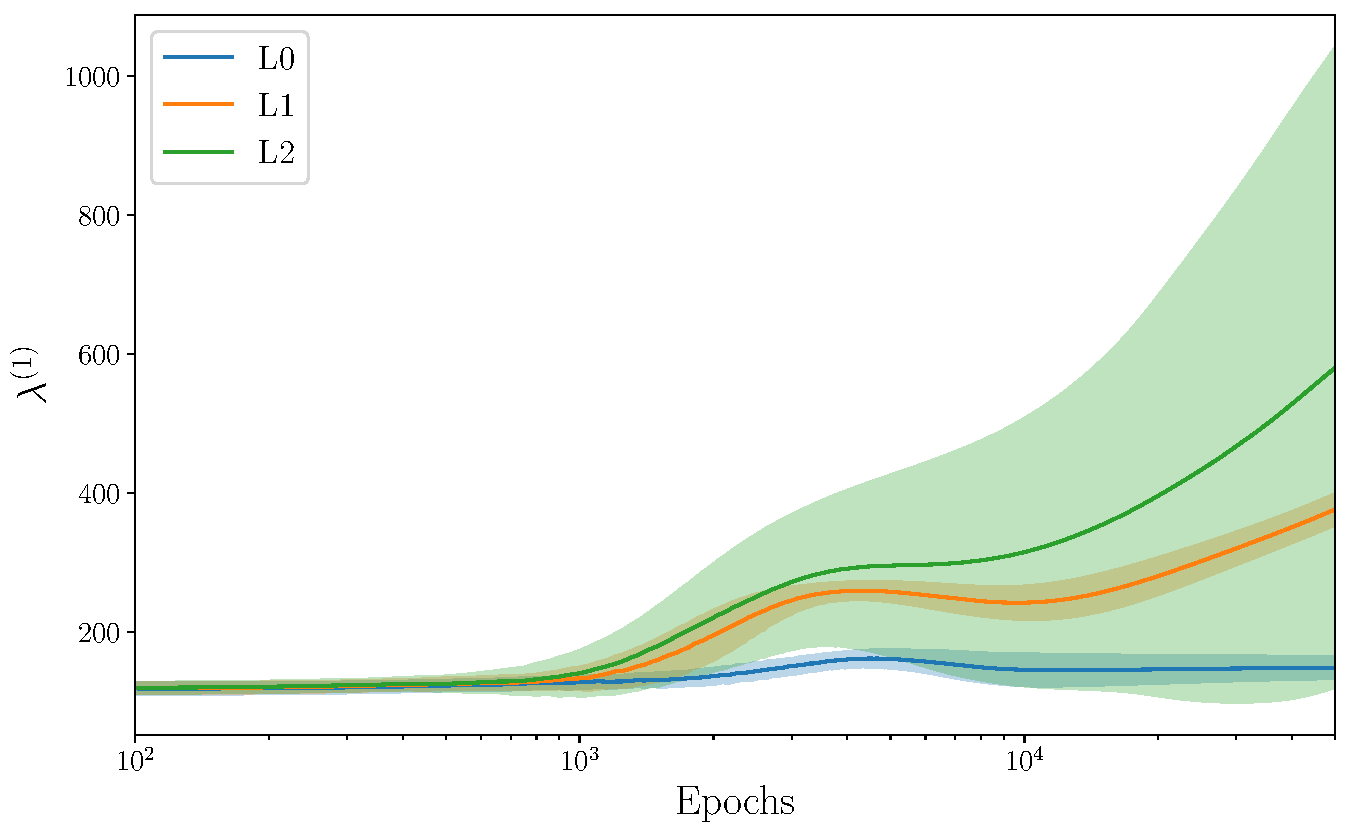
\includegraphics[width=0.30\textwidth]{figs/section_3/ntk_eigvals_L0_L1_L2_n_1.pdf}
  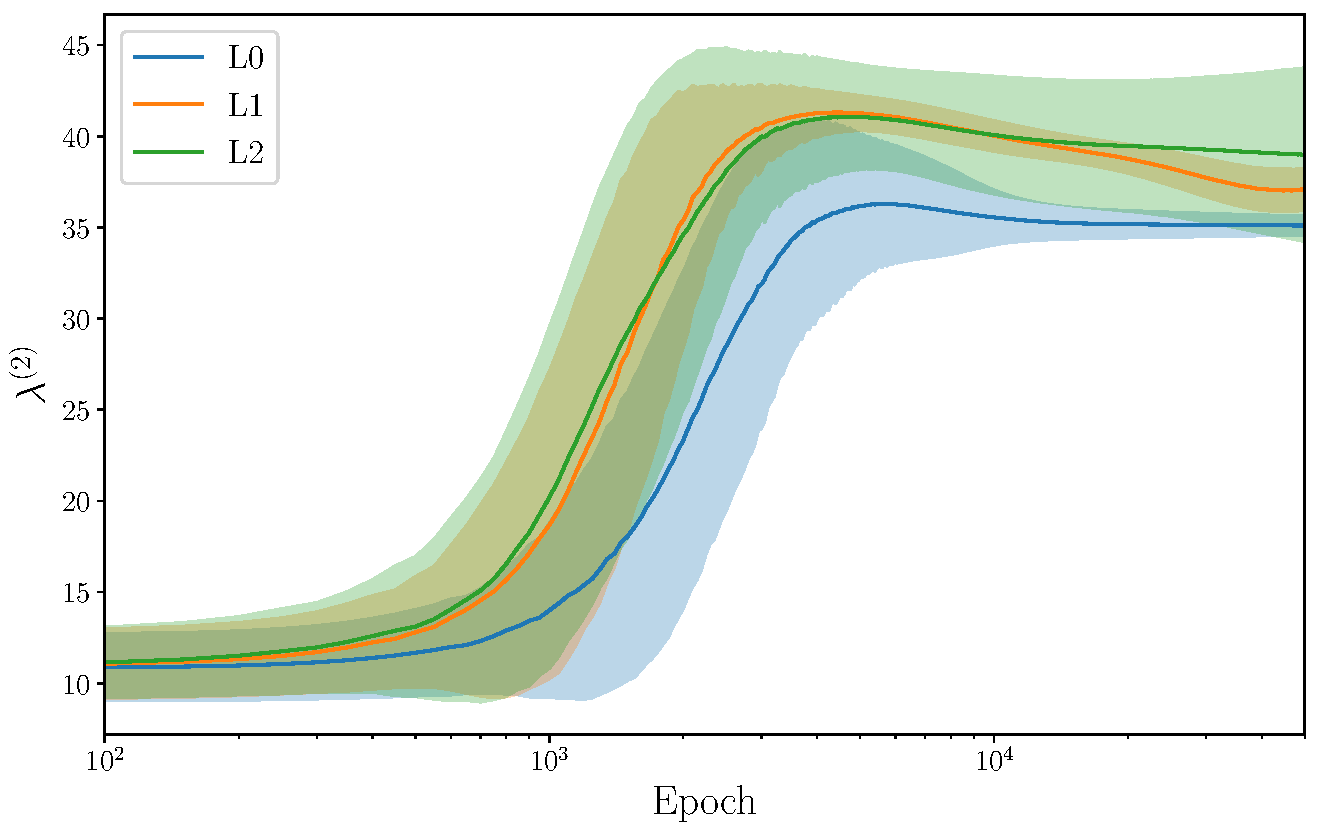
\includegraphics[width=0.30\textwidth]{figs/section_3/ntk_eigvals_L0_L1_L2_n_2.pdf}
  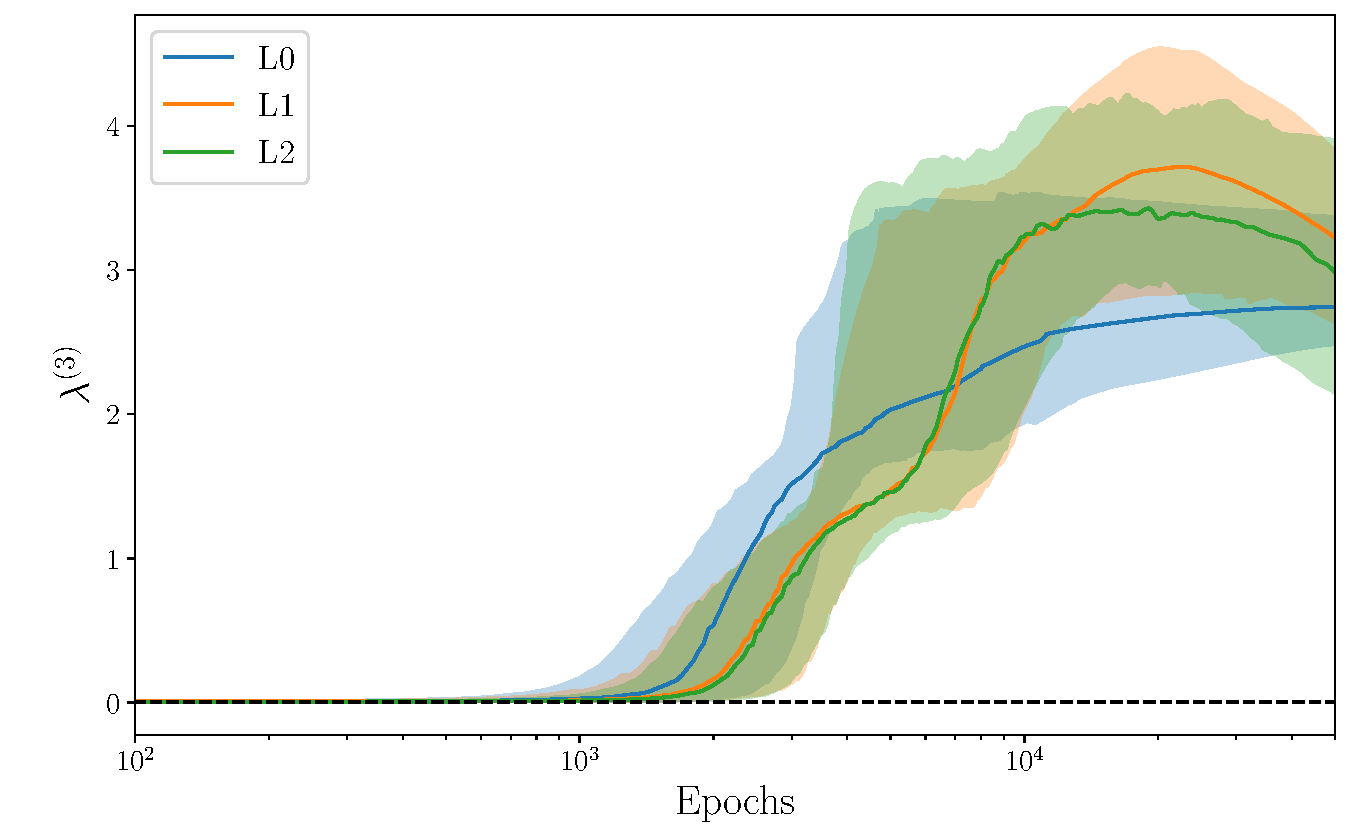
\includegraphics[width=0.30\textwidth]{figs/section_3/ntk_eigvals_L0_L1_L2_n_3.pdf}
  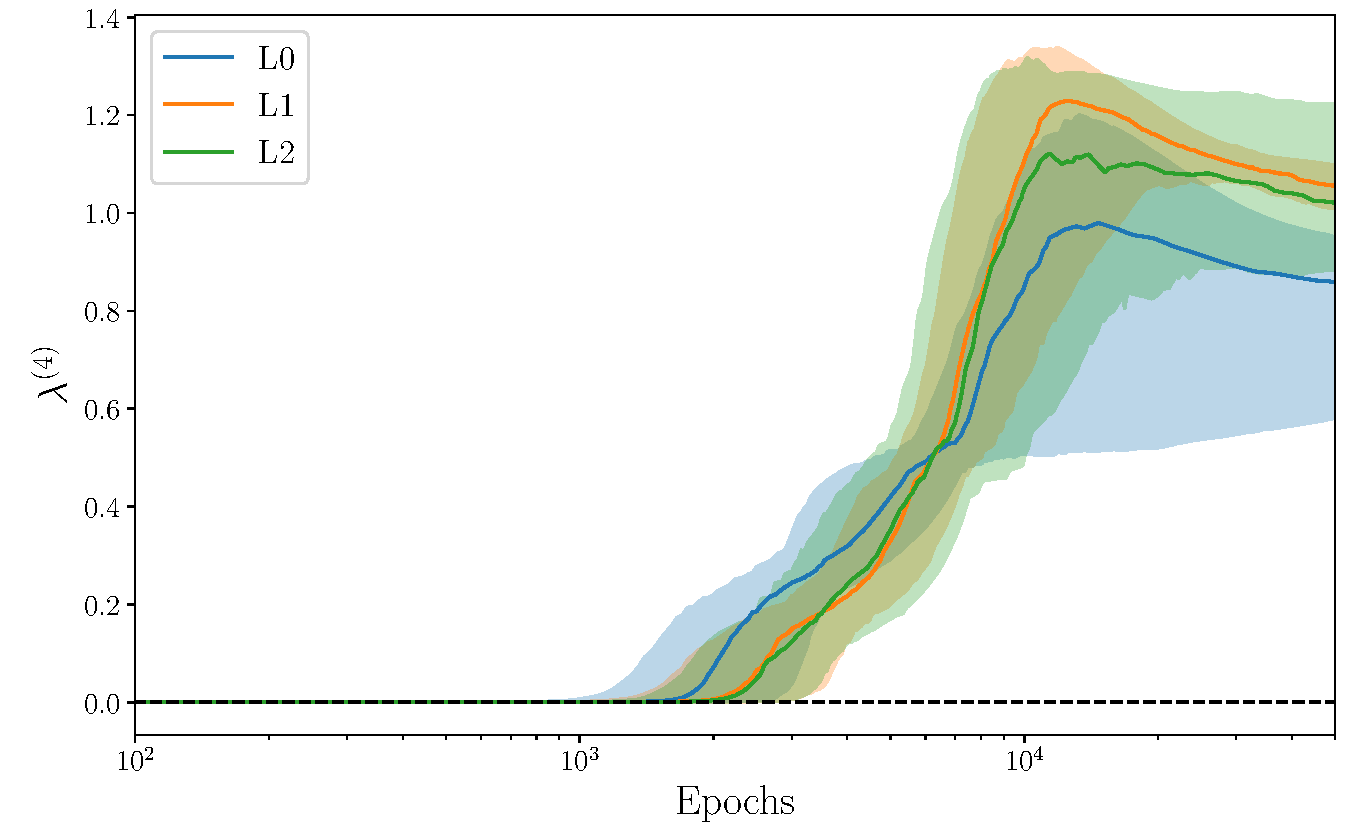
\includegraphics[width=0.30\textwidth]{figs/section_3/ntk_eigvals_L0_L1_L2_n_4.pdf}
  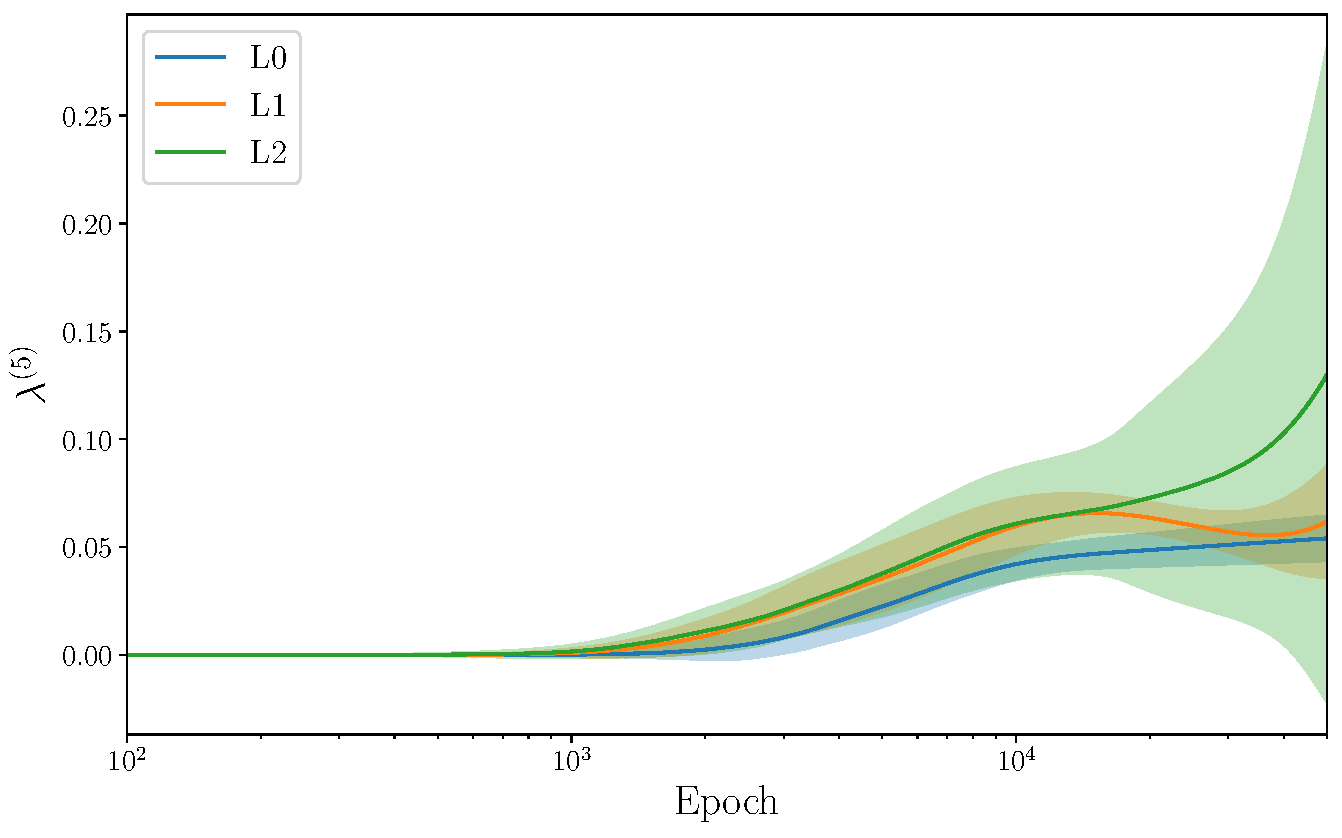
\includegraphics[width=0.30\textwidth]{figs/section_3/ntk_eigvals_L0_L1_L2_n_5.pdf}
  \caption{The first five eigenvalues of the NTK for L0, L1, and L2 data. Error
  bands correspond to one-sigma uncertainties over the ensemble of networks.}
  \label{fig:EigvalsComparison}
\end{figure}
% ===================================

In Fig.~\ref{fig:EigvalsComparison}, the same first five eigenvalues of the NTK
are displayed for L0, L1, and L2 data. We can make a few observations upon
inspecting these plots. First, we notice that the way in which data is generated
has an impact on the eigenvalues of the NTK. In general, the uncertainty bands
for L2 data are larger than those for L1 and L0 data, indicating that the NTK is
more sensitive to the noise in the data. This is consistent with the observation
made in Fig.~\ref{fig:NTKTime}. The eigenvalues reach a plateau and do not
change significantly once the network enters the lazy training regime. The
increase of the subdominant eigenvalues, combined with the analysis of
Eqs.~\eqref{eq:FlowParallel} and~\eqref{eq:FlowPerp}, suggests that more
``physical'' features become learnable before lazy training sets in.

% ===================================
\begin{figure}[t]
  \centering
  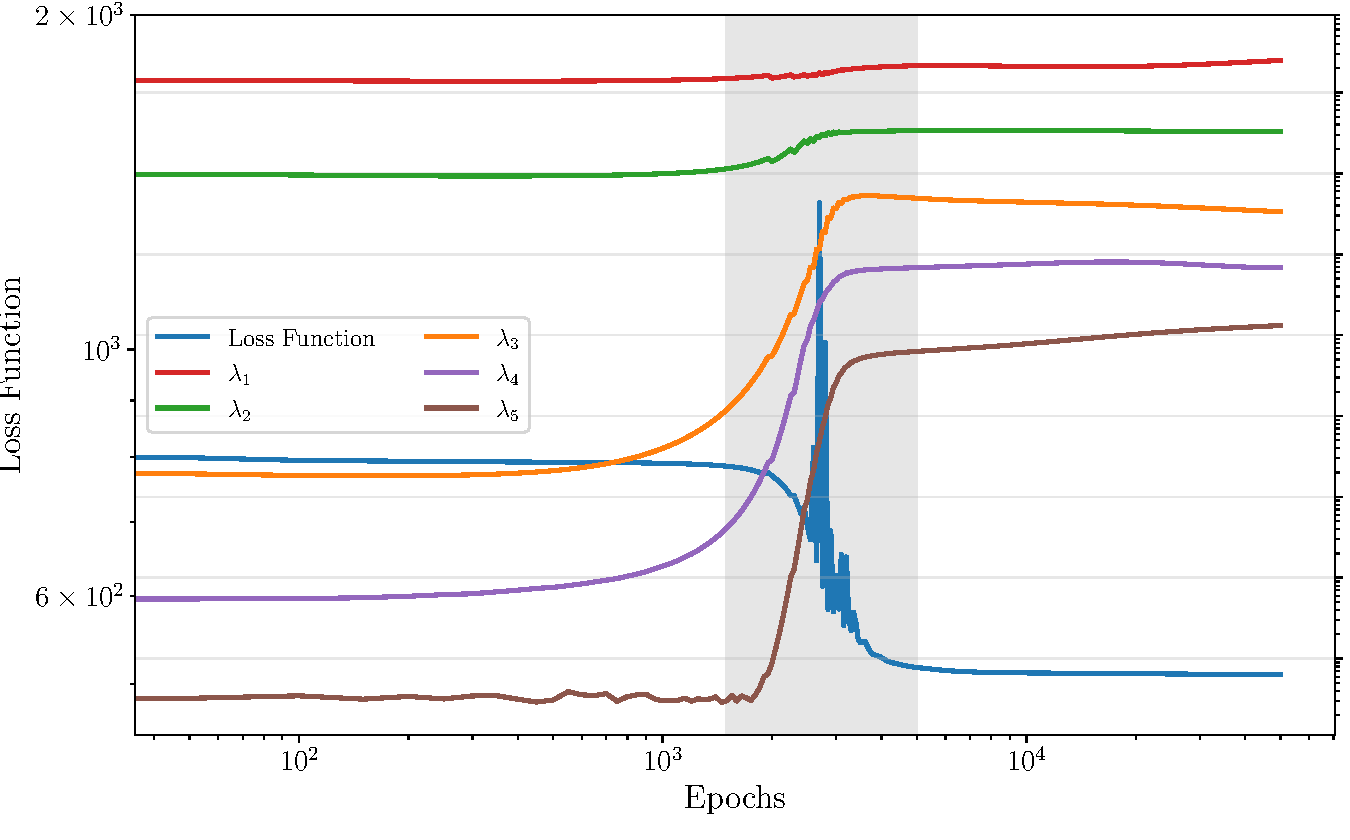
\includegraphics[width=0.45\textwidth]{section_3/loss_and_eigvals_vs_epochs.pdf}  
  \caption{Variation of the loss function overlaid with the first five
  eigenvalues for a selected replica over the ensemble. Left scale refers to the
  loss, while the right scale refers to the eigenvalues.}
  \label{fig:Loss}
\end{figure}
% ===================================

Finally, in Fig.~\ref{fig:Loss} we show the variation of the loss function
during training, overlaid with the first five eigenvalues of the NTK, for a
selected replica over the ensemble. It is interesting to see that in
correspondence with the sudden variation of the subdominant eigenvalues, the
loss function drops significantly, at the cost of an instability localised in
the descent. We interpret this as the network learning new features, changing
its internal representation to accommodate the new information. After this
initial phase, the eigenvalues stabilize and the loss function decreases
smoothly, as expected in the lazy training regime.

As it will be extensively discussed later in Sec.~\ref{sec:LazyTraining}, the
eigenvalues and eigenvectors of the NTK play a special role. Indeed, the output
$f$ can be decomposed into the basis of eigenvectors of the NTK. Hence the
eigenvectors corresponding to the larger eigenvalues can be interpreted as {\em
learnable}\ features, while the small (or zero) eigenvalues, correspond to
directions in which the field $f$ never evolves during training.

% \FloatBarrier

\subsubsection{Eigenvectors and Alignment of the NTK}
\label{sec:NTKAlign}

It has been argued before that there is a non-trivial interplay between the
eigenspace of the NTK and that of the matrix $M$. Indeed, the former encodes the
model dependence, while the latter brings physical information. Of course the
two matrices are independent at initialisation, and we do not expect any
alignment patter between the two. However, this picture does change during
training, as the NTK evolves and the model learns the target function. To
quantify this alignment, we define the matrix $A$, 
\begin{equation}
  \label{eq:MatrixA}
  A_{kk'} = \left( \left< z^{(k)}, v^{(k')}\right> \right)^2 = \cos^2(\theta_{kk'}) \;,
\end{equation}
where $z^{(k)}$ and $v^{(k')}$ are the $k$-th and $k'$-th eigenvectors of the
NTK and $M$, respectively. The matrix $A$ is thus a measure of the alignment
between the eigenspaces of the two matrices. The rows of the matrix correspond
to the eigenvectors of the NTK, ordered by the value of the corresponding
eigenvalues, with the eigenvectors corresponding to the larger eigenvalues at
the top of the matrix. The columns correspond to eigenvectors of the matrix $M$,
also ordered by the values of the corresponding eigenvalues, with the largest
eigenvalues to the left in this case. In Fig.~\ref{fig:NtkMAlign}, we show the
matrix $A$ at different epochs of the training for L2 data and a single NTK
replica. 
% ===================================
\begin{figure}[ht!]
  \centering
  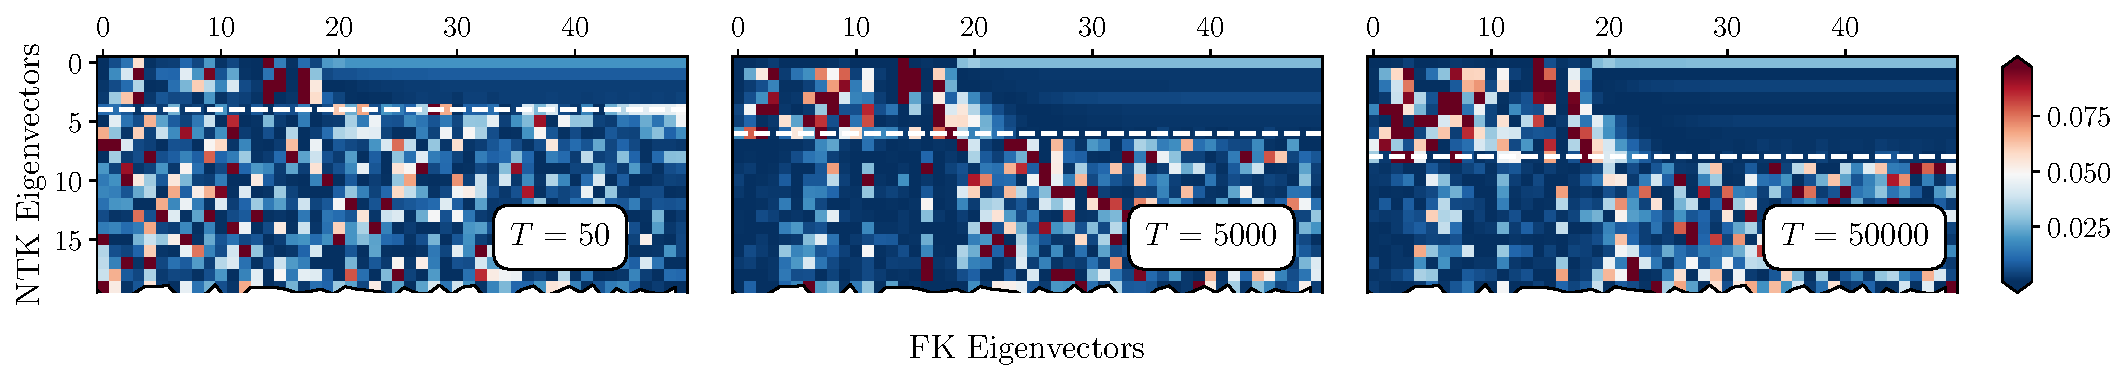
\includegraphics[width=1\textwidth]{section_3/ntk_alignment_L2.pdf}
  \caption{Matrix $A$ as defined in Eq.~\eqref{eq:MatrixA} for L2 data and for a
  single replica of the NTK. The matrix is shown at different epochs of the
  training process, indicated in the top of each panel. The white dashed line
  indicates the cut-off tolerance that we imposed to the eigenvalues of the NTK
  (see Appendix...?).}
  \label{fig:NtkMAlign}
\end{figure}
% ===================================

% ===================================
\begin{figure}[ht!]
  \centering
  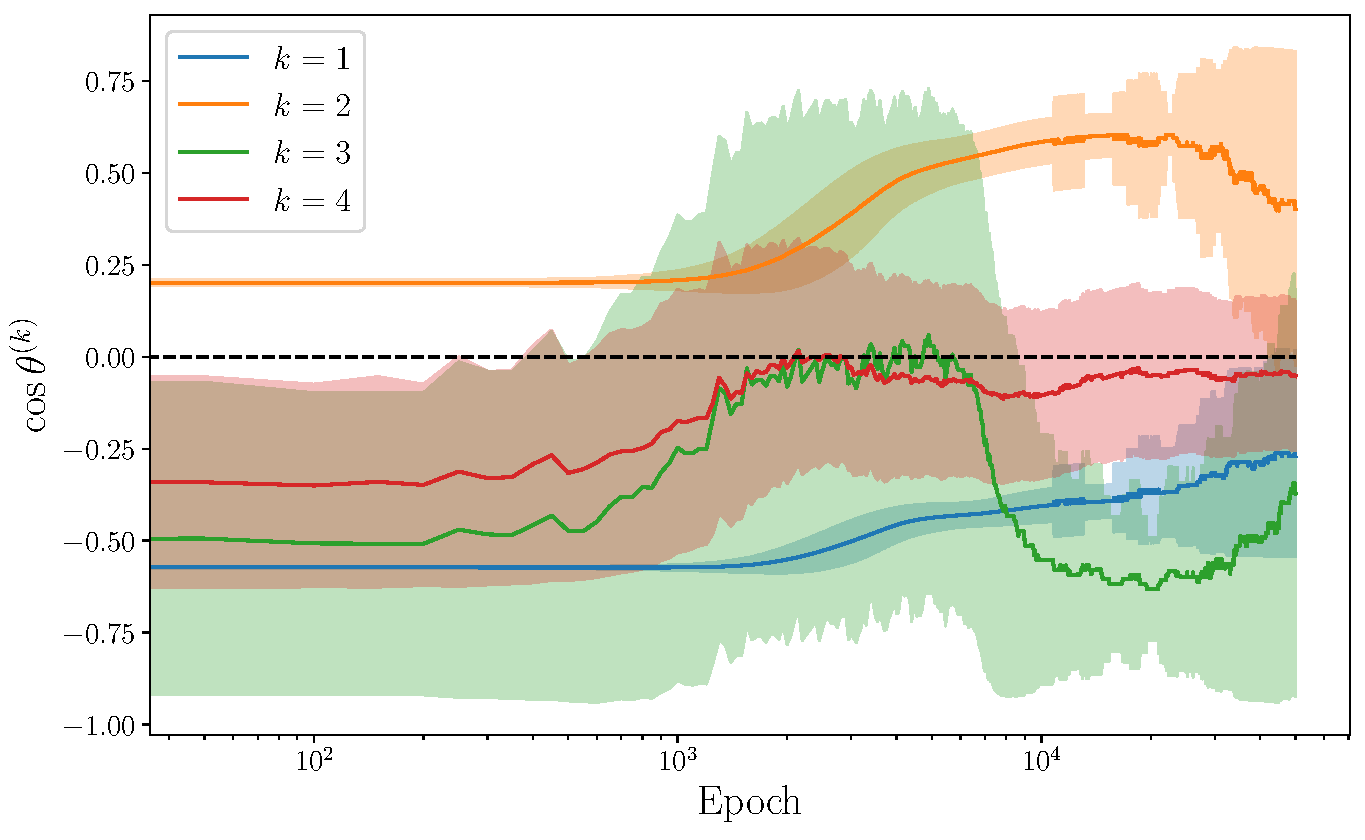
\includegraphics[width=0.45\textwidth]{section_3/ntk_alignment_fin_L2_1}
  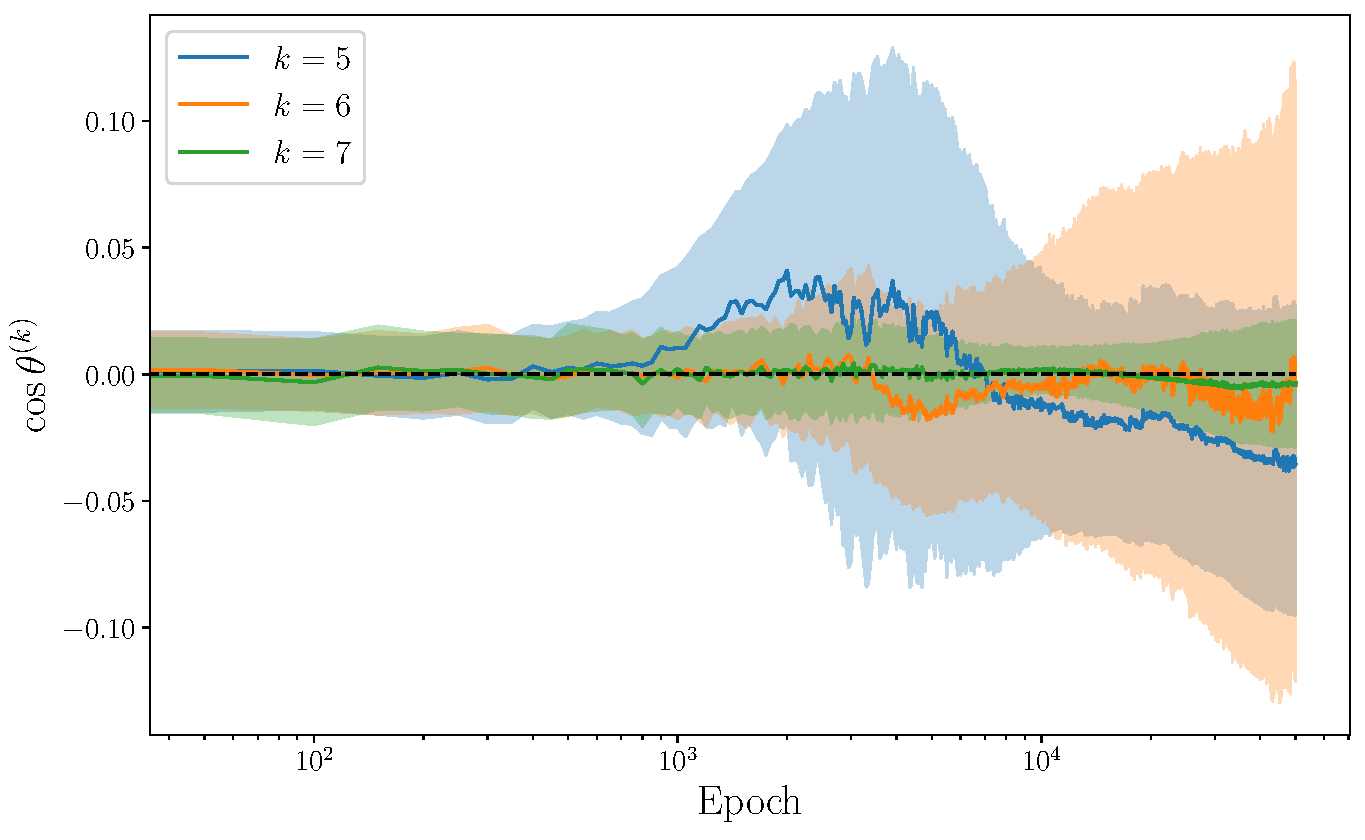
\includegraphics[width=0.45\textwidth]{section_3/ntk_alignment_fin_L2_2}
  \caption{Alignment of the eigenvectors of the NTK with the input function
  $f^{\rm(in)}$ used to generate the L2 data, measured in terms of $\cos
  \theta^{(k)} = (z^{(k)}, f^{\rm{(in)}})/ \Vert f^{\rm{(in)}}\Vert$. In the
  left panel, the first five eigenvectors of the NTK are shown, while the right
  panel shows the remaining eigenvectors up to $k=7$.}
  \label{fig:NTKAlignFin}
\end{figure}
% ===================================
% ===================================
\begin{figure}[ht!]
  \centering
  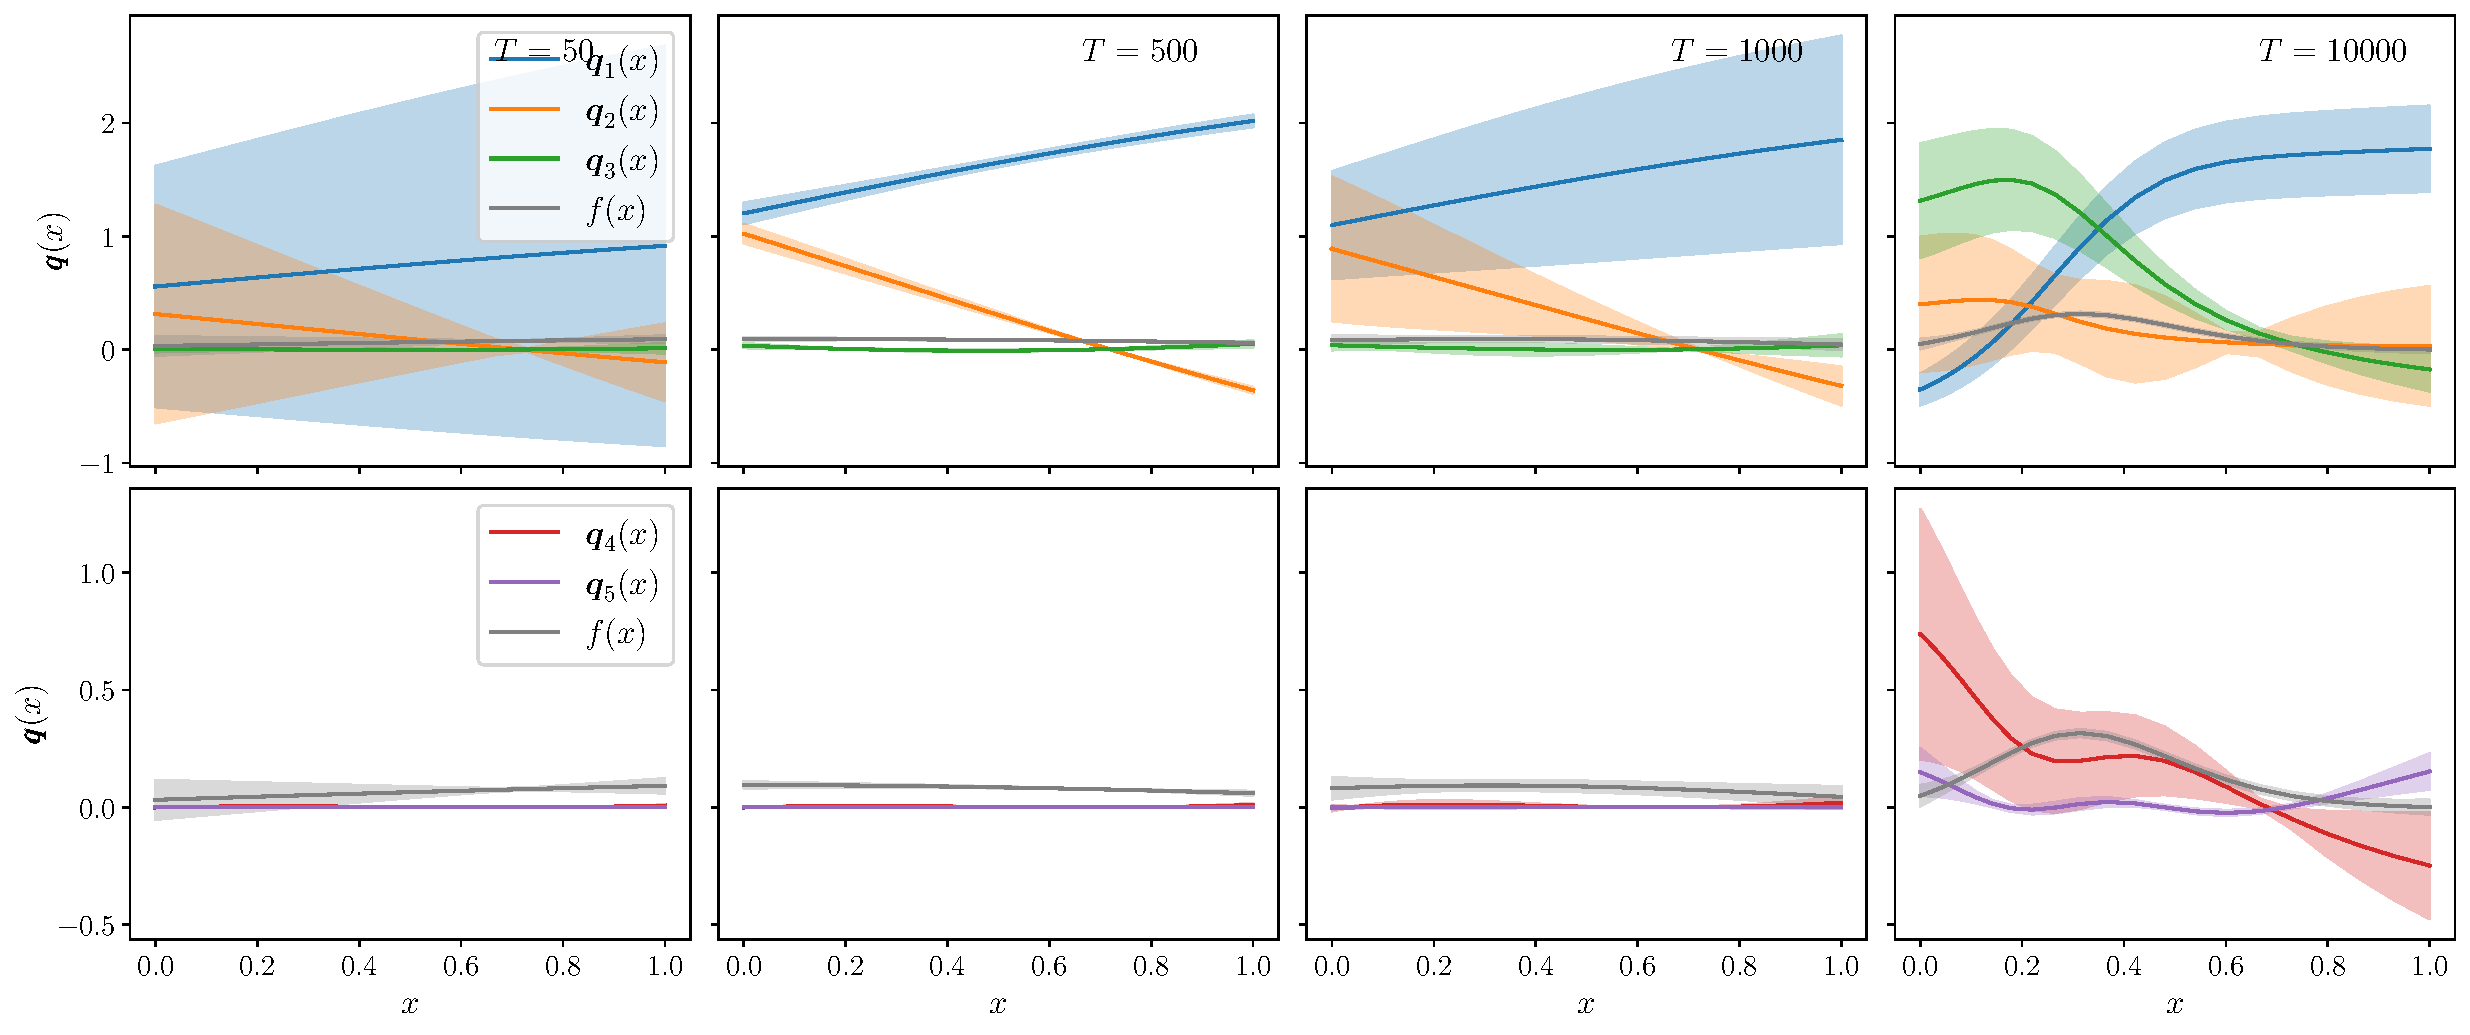
\includegraphics[width=0.90\textwidth]{section_3/q_directions_sign.pdf}
  \caption{First five eigenvectors of the combined matrix $H=\Theta M$, as in
  Eq.~\eqref{eq:FlowEquationNoIndices}, at different training time and as
  function of the input $x$-grid. We also show the output of the network at the
  same training time, which is displayed in gray.}
  \label{fig:NTKMEigVecs}
\end{figure}
% ===================================

The blue rectangle in the top right corner of the matrix shows that the
eigenvectors of the NTK corresponding to the largest eigenvalues are orthogonal
to the eigenvectors of $M$ that are in the kernel of $M$, \ie\ the directions
that do not contribute to the observables. It is useful to remember that the
largest eigenvalues of the NTK correspond to the directions that are orthogonal
to $\ker\Theta$, \ie\ the directions that are learnable during the training
process. In order to have a robust training process, we expect these learnable
directions to align with the directions that actually contribute to the loss
functions, \ie\ the ones corresponding to the largest eigenvalues of $M$.
Consistently with this intuition, we see that the size of this blue rectangle
increases with training time. In particular, it is clear from our plot that it
becomes deeper by the onset of the lazy training regime: more of the learnable
directions -- the {\it features}\ that the network can learn -- are aligned with
the directions that contribute most to the observables.

A similar analysis can also be performed by studying the alignment of the
eigenvectors of the NTK with the input function used to generate the data. In
Fig.~\ref{fig:NTKAlignFin}, we show the cosine of the angle between the two
vectors for two subsects of eigenvectors, in the right and left panel
respectively. In these two plots, different pattern can be observed. First, the
first four angles vary considerably during training. These observations lead us
to conclude that other than changing the dominant eigenvectors, the NTK is also
activating some others that were asleep in the first stage of training. This in
accordance to what has been previously observed in
Figs.~\ref{fig:EigvalsComparison}-\ref{fig:NtkMAlign}. 

A complementary picture is displayed in Fig.~\ref{fig:NTKMEigVecs}. Here, we
show the eigenvectors of the matrix $H = \Theta M$, labelled with $q^{(i)}$, at
different training times and as functions of the $x$-grid. Together with the
eigenvectors, we also show the output of the trained neural network at the
corresponding training time. From these plots, we see that as the training
progress, the shape of the eigenvectors become more structured in order to
reproduce the output function. Again, this conclusion supports the observations
made previously in various occasions, that during training the neural network is
changing its internal representation and the NTK encodes this information.

\FloatBarrier

\section{Lazy Training in NNPDF}
\label{sec:LazyTraining}

In the previous section we presented an empirical study of the training dynamics
through the lens of the NTK. We observed that the NTK is able to capture the
main features of the training process, and that its time evolution is
characterised by a rapid initial transient, followed by a slower evolution
during the rest of the training. We now turn our attention on this last stage of
the training, where the NTK has stabilised and becomes approximately constant.
In doing so, we will build upon the results presented in
Refs.~\cite{jacot2018neural,lee2019wide} and extend them to the case of NNPDF.
In the following, we derive the analytical solution of the flow equation, which
allows us to write an explicit expression for the trained field as a function of
the field at initialisation and the data.

\subsection{Solution of the Flow Equation}
\label{sec:Lazy}

The lazy training regime is characterised by a slow-evolving NTK. We denote as
$T_{\rm ref}$ the time at which the onset of this regime occurs. The NTK is then
\textit{frozen} to its value at $T_{\rm ref}$, and from this time onward the NTK
is taken to be constant
\begin{equation}
  \Theta_t = \Theta_{T_{\rm ref}} \equiv \Theta, \quad \textrm{for } t \geq T_{\rm ref}.
\end{equation} 
The flow equation can then be written as
\begin{align}
  \ddt f_t = -\Theta M f_t + b\, ,
  \label{eq:FlowEqTwo}
\end{align}
where $M$ and $b$ are defined as in Eq.~\eqref{eq:MandBDef}. Note that now
neither $\Theta$ nor $b$ depend on the training time $t$. In order to solve this
first-order linear differential equation, we observe that the eigenvectors of
$\Theta$,
\begin{align}
    \label{eq:ThetaEigensystem}
    \Theta z^{(k)} = \lambda^{(k)} z^{(k)}\, ,
\end{align}
provide a basis for expanding Eq.~\eqref{eq:FlowEqTwo}. Furthermore, owing to
the spectrum hierarchy of the NTK (Fig.~\ref{fig:NTKEigvalsTime}), it is
necessary to distinguish the components of $f_t$ that are in the kernel of
$\Theta$ from the ones that are in the orthogonal complement. We introduce the
notation
\begin{align}
    \label{eq:ParallelCompnents}
    &f^\parallel_{t,k} = \left(z^{(k)}, f_t\right)\, , \quad \text{if}\ \lambda^{(k)} = 0\, , \\
    \label{eq:OrthogonalComponents}
    &f^\perp_{t,k} = \frac{1}{\sqrt{\lambda^{(k)}}} \left(z^{(k)}, f_t\right)\, , \quad
        \text{if}\ \lambda^{(k)} \neq 0\, ,
\end{align}
where the scalar product has been defined as
\begin{equation}
  \left(f'_{t'}, f_t\right) = \sum_{i,\alpha} f'_{t',i\alpha} f_{t,i\alpha}\,.
\end{equation}
One can readily see that the components in the kernel of $\Theta$, $\text{ker}\
\Theta$, do not evolve during training,\footnote{Despite this result having been
obtained using the frozen NTK, it is worth mentioning that at any time during
training the kernel of the NTK is always defined and in general non-empty.
Hence, also in the initial stage, there will be a component that is completely
determined by the initial condition, \ie\ by the prior distribution in functional
space.}
\begin{align}
    \label{eq:FlowParallel}
    \ddt f^\parallel_{t,k} = 0
        \quad \Longrightarrow \quad f^\parallel_{t,k} = f^\parallel_{0,k}\, .
\end{align}
This means that the final solution will be affected by an irreducible noise that
is purely dictated by the initial condition. 

The flow equation for the orthogonal components can be written as
\begin{align}
    \label{eq:FlowPerp}
    \ddt f^\perp_{t,k} = - H^\perp_{kk'} f^\perp_{t,k'}
        + B^\perp_{k}\, ,
\end{align}
where  we introduced
\begin{align}
    H^\perp_{kk'} &= \sqrt{\lambda^{(k)}} \left(z^{(k)}, M z^{(k')}\right) \sqrt{\lambda^{(k')}}\, ,\\
    B^\perp_k &= -\sqrt{\lambda^{(k)}} \left[\left(z^{(k)}, M z^{(k')}\right) f^\parallel_{0,k'}
        - \left(z^{(k)}, \FKtabT C_Y^{-1} Y\right)\right]\, .
\end{align}
As discussed above, the indices on quantities that have a $\perp$ suffix only span the space
orthogonal to the kernel of $\Theta$, while the indices on quantities that have
a $\parallel$ suffix span the kernel. We refer to $H^\perp$ as the flow (or
training) Hamiltonian, training can only take place in the space orthogonal
to the kernel of $\Theta$; we see explicitly in the definition above that the flow
dynamics is determined by a combination of the architecture of the NN, encoded
in the NTK, and the data, on which $M$ depends. More specifically, the matrix
elements of $M$ can be written as
\begin{align}
    \label{eq:MMatElems}
    \left(z^{(k)}, M z^{(k')}\right) = T^{(k)T} C_Y^{-1} T^{(k')}\, ,
\end{align}
where $T^{(k)} = T[z^{(k)}]$ is the vector of theory predictions for the data
obtained using $z^{(k)}$ as the input PDF. Similarly, we have
\begin{align}
    \label{eq:BMatElems}
    \left(z^{(k)}, \FKtabT C_Y^{-1} Y\right) = T^{(k)T} C_Y^{-1} Y\, .
\end{align}
Denoting by $d^\perp$ the dimension of the subspace orthogonal to $\text{ker}\
\Theta$, $H^\perp$ is a $d^\perp\times d^\perp$ symmetric matrix, whose
eigenvalues and eigenvectors satisfy
\begin{align}
    H^\perp_{kk'} w^{(i)}_{k'} = h^{(i)} w^{(i)}_{k}\, .
\end{align}
The solution to Eq.~\eqref{eq:FlowPerp} can be written as the sum of the
solution of the homogeneous equation, $\hat{f}^{\perp}_{t,k}$, and a particular
solution of the full equation. The solution of the homogeneous equation is
\begin{align}
    \label{eq:HomoSoln}
    \hat{f}^{\perp}_{t,k} = \sum_{i=1}^{d^\perp} f^{\perp}_{0,i} e^{-h^{(i)}t} w^{(i)}_k\, ,
\end{align}
where
% ~\footnote{ Note that here the scalar product is computed in the subspace
%     orthogonal to the kernel of $\Theta$,
%     \[
%         \left(w^{(i)}, f^\perp_0\right) = \sum_{k=1}^{d_\perp} w^{(i)}_{k} f^\perp_{0,k}
%     \]
% }
\begin{align}
    \label{eq:InitialCi}
    f^{\perp}_{0,i} = \sum_{k=1}^{d_\perp} w^{(i)}_k f^\perp_{0,k}\, ,
        %= \left(w^{(i)}, f^\perp_0\right)\, ,
\end{align}
guarantees that the initial condition $\hat{f}^\perp_{t,k}=f^\perp_{0,k}$ is
satisfied. Similarly, if we define
\begin{align}
    \label{eq:BiDef}
    \Upsilon^{(i)} = \sum_{k=1}^{d_\perp} w^{(i)}_k B^\perp_{k}\, ,
        %= \left(w^{(i)}, B^\perp\right)\, ,
\end{align}
then
\begin{align}
    \label{eq:PartSol}
    \check{f}^\perp_{t,k} = \sideset{}{'}\sum_{i} \frac{1}{h^{(i)}} \Upsilon^{(i)}
        \left(1 - e^{-h^{(i)}t}\right) w^{(i)}_k\, ,
\end{align}
where the sum only involves the non-zero modes of $H^\perp$, is a particular
solution of the inhomogeneous equation, which satisfies the boundary condition
$\check{f}^{\perp}_{0,k}=0$. Finally, the solution of the flow equation in the
subspace orthogonal to $\text{ker}\ \Theta$ is
\begin{align}
    f^\perp_{t,k}
    \label{eq:FlowSolution}
        &= \hat{f}^\perp_{t,k} + \check{f}^\perp_{t,k}
        % &= \sum_{i=1}^{d^\perp}  \left(w^{(i)}, f^\perp_0\right) e^{-h^{(i)}t} w^{(i)}_k
        %     + \sideset{}{'}\sum_{i=1}  \frac{1}{h^{(i)}} \left(w^{(i)}, B^\perp\right)
        %         \left(1 - e^{-h^{(i)}t}\right) w^{(i)}_k
        \, .
\end{align}
Finally, collecting the parallel contribution, Eq.~\eqref{eq:FlowParallel}, and
the solution of the orthogonal component, Eq.~\eqref{eq:FlowSolution}, yields a
simple expression,
\begin{align}
    \label{eq:AnalyticSol}
    f_{t,\alpha}
        = U(t)_{\alpha\alpha'} f_{0,\alpha'} + V(t)_{\alpha I} Y_{I}\, .
\end{align}
The two evolution operators $U(t)$ and $V(t)$ have lengthy, yet explicit,
expressions, which we summarise here: 
\begin{align}
    U(t)_{\alpha\alpha'} = \hat{U}^\perp(t)_{\alpha\alpha'}
        + \check{U}^\perp(t)_{\alpha\alpha'} + U^\parallel_{\alpha\alpha'}\, ,
\end{align}
where
\begin{align}
    \hat{U}^\perp(t)_{\alpha\alpha'}
        = \sum_{k,k'\in\perp} \sqrt{\lambda^{(k)}} z^{(k)}_\alpha 
            \left[\sum_i w^{(i)}_{k} e^{-h^{(i)}t} w^{(i)}_{k'}\right]
            z^{(k')}_{\alpha'} \frac{1}{\sqrt{\lambda^{(k')}}}\, ,
\end{align}
and
\begin{align}
    U^\parallel_{\alpha\alpha'}
        = \sum_{k''\in\parallel} z^{(k)}_\alpha z^{(k)}_{\alpha'} \, .
\end{align}
The contributions from $\check{U}^\perp(t)$ and $V(t)$ are more easily expressed
by introducing the operator
\begin{align}
    \label{eq:MOperatorDef}
    \mathcal{M}(t)_{\alpha\alpha'} 
        = \sum_{k,k'\in\perp} \sqrt{\lambda^{(k)}} z^{(k)}_\alpha 
            \left[\sideset{}{'}\sum_{i} w^{(i)}_{k} \frac{1}{h^{(i)}}\, 
            \left( 1- e^{-h^{(i)}t}\right) w^{(i)}_{k'}\right]
            z^{(k')}_{\alpha'} \sqrt{\lambda^{(k')}}\,. 
\end{align}
Then, we can write
\begin{align}
    \label{eq:UperpCheck}
    \check{U}^\perp(t)
        = - \mathcal{M}(t)\; \FKtabT C_Y^{-1} \FKtab 
            \left[\sum_{k''\in\parallel} z^{(k'')} z^{(k'') T}\right]\, ,
\end{align}
and
\begin{align}
    V(t) = \mathcal{M}(t)\; \FKtabT C_Y^{-1}\, ,
\end{align}
where we note that the term in the bracket in Eq.~\eqref{eq:UperpCheck} is
simply the projector on the kernel of the NTK. The four terms that appear in the
analytical solution have a clear physical interpretation:
\begin{itemize}
    \item The first term $\hat{U}^\perp(t)$ suppresses the components of the
    initial condition that lie in the subspace orthogonal to the kernel of the
    NTK. These are the components that are learned by the network during
    training. While the trained solution still depends on its value at
    initialisation, that dependence is suppressed during training. This
    suppression is exponential in the training time, and the rates are given by
    the eigenvalues of $H^{\perp}$.
    \item The contribution from $U^\parallel$ yields the component of the
    initial condition that lies in the kernel of the NTK. As such, those
    components remain unchanged during training and are part of the trained
    field at all times $t$. 
    \item The two remaining contributions are best understood by combining them
    together,
    \begin{align}
        \label{eq:DataCorrectedInference}
        \check{U}^{\perp}(t) f_{0} + V(t) Y 
            = \mathcal{M}(t)\; \FKtabT C_Y^{-1} \left[Y - \FKtab f_{0}^{\parallel}\right]\, .
    \end{align}
    The parallel component of the initial condition $f_{0}^{\parallel}$ does not
    evolve during training, and therefore it yields a contribution $\FKtab
    f_{0}^{\parallel}$ to the theoretical prediction of the data points at all
    times $t$. This is taken into account by subtracting this contribution from
    the data, before the inference is performed.
\end{itemize}

% Onset Lazy L2 ===================================
\begin{figure}[t]
  \centering
  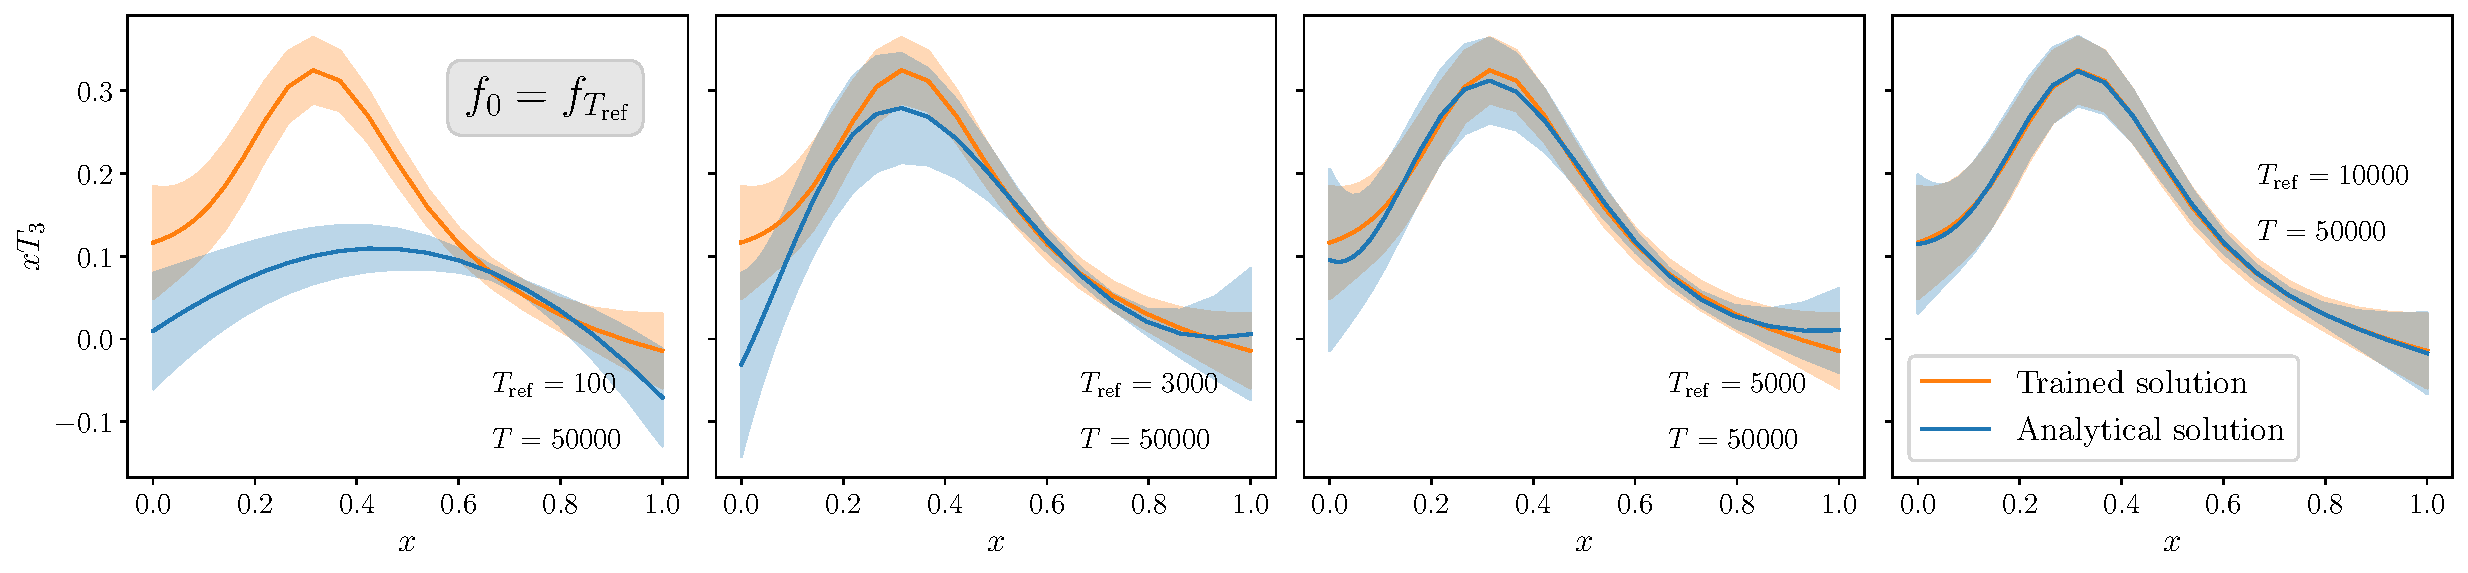
\includegraphics[width=0.9\textwidth]{section_4/evolution_vs_trained_ftref_L2.pdf} 
  \caption{Comparison of the trained and analytical evolution at the end of
  training. Each panel corresponds to a different frozen NTK, whereby the
  analytical solution is computed starting from $f_{T_{\rm Ref}}$. The orange
  curve represents the final trained function after 50000 iterations of GD, and
  is the same across panels. Error bands represent one-sigma uncertainties
  across replicas. L2 data is used.}
  \label{fig:OnsetLazyL2}
\end{figure}
% =================================================
The solution in Eq.~\eqref{eq:AnalyticSol} is the main result of this section.
It shows that the training process can be described as the sum of a linear
transformation of the initial fields $f_{0,\alpha}$, and a linear transformation
of the data $Y_I$. The two transformations depend on the flow time $t$ and are
given by the evolution operators $U(t)$ and $V(t)$. Fig.~\ref{fig:OnsetLazyL2}
compares the analytical solution with the trained function at the end of
training, for different choices of the frozen NTK. The evolution time $T$ used
in the analytical solution is the difference between the total training time and
$T_{\rm ref}$. Central value and uncertainty bands are obtained by computing the
analytical solution for each replicas of the initial condition and frozen NTK.
\footnote{
  If not stated otherwise, in this section central values and uncertainties are
  always computed as ensemble averages across replicas.
}
The figures agree with the expectation; the closer $T_{\rm ref}$ is to the
onset of the lazy regime, the better the agreement between the analytical
solution and the trained function.

A complementary perspective is provided in Fig.~\ref{fig:FrefDecompositionL2},
where the analytical solution is decomposed into the two contributions from $U$
and $V$. In each panel, the initial condition $f_{T_{\rm ref}}$ is evolved
analytically for different training times by keeping the frozen NTK fixed. We
see that as training proceeds, the contribution from $U$ is progressively
suppressed, in accordance with the observation made above. On the other hand,
the contribution from $V$ grows and becomes dominant at later epochs, indicating
that the trained function is mostly determined by the data, rather than the
previous condition of the network. We also observe that such behaviour happens
quite rapidly, as a consequence of the fact the time scales in the analytical solution are
determined by the inverse of the eigenvalues of $H^\perp$, and latter 
are typically large.
% Decomposition L2 ================================
\begin{figure}[ht]
    \centering
    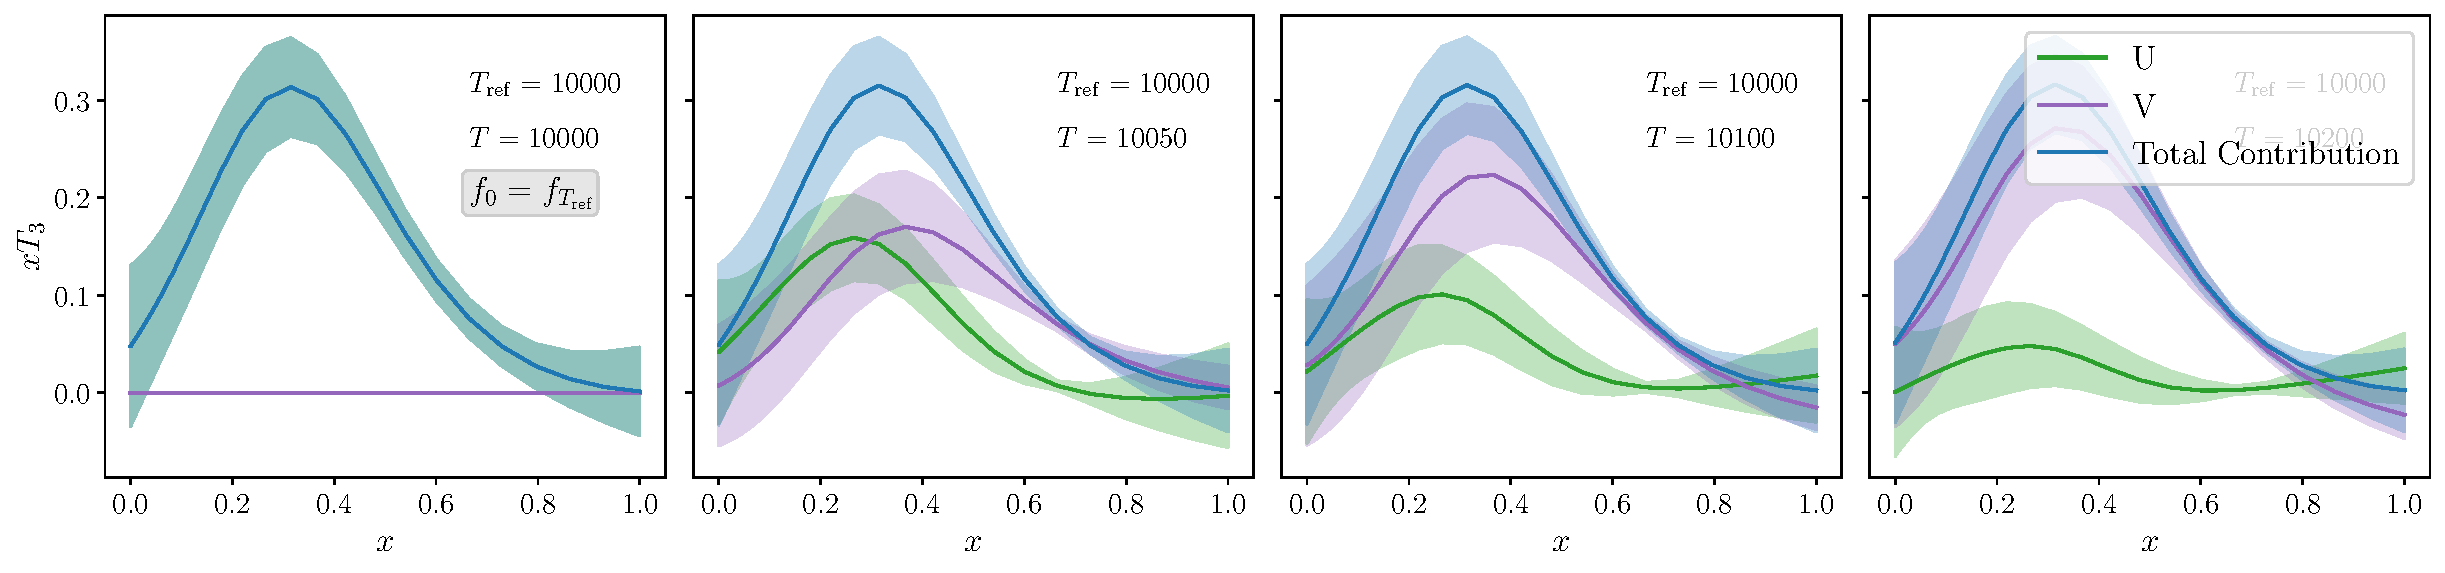
\includegraphics[width=0.9\textwidth]{section_4/u_v_decomposition_L2.pdf} 
    \caption{Decomposition of the analytical solution into the two contributions
    from $U$ and $V$ at different training times. The frozen NTK is fixed across
    panels, and corresponds to the one at $T_{\rm ref} = 10000$. The initial
    condition is always $f_{T_{\rm ref}}$. As in Fig.~\ref{fig:OnsetLazyL2}, L2 data
    is used.}
    \label{fig:FrefDecompositionL2}
  \end{figure}
  % =================================================
  
  
The analytical solution in Eq.~\eqref{eq:AnalyticSol} sheds a new light onto the
behaviour of the numerical training of a neural network. Given these results, it
is natural to ask whether the information encoded in the NTK alone can drive
training beyond its original initial condition, \ie\ whether the analytical
solution can be used to perform kernel learning. We address this question in the
following section.

\subsection{Lazy Training as Kernel Learning}
\label{sec:NTKKernelLearning}

The results shown in Sec.~\ref{sec:Lazy} and Sec.~\ref{sec:NTKDuringTraining}
support the idea that the NTK is capable to encode in its eigenvectors 
the physical features learned
during training. We now probe this idea further by employing the analytical
solution in Eq.~\eqref{eq:AnalyticSol} \textit{\`a la} kernel learning, \ie\ by
applying it to an initial condition that represents our prior. In the following,
we choose the initial condition to be an ensemble of networks at initialisation
as in Fig.~\ref{fig:prior}, whose architecture is the same as the one used in
the training. This represents our prior assumption on the space of functions,
which is then updated using the data and the NTK frozen at $T_{\rm ref}$.

\subsubsection{Convergence of the Analytical Solution}
% Grid plot with L2 ================================
\begin{figure}[t]
  \centering
  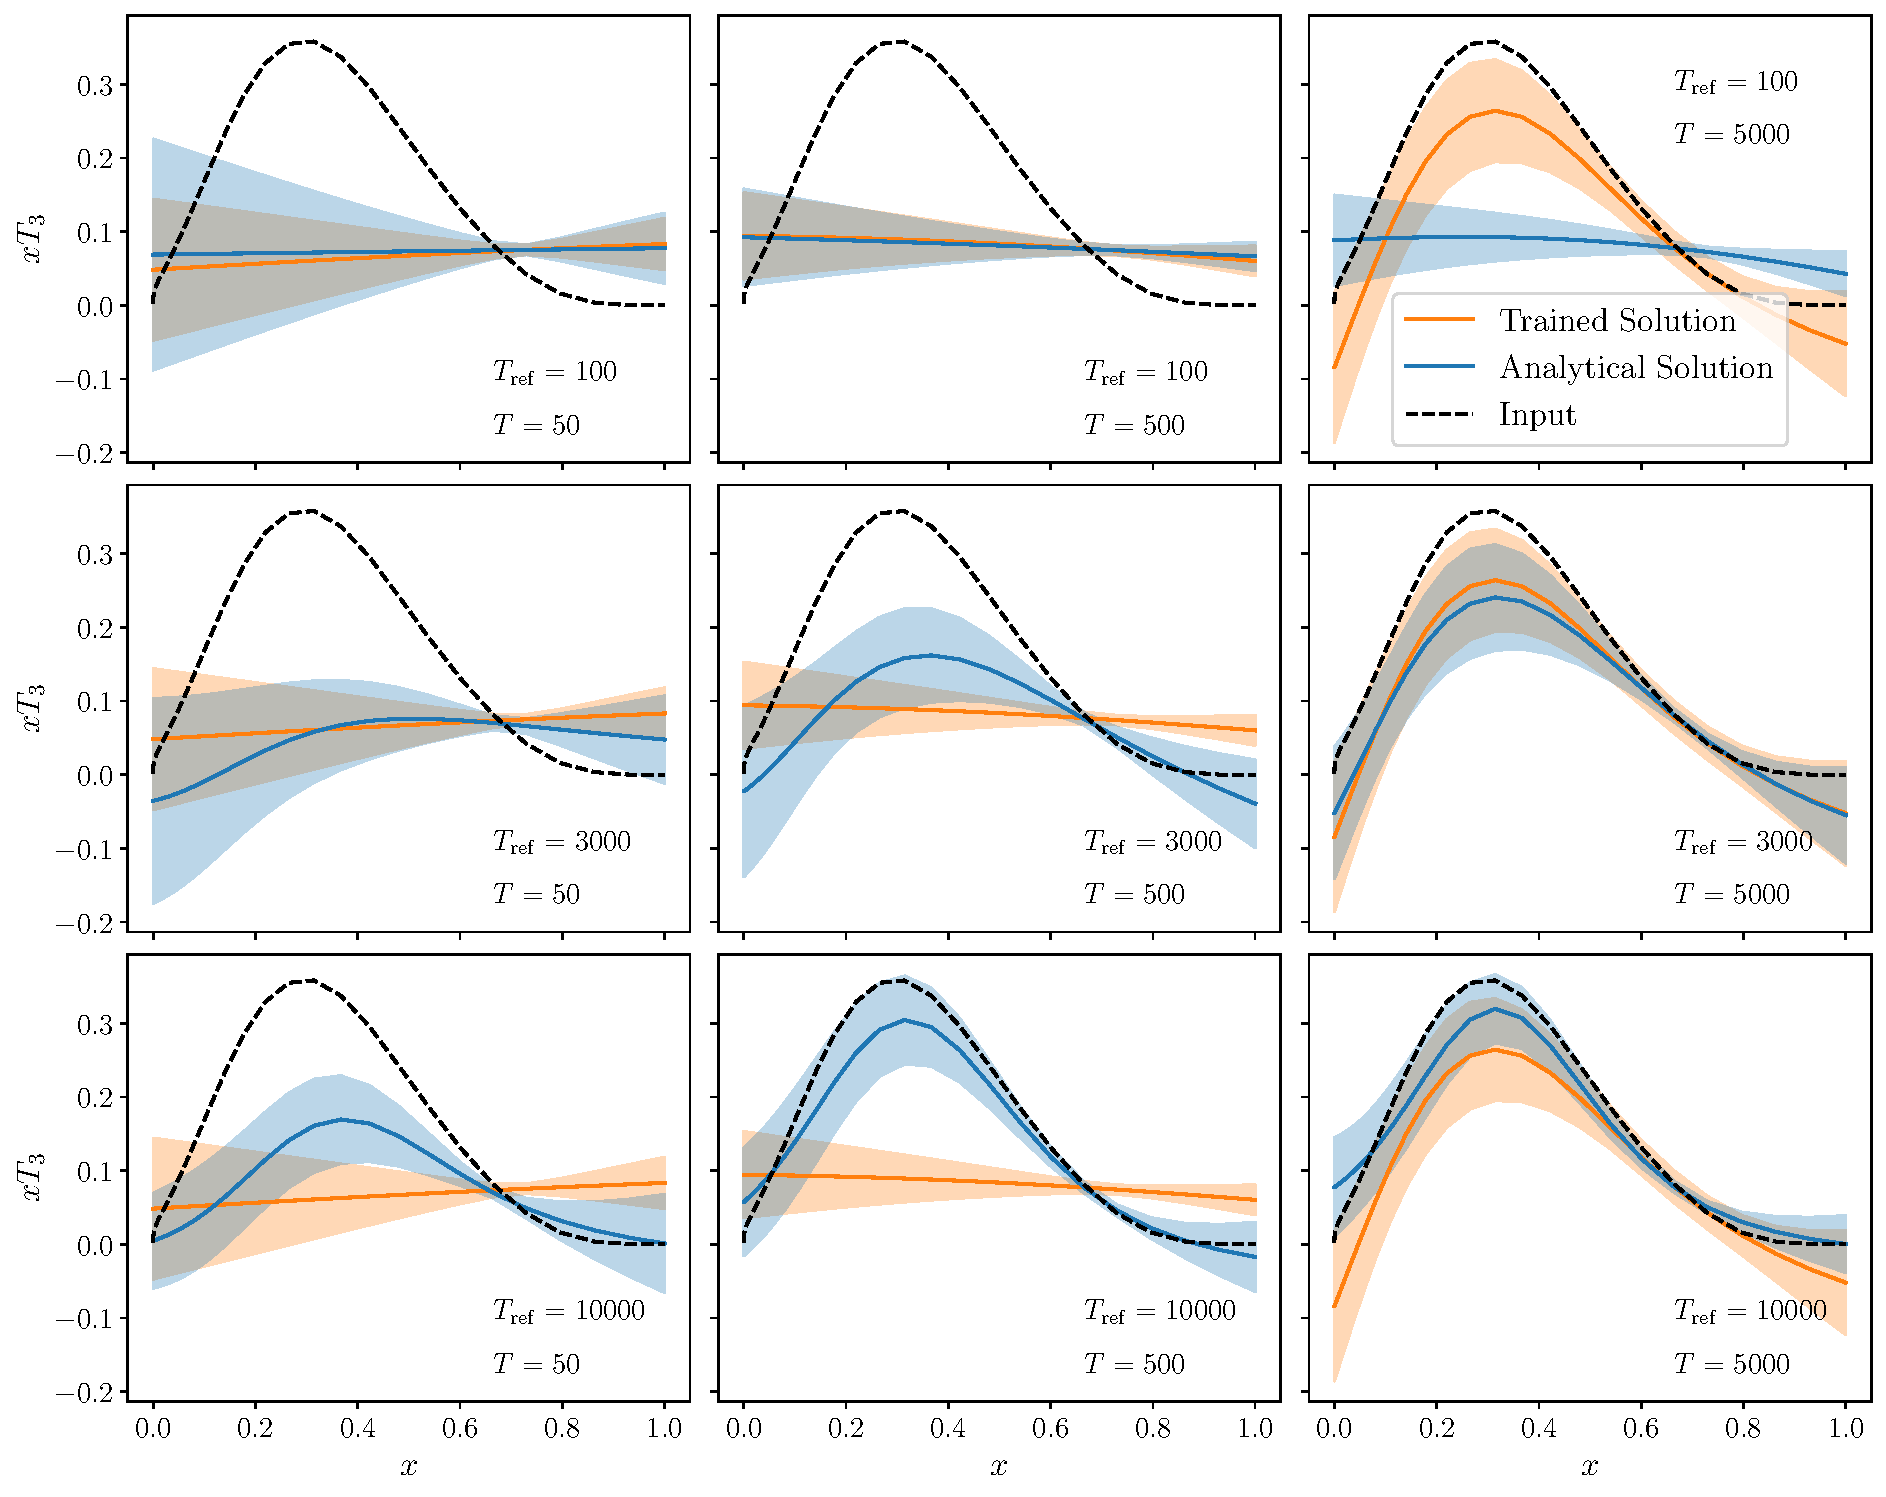
\includegraphics[width=0.9\textwidth]{section_4/evolution_f0_vs_trained_grid_L2.pdf} 
  \caption{Comparison of the trained (orange) and analytical (blue) evolution
  starting from an ensemble of networks at initialisation as the initial
  condition. Each row corresponds to a different frozen NTK, while the columns
  represent different training times. L2 data is used.}
  \label{fig:EvolutionGridF0L2}
\end{figure}
% =================================================
We start by comparing the analytical solution (AS), obtained using an ensemble
of networks at initialisation as the initial condition, with the trained
solution (TS), obtained after training a neural network from a different initial
condition. This comparison is shown in Fig.~\ref{fig:EvolutionGridF0L2} for L2
data, where the rows in the grid correspond to different frozen NTKs, while the
columns represent numerical and analytical evolution after $T=50, 500$ and 5000
epochs. These results deserve a few comments.

The first observation is that the NTK at early stages of training is not able to
drive the prior towards the true function, as shown in the first and, though
less dramatically, in the second row of Fig.~\ref{fig:EvolutionGridF0L2}. This
is expected, as we extensively discussed in Sec.~\ref{sec:NTKDuringTraining},
since at early stages the NTK has not yet aligned its internal representation
with the data.

More significantly, we observe a significant discrepancy between the AS and the
TS even at $T=5000$. This can be explained as follows. At the beginning of
training, there is clearly no difference between AS and TS since both represent
the neural network output at initialisation (Sec.~\ref{sec:Init}), with
variations due only to different initialisation seeds. During early training
stages, AS and TS differ as expected. Indeed, the analytical solution is
computed using the frozen NTK at $T_{\rm ref}$, while the trained solution
evolves with an NTK that is still changing as shown in Sect.~\ref{sec:Training}.
Crucially, if the NTK at $T_{\rm ref}$ has already learned from the data and
aligned with the solution, the AS converges faster to the target, while the TS
requires additional epochs before evolving in the correct direction.

\subsubsection{Central Value and Covariance of the Trained Fields}
\label{sec:CentralAndCovariance}

The analytical solution in Eq.~\eqref{eq:AnalyticSol} is inherently stochastic,
since the frozen NTK at $T_{\rm ref}$ is actually obtained from an ensemble of
networks. As a consequence, the operators $U(t)$ and $V(t)$ are both random
variables. We can then characterize the distribution of the analytical solution
using the mean and variance across the ensemble, as shown in
Eq.~\eqref{eq:ReplicaEnsemble}. The central value of the trained field is thus
defined as
\begin{align}
    \label{eq:MeanValAtT}
    \bar{f}_{t,\alpha} = \mathbb{E}\left[f_{t,\alpha}\right]
        = \mathbb{E}\left[U(t)_{\alpha\alpha'} f_{0,\alpha'}\right]
            + \mathbb{E}\left[V(t)_{\alpha I} Y_I\right] \, .
\end{align}
More interestingly, we can also compute the covariance matrix of the trained
fields at any time $T$,
\begin{align}
    \cov[f_t,f_t^T]
        &= \mathbb{E}\left[U(t) f_0 f_0^T U(t)^T\right] 
            - \mathbb{E}\left[U(t) f_0\right] \mathbb{E}\left[f_0^T U(t)^T\right]  \nonumber \\
        &\quad + \mathbb{E}\left[U(t) f_0 Y^T V(t)^T\right] 
            - \mathbb{E}\left[U(t) f_0\right] \mathbb{E}\left[Y^T V(t)^T\right] \nonumber \\
        &\quad + \mathbb{E}\left[V(t) Y f_0^T U(t)^T\right]
            - \mathbb{E}\left[V(t) Y\right] \mathbb{E}\left[f_0^T U(t)^T\right] \nonumber \\
    \label{eq:CovAtT}
        &\quad + \mathbb{E}\left[V(t) Y Y^T V(t)^T\right]
            - \mathbb{E}\left[V(t) Y\right] \mathbb{E}\left[Y^T V(t)^T\right] \, .
\end{align}
Note that the first and the fourth lines above yield symmetric matrices, while
the third line is just the transpose of the second, thereby ensuring that the
whole covariance matrix is the sum of three symmetric matrices and therefore is
symmetric, 
\begin{align}
    \label{eq:SumOfCovariances}
    \cov[f_t,f_t^T] = C_t^{(00)} + C_t^{(0Y)} + C_t^{(YY)}\, ,
\end{align}
where
\begin{align}
    \label{eq:C00term}
    C_t^{(00)} 
        &= \mathbb{E}\left[U(t) f_0 f_0^T U(t)^T\right] 
        - \mathbb{E}\left[U(t) f_0\right] \mathbb{E}\left[f_0^T U(t)^T\right]\, ,\\
    C_t^{(0Y)}
        &= \mathbb{E}\left[U(t) f_0 Y^T V(t)^T\right] 
        - \mathbb{E}\left[U(t) f_0\right] \mathbb{E}\left[Y^T V(t)^T\right] \nonumber \\
        \label{eq:C0Yterm}
        &\quad + \mathbb{E}\left[V(t) Y f_0^T U(t)^T\right]
            - \mathbb{E}\left[V(t) Y\right] \mathbb{E}\left[f_0^T U(t)^T\right] \, ,\\
    C_t^{(YY)}
        &= \mathbb{E}\left[V(t) Y Y^T V(t)^T\right]
        - \mathbb{E}\left[V(t) Y\right] \mathbb{E}\left[Y^T V(t)^T\right]\, .
\end{align}
Eq.~\eqref{eq:SumOfCovariances} shows that the factorisation between the
contribution from the initial condition and the one from the data holds also at
the level of the covariance matrix. Indeed, $C_t^{(00)}$ quantifies the
contribution to the covariance matrix that is purely due to the fluctuations of
the initial condition, while $C_t^{(YY)}$ quantifies the contribution that is
purely due to the statistical fluctuations of the data. The mixed term
$C_t^{(0Y)}$ accounts for the correlations between the two sources of
uncertainty.


\paragraph{Connection with Linear Methods}
% ===================================
\begin{figure}[t!]
  \centering
  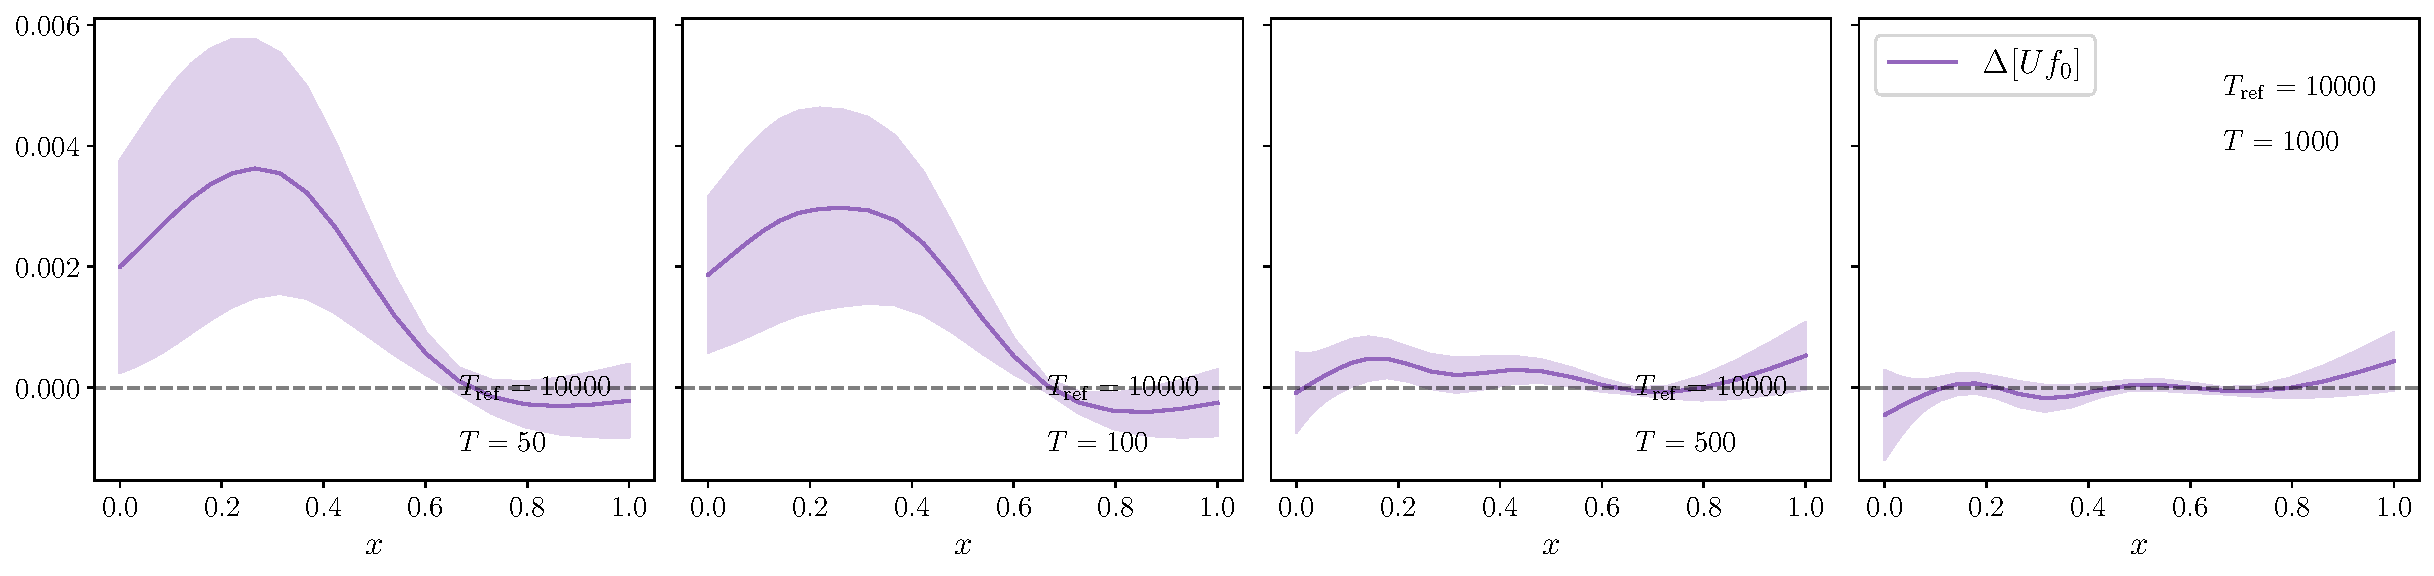
\includegraphics[width=0.95\textwidth]{section_4/delta_bootstrap_L2_U.pdf}
  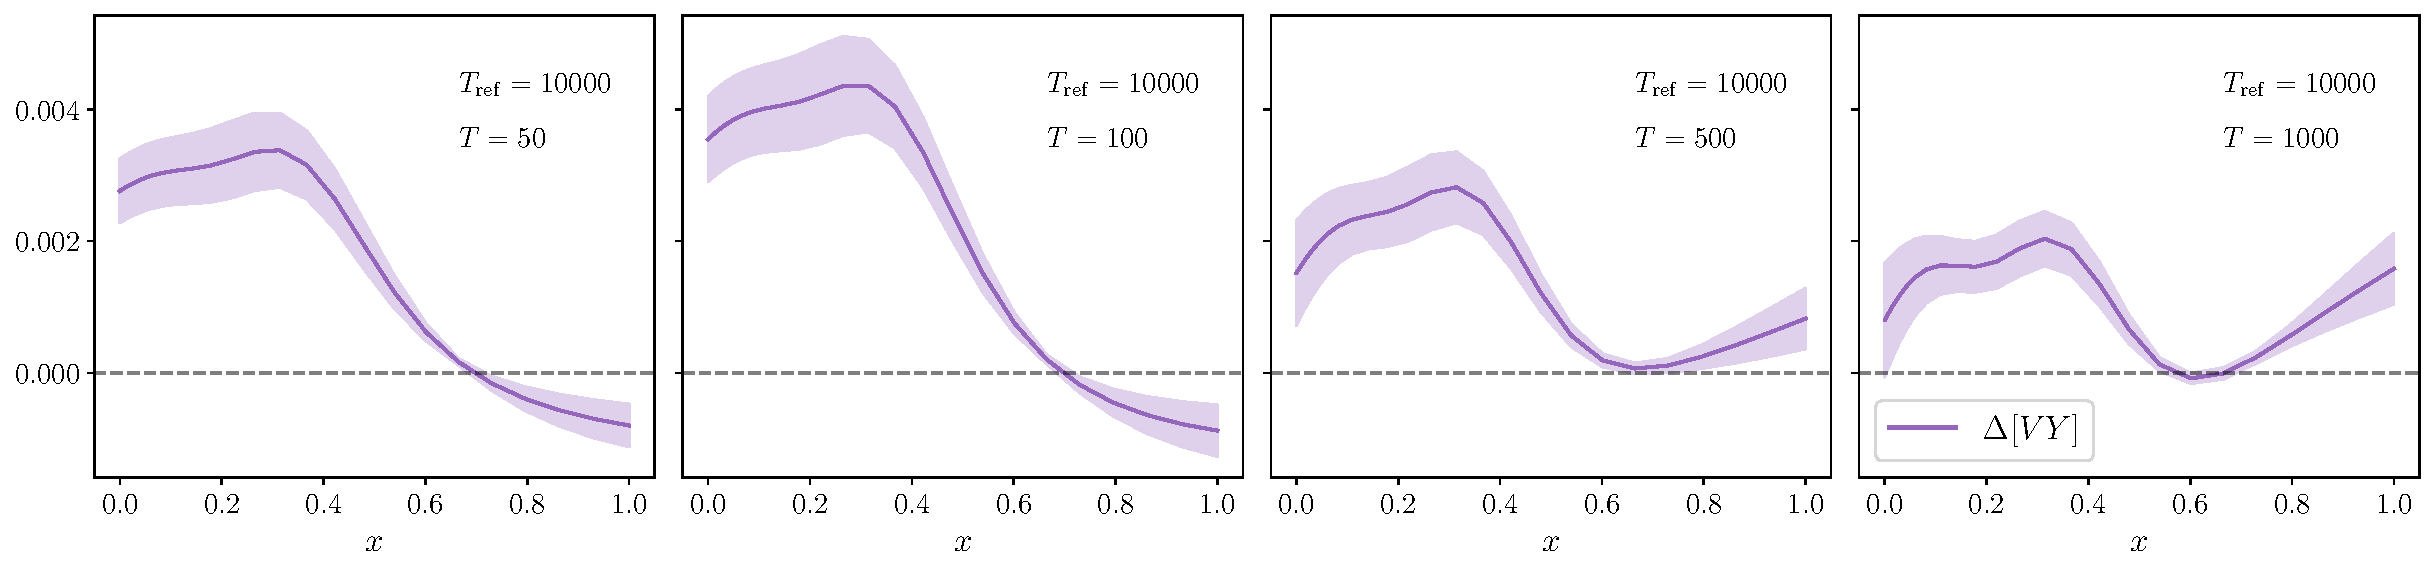
\includegraphics[width=0.95\textwidth]{section_4/delta_bootstrap_L2_V.pdf}
  \caption{Behaviour of $\Delta [U(t)f_0]$ and $\Delta [V(t)Y]$, as defined in
  Eqs.~\eqref{eq:DeltaExpValUtF0} and~\eqref{eq:DeltaExpValVtY}, as functions
  of the training
  time. The operators $U(T)$ and $V(T)$ are constructed by taking the 
  NTK at $T_{\rm ref} = 10000$, which is fixed across panels. The uncertainties are extracted
  from the bootstrap ensemble as discussed in the text.}
    \label{fig:xT3_exp_val}
\end{figure}
% ===================================

We can consider a simplifying limit of Eq.~\eqref{eq:MeanValAtT}, where the
initial condition $f_0$ and the data $Y$ are statistically independent
from the respective
evolution operators $U(t)$ and $V(t)$. Note that the first term on the right-hand
side of Eq.~\eqref{eq:MeanValAtT} can only be non-zero because of the
correlations between $U(t)$ and $f_0$. In the absence of such correlations, the
first term would be given by the product of the expectation values and therefore
would vanish if $f_0$ is an ensemble of networks at initialisation. Under these
assumptions, we have
\begin{align}
    \label{eq:MeanUt}
    \bar{U}(t)
        &= \mathbb{E}\left[U(t)\right]\, , \\
    \label{eq:MeanVt}
    \bar{V}(t)
        &= \mathbb{E}\left[V(t)\right]\, ,
\end{align}
and
\begin{equation}
    \label{eq:MeanValAtTNoCorr}
    \bar{f}_{t,\alpha} = \bar{U}(t)_{\alpha\alpha'} \bar{f}_{0,\alpha'}
        + \bar{V}(t)_{\alpha I} Y_I = \bar{V}(t)_{\alpha I} Y_I \, .
\end{equation}
The second term in Eq.~\eqref{eq:MeanValAtT}, or equivalently
Eq.~\eqref{eq:MeanValAtTNoCorr}, explicitly shows the contribution of each data
point to the central value of the trained fields at each value of $x_{\alpha}$.
It is worthwhile remarking that in this limit, the central value from the set of
trained networks is a linear combination of the data points, with coefficients
given by the evolution operator $V(t)_{\alpha I}$.

In the absence of general theorems, we verify this assumption empirically.
From the ensemble of replicas, we generate bootstrap samples and compute the
following two estimators,
\begin{align}
    \label{eq:DeltaExpValUtF0}
    \Delta[U(f)f_0] &= \mathbb{E}\left[U(t) f_{0}\right] 
      - \mathbb{E}\left[U(t) \right] \mathbb{E}\left[f_{0}\right]\, , \\
    \label{eq:DeltaExpValVtY}
    \Delta[V(f)Y] &= \mathbb{E}\left[U(t) Y\right] 
      - \mathbb{E}\left[V(t) \right] \mathbb{E}\left[Y\right]\, .
\end{align}
for different training times, using the same frozen NTK and L2 data. The results
are shown in Fig.~\ref{fig:xT3_exp_val} for the $U$ (upper panel) and $V$ (lower
panel) contributions. The error bands are computed using bootstrap error. By
inspecting the figures, we see two distinct patterns emerging. For the operator 
$U$, $\Delta[U f_0]$ is different from zero for small training times, and thus the
correlations between $U(t)$ and $f_0$ are non-negligible. However, as training
proceeds, the $\Delta[U f_0]$ becomes compatible with zero within the error bars, 
suggesting that the correlations are progressively suppressed.
The case of the $V$ operator is even more striking, as $\Delta[V Y]$ is clearly
non-negligible across all training times, although it also shows a decreasing trend as
training proceeds. This suggests that the correlations between $V(t)$ and $Y$
cannot be neglected. 

In conclusion, we note that Eq.~\eqref{eq:MeanValAtTNoCorr} resembles the structure
of a linear method, like \eg\ Backus-Gilbert or Gaussian Processes. We believe
that this observation, as well as the results shown in
Fig.~\ref{fig:xT3_exp_val}, deserve further investigations, which we leave for
future work.

\paragraph{Error decomposition}
% ===================================
\begin{figure}[t!]
  \centering
  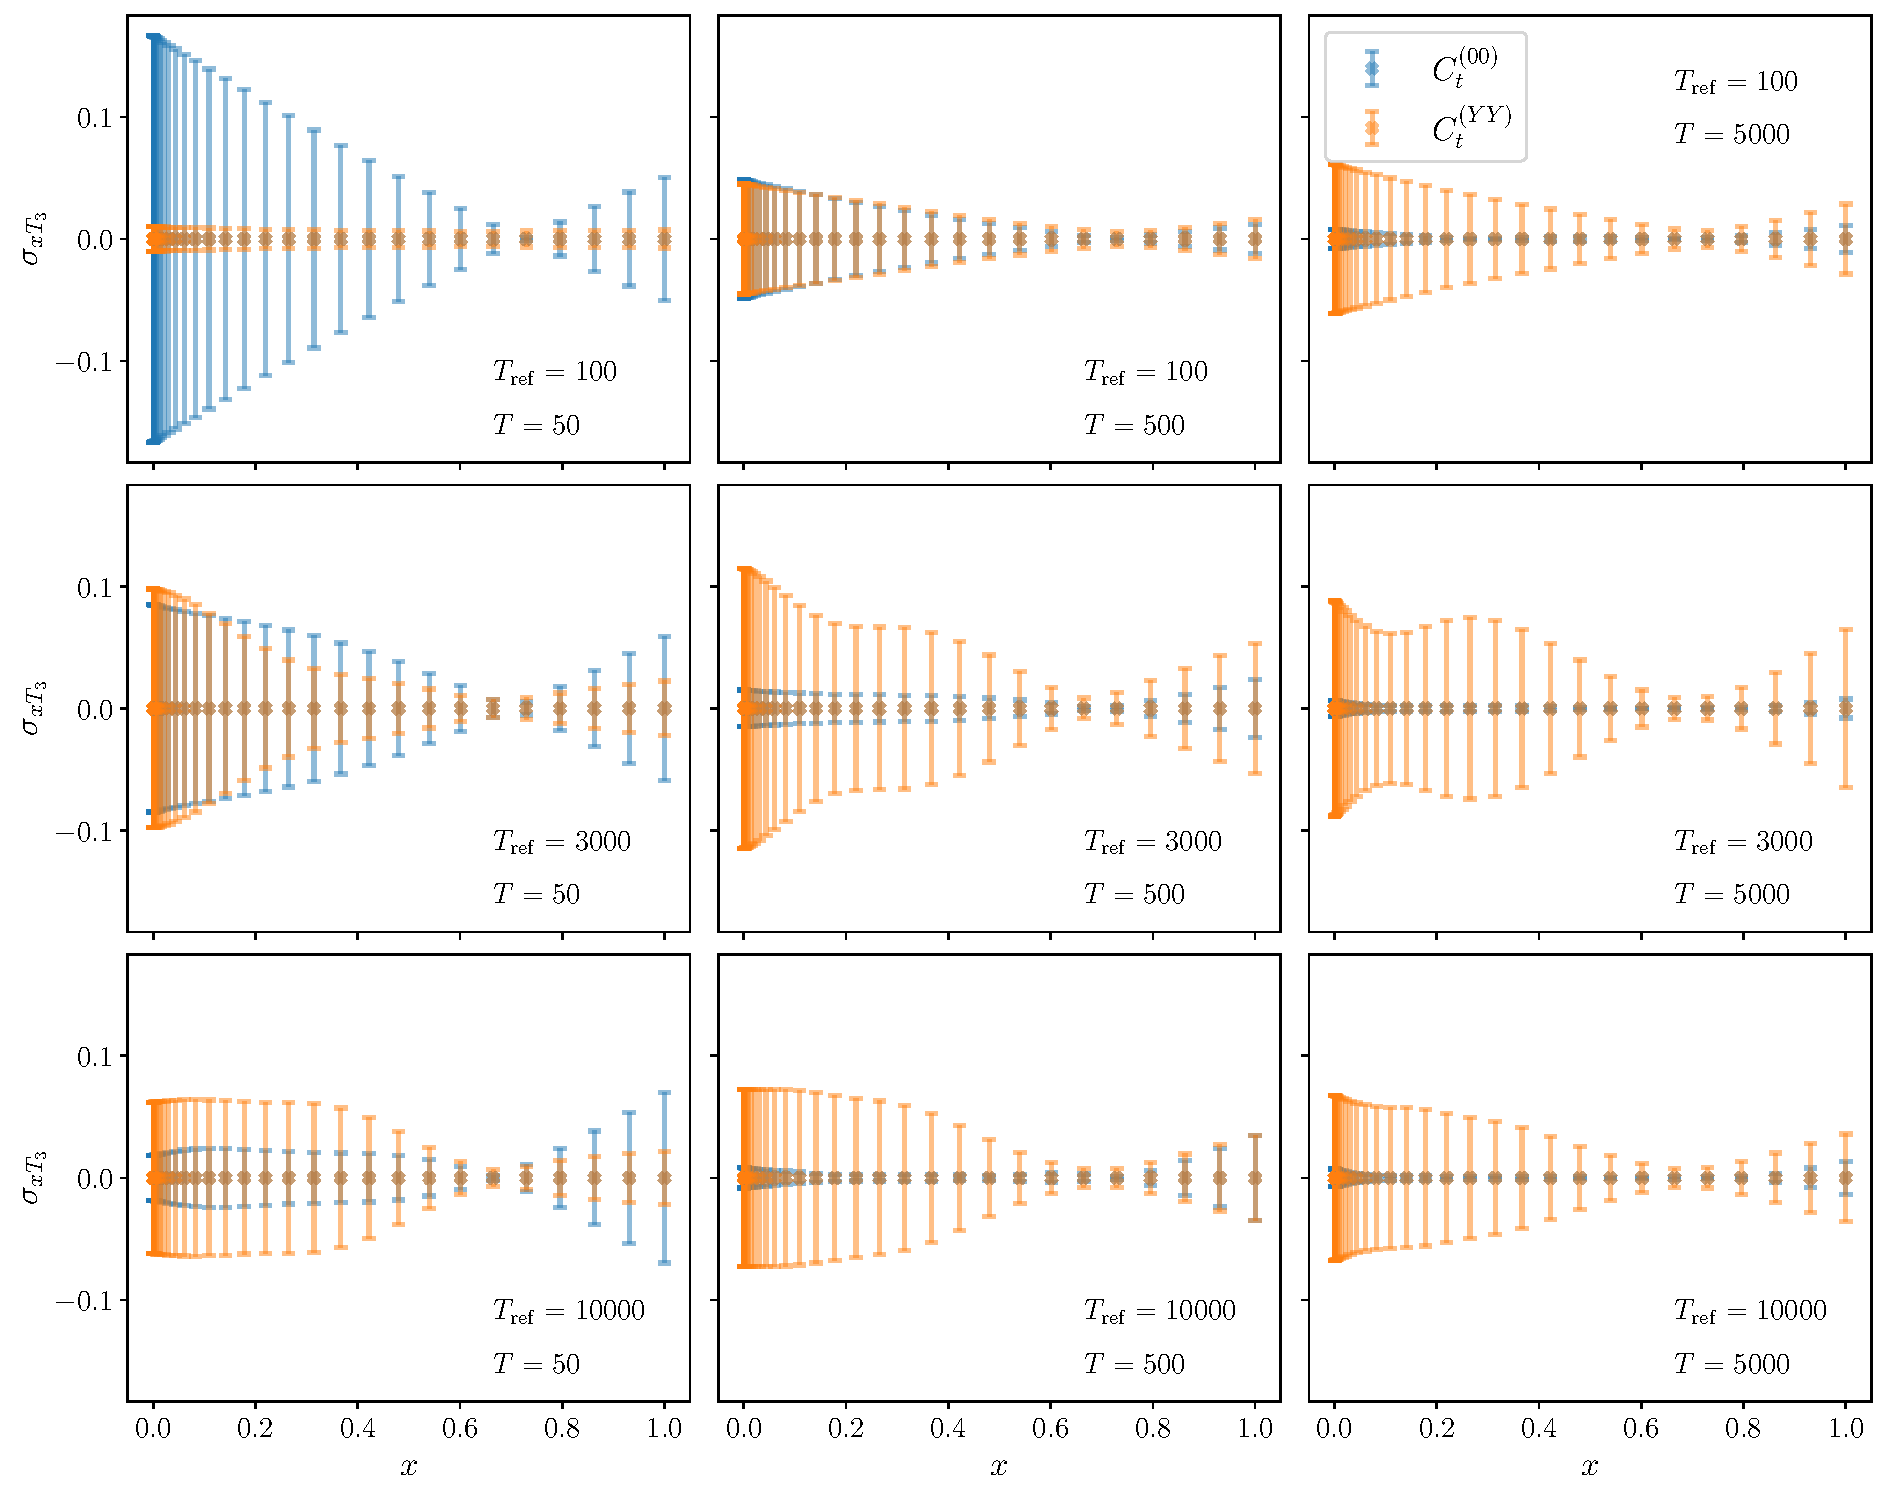
\includegraphics[width=0.9\textwidth]{section_4/error_buddget_L2.pdf}
  \caption{}
  \label{fig:ErrorBudgetL2}
\end{figure}
% ===================================
The analytical expression for the covariance matrix,
Eq.~\eqref{eq:SumOfCovariances}, allows us to monitor the relative size of the
three contributions as training proceeds. For a properly trained ensemble of 
networks, the covariance of the trained fields should be
dominated by the statistical error on the data. We show the diagonal entries of
the decomposition of the error budget in Fig.~\ref{fig:ErrorBudgetL2}, for
different frozen NTKs (rows) and different training epochs (columns), using L2
data as before. In general, we observe that towards the end of the training 
process the
contribution from the data $C_t^{(YY)}$ (orange band) becomes dominant with
respect to the contribution coming from the initial condition $C_t^{(00)}$ (blue
band). We also see that the suppression of the initial condition is more severe
and happens earlier when the frozen NTK is taken at later stages of training.
These findings ensure that the quoted error on the PDFs is actually dominated by
the statistical error on the data, and not by the fluctuations of the initial
fields. This is a crucial point, since it guarantees that the error bars computed
from the ensemble of
trained PDFs is not biased by the choice of prior that is made by selecting a
given architecture, activation function, and probability distribution for the
biases and weights at initialisation.

\subsubsection{Crosschecks using L0 data}
\label{sec:AnalyticalChecks}

The analytical solution enables rigorous validation of our implementation 
through crosschecks with L0 data, where we have complete control over 
the data generation process. In this case, the realization of the dataset is 
completely determined by the input PDFs
\begin{equation}
    \label{eq:DataL0NoIndices}
    Y = \FKtab \fin\, .
\end{equation}
Note that using L0 data only affects the second term in
Eq.~\ref{eq:AnalyticSol}.\footnote{To be more precise, since the analytical
solution requires the NTK to be frozen at a certain epoch $T_{\rm ref}$, the
NTK will depend on the data used in the training.} We can then rewrite
the combined term in Eq.~\eqref{eq:DataCorrectedInference} as follows
\begin{align}
  \label{eq:TrainingOnLevelZero}
  \check{U}^\perp(t) f_0 + V(t) Y 
    &= \mathcal{M}(t)\, \FKtabT C_{Y}^{-1} \FKtab\, 
      \left[\fin - f_{0}^\parallel\right]\, .
\end{align}
The subtraction taking place in the square brackets of
Eq.~\eqref{eq:TrainingOnLevelZero} suggests us that the effective function that
the neural network actually sees is not the input function $\fin$ used to
generate the data, but rather the difference between $\fin$ and the component of
the initial function $f_0$ that lies in the subspace spanned by the kernel of
the NTK, \ie\ $f_0^\parallel$. In other words, the parallel component
$f_0^\parallel$, which we remind does not evolve during the analytic training,
acts as a constant ``bias'' in the training process, shifting the effective
input function that the neural network sees. Of course the actual magnitude of
this irreducible noise depends both on how $f_0$ and the kernel of the NTK are
distributed over the ensemble. We will come to this point soon.

Note that the observation above remains true even in the limit of infinite
training. This can be shown using 
\begin{align}
    \label{eq:LevelZeroClosureInfiniteTraining}
    \lim_{t\to\infty} V(t) Y = \finperp + \mathcal{M}_{\infty} M \finpar\, ,
\end{align}
which shows that the $V$ component of the trained solution reproduces exactly the
component of the PDF that lies in  the subspace orthogonal to the kernel of
$\Theta$. We compare the asymptotic behaviour of $V(t) Y$ and $\finperp$ in
Fig.~\ref{fig:InfiniteTimeVterm}.

\begin{figure}[t]
  \centering
  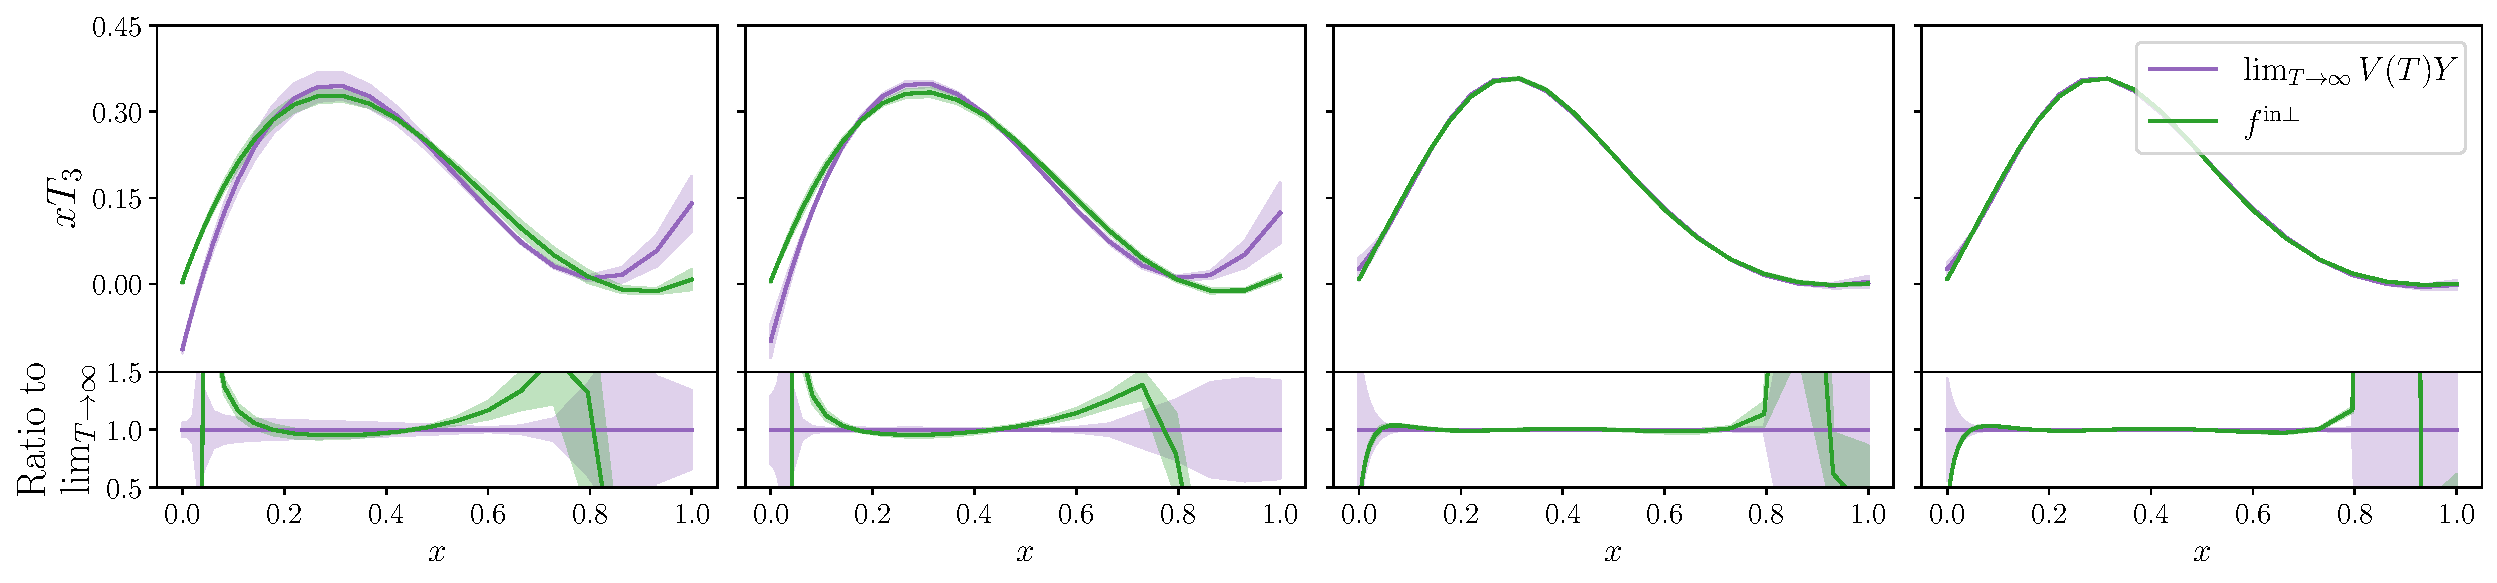
\includegraphics[width=\textwidth]{section_4/vy_inf_L0.pdf}  
  \caption{Test the $t\to\infty$ limit of the L0 training for different frozen
  NTK. The orange curve represents the projection of the input function $\fin$
  onto the subspace orthogonal to the kernel of the NTK at $T_{\rm ref}$, \ie\
  $\finperp$. The blue curve represents the contribution of the operator $V$,
  computed with the NTK at $T_{\rm ref}$, in the limit of infinite training
  time.}
  \label{fig:InfiniteTimeVterm}
\end{figure}

The second term in the square bracket on the right-hand side of
Eq.~\eqref{eq:TrainingOnLevelZero} is the contribution from the parallel
component at initialisation that does not evolve in the training process. Given
that $f_0$ is almost normally distributed around zero, that term does not
contribute to the central value of the fitted PDF, \ie\ to the average of the
trained solution over replicas. The time evolution of 
\begin{align}
  \label{eq:AverageLevelZeroUcheck}
  \mathbb{E}\left[\mathcal{M}(t)\, \FKtabT C_{Y}^{-1} \FKtab\, 
    f_{0}^\parallel\right]\, ,
\end{align}
is shown in Fig.~\ref{fig:AverageLevelZeroUcheck}.
\begin{figure}[h!]
  \centering
  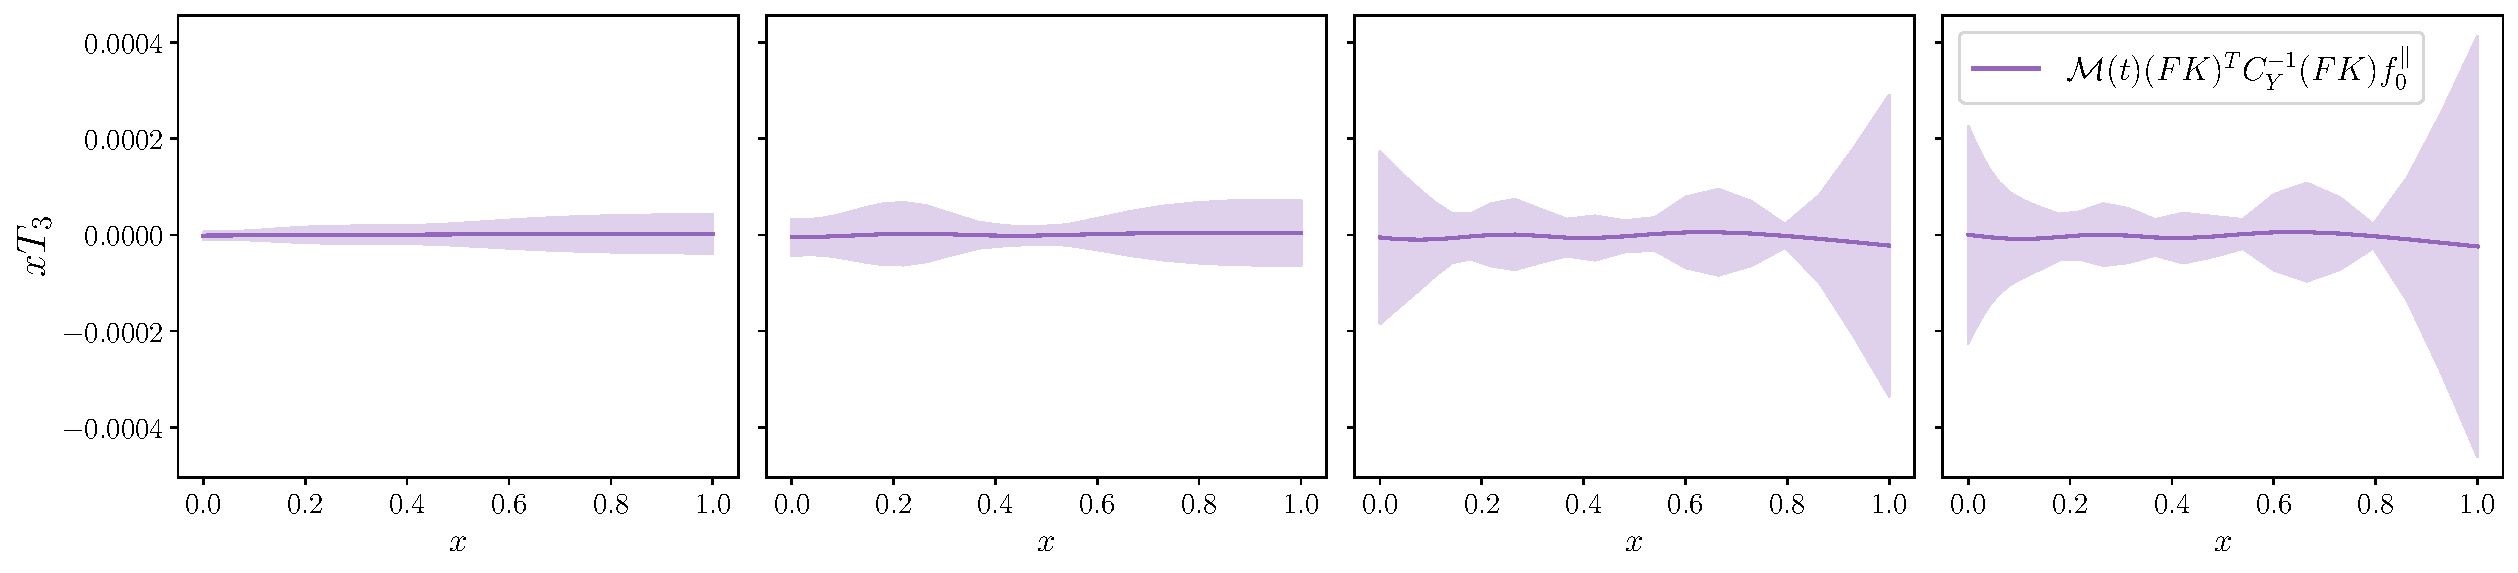
\includegraphics[width=0.95\textwidth]{section_4/Mcal_M_fpar_L2_linear.pdf} 
  \caption{Test of the average of the parallel contribution for different
  epochs. The reference epoch at which the frozen NTK is chosen is $T_{\rm ref}
  = 10000$. L2 data is used in the plot.}
  \label{fig:AverageLevelZeroUcheck}
\end{figure}

\subsubsection{Infinite Training Time}
In the limit of infinite training time, the evolution operators $U(t)$ and
$V(t)$ simplify and yield an elegant interpretation of the minimum of the cost
function. For large training times, we have
\begin{align}
    \label{eq:UhatInfty}
    \hat{U}^\perp_{\infty, \alpha\alpha'}
        &= \lim_{t\to\infty}\hat{U}^\perp(t)_{\alpha\alpha'} = 0\, \\
    \label{eq:MOperatorInfty}
    \mathcal{M}_{\infty, \alpha\alpha'} 
        &= \lim_{t\to\infty}\mathcal{M}(t)_{\alpha\alpha'} = \sum_{k,k'\in\perp} \sqrt{\lambda^{(k)}} z^{(k)}_\alpha 
        \left[\sideset{}{'}\sum_{i} w^{(i)}_{k} \frac{1}{h^{(i)}}\, 
        w^{(i)}_{k'}\right] z^{(k')}_{\alpha'} \sqrt{\lambda^{(k')}}\, ,
\end{align}
and explicit expressions for $\check{U}^\perp_{\infty}$ and $V_{\infty}$ are
obtained from $\mathcal{M}_{\infty}$. The term in the square bracket in
Eq.~\eqref{eq:MOperatorInfty} is the spectral decomposition of the pseudoinverse
of $H^\perp$ in $d_\perp$ orthogonal subspace. So, the operator
$\mathcal{M}_{\infty}$ acts as follow on a field $f_{\alpha}$:
\begin{enumerate}
    \item The term on the right of the square bracket computes the coordinate
    $f_k$ introduced in Eq.~\eqref{eq:OrthogonalComponents}. The $f_k$ are a set
    of coordinates for the component $f^\perp$ of the field that evolves during
    training, 
    \begin{align}
        \label{eq:RightOfTheBracket}
        f^\perp = \sum_{k\in\perp} \sqrt{\lambda^{(k)}} f_k\, z^{(k)}\,  .
    \end{align}
    \item The term in the square bracket applies the pseudoinverse to the
    coordinates $f_k$, 
    \begin{align}
        \label{eq:ApplyPseudoInv}
        f'_k = \left(H^\perp\right)^+_{kk'} f_{k'}\, .
    \end{align}
    \item The final term on the left of the square bracket reconstructs the full
    field corresponding to the modified $f'_{k}$,
    \begin{align}
        \label{eq:LeftOfTheBracket}
        f^{'\perp} = \sum_{k\in\perp} \sqrt{\lambda^{(k)}} f'_{k}\, z^{(k)}\, .
    \end{align}
    
\end{enumerate}

As discussed at the end of Sect.~\ref{sec:Lazy} it is convenient to combine the
contributions of $\check{U}^\perp_{\infty}$ and $V_{\infty}$,
\begin{align}
    \label{eq:DataCorrectedInferenceAtInfty}
    \check{U}^{\perp}_{\infty} f_{0} + V_{\infty} Y 
        = \mathcal{M}_{\infty}\; \FKtabT C_Y^{-1} \left[Y - \FKtab f_{0}^{\parallel}\right]\, .
\end{align}
The contribution to the observables from the parallel components of $f$ does not
change during training, therefore that contribution is subtracted from the data
and the orthogonal components of $f$ are adjusted to minimize the $\chi^2$ of
the corrected data. The minimum of the $\chi^2$ in the orthogonal subspace is
found applying $\mathcal{M}_{\infty}$, \ie\ by projecting in the orthogonal
subspace, applying the pseudoinverse and finally recompute the full field as
detailed above.


\FloatBarrier


\section{Conclusions}
\label{sec:Conclusions}
We conclude that...

\section*{Aknowledgements}
...

\newpage

% Appendices
\appendix
\appendix
\section{The BCDMS dataset for $T_3$}
\label{app:dataset}

In this analysis we employ a simplified framework where one single flavour in
the PDFs is required to compute the theory predictions as in
Eq.~\eqref{eq:TheoryPred}. In this respect, following
Ref.~\cite{Candido:2024hjt}, we focus on the determination of the non-singlet
triplet PDF combination, defined as
\begin{equation}
T_3 = u^+ - d^+,
\end{equation}
where $u^+ = u + \bar{u}$ and $d^+ = d + \bar{d}$. By combining measurements of
the structure function $F_2$ on proton and deuterium targets from the BCDMS
collaboration~\cite{Benvenuti:1989fm}, one can construct the observable $F_2^p -
F_2^d$ which, at next-to-next-to-leading order (NNLO) in QCD and under the
assumption of isoscalarity for the deuterium nucleus, provides a clean probe of
the nonsinglet triplet PDF combination $T_3$. The factorization formula reads
\begin{equation}
F_2^p - F_2^d = C_{T_3} \otimes T_3,
\end{equation}
where $C_{T_3}$ is the corresponding Wilson coefficient computed in perturbative
QCD, and $\otimes$ is a short-hand notation that denotes the convolution as in
Eq.~\eqref{eq:TheoryPred}. The construction of the FK-tables needed to compute
the predictions, as well as the application of kinematic cuts and the
construction of the covariance matrix, are identical to
Ref.~\cite{Candido:2024hjt}, to which the reader is referred for further
details. In order to study the training dynamics in a clean environment where the
noise is controlled, we generate synthetic data using the closure test framework
developed by the NNPDF collaboration~\cite{NNPDF:2021njg,DelDebbio:2021whr}
where pseudo-data are generated from a known underlying law. We use the central
value of the non-singlet triplet $xT_3$ from the NNPDF4.0~\cite{NNPDF:2021njg}
release as the input law $\fin$. Furthermore, we generate three levels of
synthetic data following the standard NNPDF convention for closure tests. These
levels differ by the way the noise is included, and are labelled as Level 0 (L0),
Level 1 (L1) and Level 2 (L2) data. We now summarise their definitions in turn.

\paragraph{Level 0}
The pseudo-data are generated without any experimental noise, \textit{i.e.} by simply using
the input function and the FK-tables as follows
\begin{equation}
Y_{L0} =  \FKtab \fin.
\end{equation}
In this ideal scenario, the analysis should reproduce the input $\fin$, though
some residual reconstruction error may remain in the kinematic region not
covered by the FK-tables. Level 0 assess the intrinsic bias of the methodology,
as any neural network replica will be trained on the same data points $Y_{L0}$.

\paragraph{Level 1}
In this case, the experimental noise is added on top of L0 data, by sampling from the
multivariate normal distribution with the full experimental covariance matrix
$C_Y$ provided by the BCDMS collaboration
\begin{equation}
Y_{L1} =  Y_{L0} + \eta, \quad \textrm{where} \quad \eta \sim \mathcal{N}(0, C_Y).
\end{equation}
This case is closer to actual experimental data, where the ``true'' value is
blurred by the presence of noise. Note however that we are not yet propagating
the experimental uncertainties into the uncertainties of the fitted PDF, as the added
noise is fixed over all replicas.

\paragraph{Level 2}
Finally, we generate L2 pseudo-data by adding a different noise realisation to each
replica, sampled from the same multivariate normal distribution
\begin{equation}
Y_{L2}^{(k)} =  Y_{L1} + \xi^{(k)}, \quad \textrm{where} \quad \xi^{(k)} \sim \mathcal{N}(0, C_Y).
\end{equation}
This represents the most realistic scenario where both model and data uncertainties
are present. In this case, each neural network replica will be trained on a
different set of data points $Y_{L2}^{(k)}$.
\section{Dependence on the Architecture of the NTK}
\label{sec:NTKArchDep}

It is interesting to consider what happens to the picture sketched so far as the
architecture of the neural networks is varied. In Fig.~\ref{fig:NTKTimeDiffArch}
we compare the time dependence of the Frobenius norm of the NTK and the
variation of the first three eigenvalues for two different architectures. The
smaller network is the $[28,20]$ used in the standard NNPDF analyses and in this
work, while the large one is a $[100,100]$ network, which is closer to the
infinite-width limit. For illustration purposes we focus in this plot on L1 data
and only three eigenvalues rather than the five we examined above. The
quantitative features are exactly the same for L0 and L2 data, and adding the
fourth and fifth eigenvalues does not add unexpected behaviours compared to what
we observe in Fig.~\ref{fig:NTKTime}. It is interesting to remark that the onset
of lazy training is slower for the larger network. This is to be expected if we
interpret the early stages of training as a phase where the network identifies
the learnable features in the space of functions that it can parametrize. For a
larger network, the space of parametrized functions is larger and the
identification of the physical features takes a larger number of epochs. 
% ===================================
\begin{figure}[t]
  \centering
  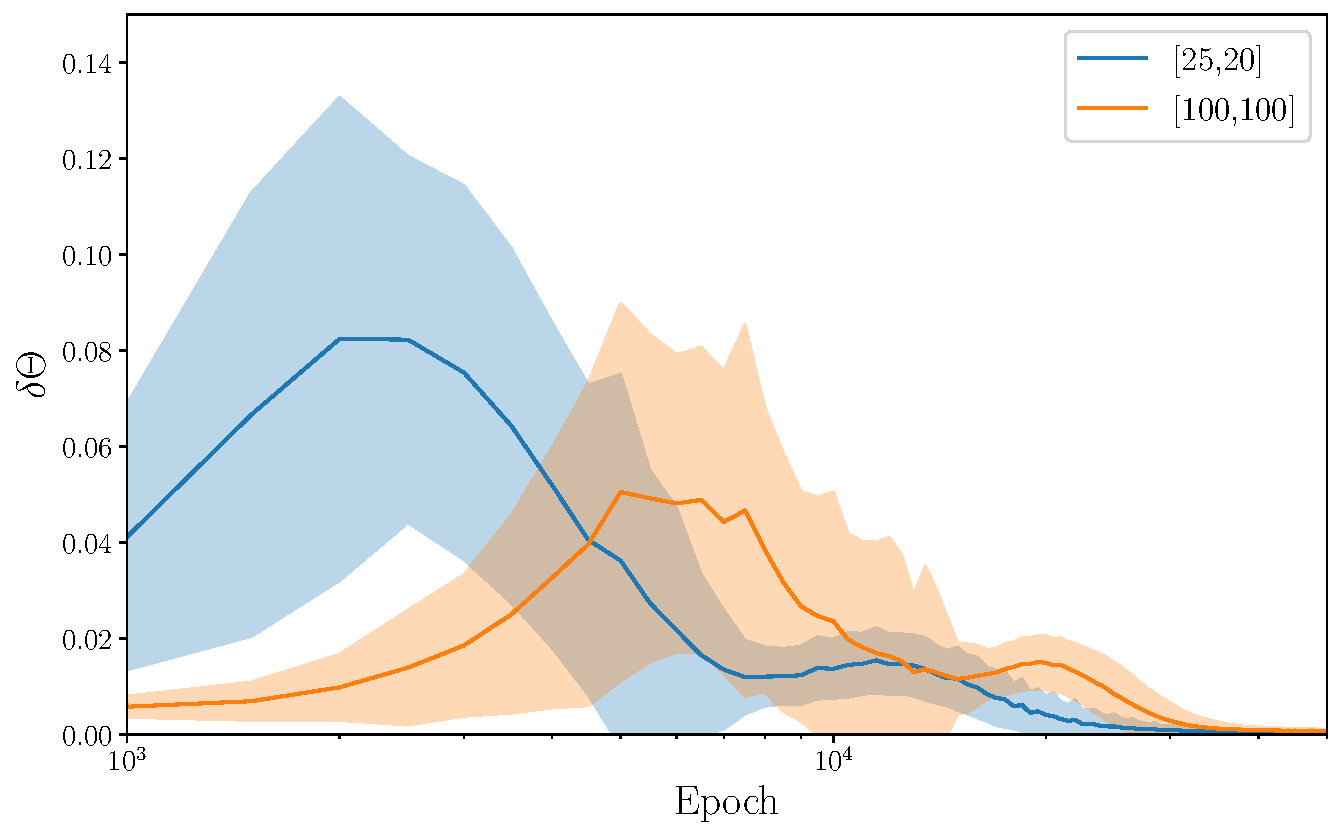
\includegraphics[width=0.45\textwidth]{appendix_arch/delta_ntk_arch.pdf}
  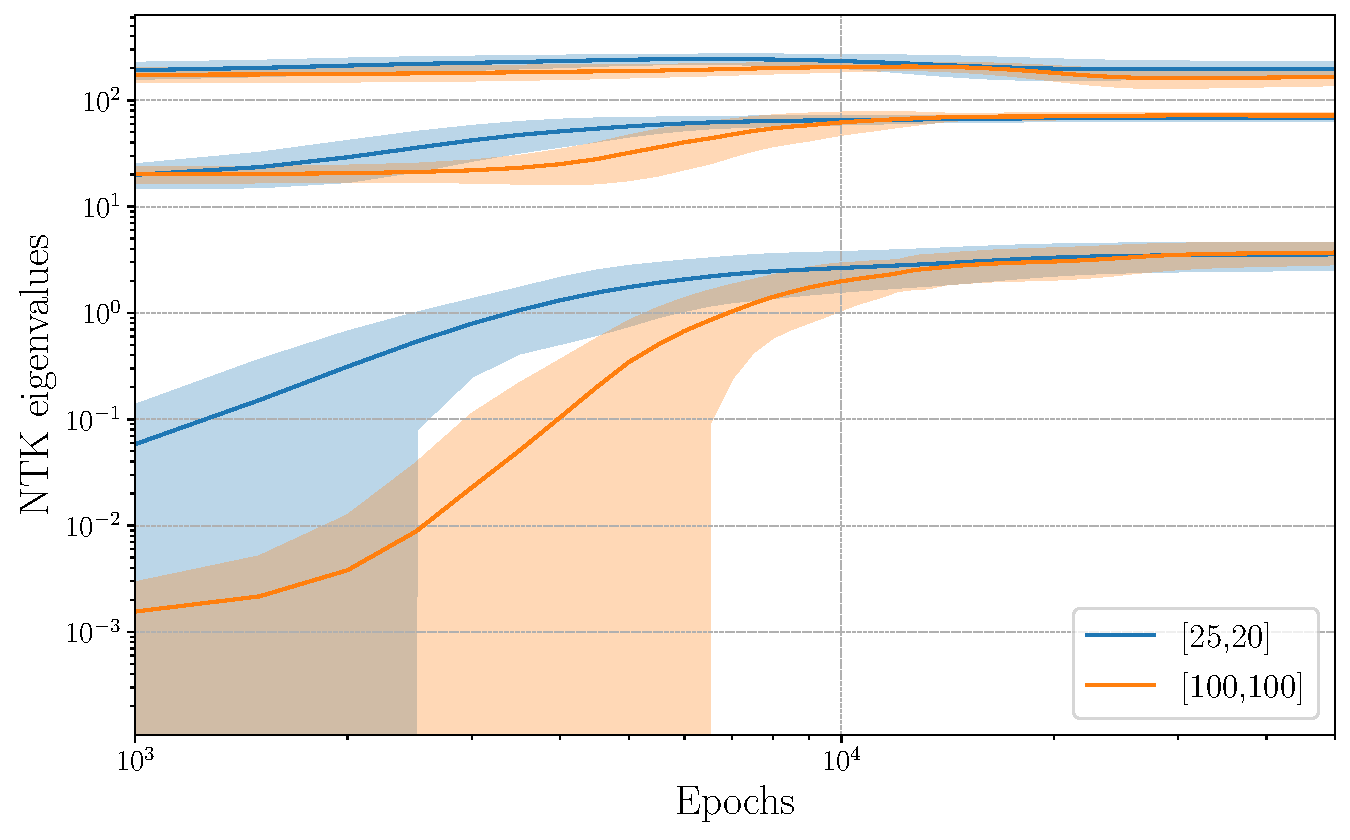
\includegraphics[width=0.45\textwidth]{appendix_arch/ntk_eigvals_single_plot_arch.pdf}
  \caption{Comparison of the variation of the NTK during training (left) and the
  first three eigenvalues (right) for two different architectures with sizes
  $[28,20]$ and $[100,100]$ respectively. In both cases, L0 data is used. In the
  left plot, error bands represent the standard deviation over the ensemble of
  replicas. In the right plot, solid lines represent the median over the
  ensemble of networks, while solid bands correspond to 68\% confidence level.}
  \label{fig:NTKTimeDiffArch}
\end{figure}
% ===================================

\FloatBarrier

% Bibliography
\bibliographystyle{unsrt}
\bibliography{ntk.bib}

\end{document}